% LuaLaTeX-Dokument! Codierung: Unicode, UTF-8. Schriftart: Linux Libertine Normal, Schriftgröße 10. Druck auf DIN A5. Hardcover only! Fnbsrd ist kein Taschenbuch.
%
% Lizenz: Siehe Ende des Buches

\begin{filecontents*}{fnbsrd-01.xmpdata}
    \Title{Fnbsrd}
    \Author{Tobias Frei, fnbsrd.de}
    \Copyright{Tobias Frei, fnbsrd.de}
    \Org{fnbsrd.de}
    \PublicationType{book}
    \Keywords{German\sep novel\sep fantasy\sep freely licensed\sep open source}
    \Subject{Einführung in eine Fantasy-Welt mit Elfen, Drachen und Menschen, drei verfeindeten Königreichen und voller Magie. Open Source, geschrieben in LaTeX (LuaTeX).}
\end{filecontents*}
% Nach Änderungen am xmpdata-Abschnitt muss die ".xmpdata"-Datei manuell gelöscht werden.

\documentclass[paper=a5,pagesize=auto,fontsize=10pt,div=14,BCOR=15mm]{scrbook}
% Dabei gilt:
%     A5 ist die Papiergröße,
%     pagesize=auto
%     10pt ist die Schriftgröße,
%     div=14 beeinflusst unter anderem die Randgröße. Einen perfekten Wert gibt es nicht.
%     BCOR=15mm fügt 15 Millimeter Bindekorrektur an den Innenrändern hinzu.

%\usepackage{colorprofiles}
% "sRGB_IEC61966-2-1_black_scaled.icc"-Farbprofil für das "pdfx"-Paket
% Wird nicht benötigt, da das frei lizenzierte Farbprofil einfach als ".icc"-Datei mitgeliefert wird.
% Falls die Datei fehlen sollte, genügt es nicht, diese Zeile auszukommentieren.
% Die im Paket "colorprofiles" enthaltene Datei müsste zudem umbenannt werden,
% sonst wird sie nicht gefunden. ("sRGB_IEC61966-2-1_black_scaled.icc")
% Noch ein Fallstrick:
% Manche Dateisysteme unterscheiden zwischen Groß- und Kleinschreibung.

\usepackage[a-1b]{pdfx}
% "PDF-A/1-b"-Standard einhalten; Konformität in den PDF-Metadaten ankündigen und einfordern.

\usepackage{hyperref}
% Verlinkung im Inhaltsverzeichnis.
% Enthalten in "pdfx", daher ohne Zusatzoptionen wie "hidelinks", sonst gibt es eine Fehlermeldung.

\hypersetup{
    colorlinks=false,
    pdfborder={0 0 0},
}
% pdfx-kompatible Alternative zu "hidelinks":
% Links nicht in bunter Schrift darstellen, keine roten Kästen um Links darstellen.

\usepackage{polyglossia}
% Das hieß früher "babel". Polyglossia ist der Nachfolger.

\setdefaultlanguage[spelling=new, babelshorthands=false]{german}
% Neue deutsche Rechtschreibung,

\usepackage{fontspec}

\setromanfont{Linux Libertine}
\setsansfont{Linux Biolinum}
\setmonofont{Linux Libertine Mono}
% ausschließlich frei lizenzierte Schriften verwenden.

%% Fallback:
%\setromanfont[Path=~/.fonts/,BoldFont=linlibertine_rbah.ttf,ItalicFont=linlibertine_riah.ttf,UprightFont=linlibertine_rah.ttf]{Linux Libertine}
%\setsansfont[Path=~/.fonts/,BoldFont=linbiolinum_rbah.ttf,ItalicFont=linbiolinum_riah.ttf,UprightFont=linbiolinum_rah.ttf]{Linux Biolinum}
%\setmonofont[Path=~/.fonts/,UprightFont=linlibertine_mah.ttf]{Linux Libertine Mono}
%% ausschließlich frei lizenzierte Schriften verwenden.

\usepackage{microtype}
% Zeilenränder glätten durch minimal veränderte Buchstabenabstände (Blocksatz).
% Dabei wird nicht mathematisch exakt eine Randlinie gezogen,
% sondern der optische Eindruck beachtet.
% "Löcher" durch Punkte und Bindestriche am rechten Rand werden vermieden,
% indem diese Zeichen ein kleines Stück über den Rand hinaus geschoben werden.

\usepackage{graphicx}
% Einbinden von Bildern. PDF ist dabei ein gültiges Bildformat.

\usepackage{pdfpages}
% Einbinden von PDF-Seiten als 1:1-Kopie, wenn Verkleinerung nicht gewünscht ist.

\setlength{\emergencystretch}{2em}
% Der Blocksatz darf auch größere Leerzeichen (bis zu 2 em breit) enthalten.

\typearea[15mm]{14}
% Sehr wichtig: Der Seitenrand muss an dieser Stelle, nachdem alle Schriftarten geladen wurden, neu berechnet werden.
% 15mm sind die Bindekorrektur, 14 ist der DIV-Wert.
% Mehr DIV = kleinere Ränder.

\hyphenation{da-rauf-hin} % statt "da-r-auf-hin"
\hyphenation{Dis-tanz} % statt "Di-s-tanz"
\hyphenation{dis-tanz-ab-hän-gi-ge} % statt "di-s-tanz-ab-hän-gi-ge"
\hyphenation{grauen-haft} % statt "grau-en-haft"
\hyphenation{He-li-kop-ter} % statt "He-li-ko-p-ter"
\hyphenation{über-ei-nan-der} % statt "über-ei-n-an-der"
\hyphenation{Wand-en-de} % statt "Wan-d-en-de"
\hyphenation{wa-rum} % statt "wa-r-um"
% Besondere Silbentrennungen: Unschöne, nicht empfohlene, aber erlaubte Trennungen ausschließen.

% == Semantik-Leitfaden ==
% \emph für Betonung verwenden ("emphasis", HTML-"em"-Tag),
% \textbf für wichtigen Text verwenden ("bring attention to", HTML-"b"-Tag),
% \textit für Lautsprecherstimmen und zitierten Text verwenden ("alternative voice", HTML-"i"-Tag),
% falls vorhanden, stattdessen IA-spezifische Befehle verwenden:

\newcommand{\ialoudspeaker}{\textit} % Lautsprecherstimmen. \ialoudspeaker{»G4 Richtung Hongkong, 26 Kilometer Stau. G1 …«}
\newcommand{\iaquote}{\textit} % Zitate. \iaquote{»Zuerst die Lok aufbügeln …«}
\newcommand{\iashout}{\emph} % Laute Rufe. »Drehen Sie \iashout{sofort} um und landen Sie auf dem Flughafen!«
\newcommand{\iathought}{\emph} % Gedanken. \iathought{Halsabschneider}, dachte yury. »Das ist ein guter Preis.«
% Eigene Befehle, damit nachträglich einfach die Formatierung bestimmter Textarten geändert werden kann.

\begin{document}

\pagestyle{plain}
% Keine Kapitelüberschrift in der Kopfzeile; nur Seitenzahlen in der Fußzeile.

\extratitle{\textbf{Fnbsrd}\\Originale deutschsprachige Fassung~– nicht übersetzt.\\© Tobias Frei, fnbsrd.de

\bigskip

\noindent Dies ist eine offizielle Ausgabe des ersten Fnbsrd-Romans, herausgegeben von Tobias Frei. Veränderte Versionen und unautorisierte Nachdrucke müssen deutlich als solche erkennbar sein. Auch das Impressum muss angepasst werden, wenn das Dokument verändert wird.

\bigskip

\noindent Der gesamte Buchinhalt wurde unter einer freien Lizenz veröffentlicht. Mehr Informationen befinden sich auf den letzten Seiten des Buches.

\bigskip

\noindent Gedruckt mit Wassermagie in der Lindenbibliothek von Last Hope.}

\title{Fnbsrd}

\subtitle{Der Hilferuf des Drachen}

\author{Tobias Frei\\ fnbsrd.de}

\date{} % Ein "leeres Datum" entfernt die Datumsangabe auf der Titelseite.

\dedication{für Oliver Knörzer}

\lowertitleback{\noindent Texte: © Tobias Frei, fnbsrd.de

\bigskip

\noindent Der gesamte Buchinhalt ist frei lizenziert; die Lizenz ist am Ende des Buches abgedruckt. Solange es die offizielle Website gibt, kann das gesamte Material inklusive LaTeX-Quelltext dort heruntergeladen werden. Ich freue mich, wenn Du die Möglichkeiten der Lizenz nutzt und Fnbsrds Geschichte in der Welt verbreitest.

\bigskip

\noindent Dieses Dokument enthält Internetlinks, die zum Zeitpunkt der Veröffentlichung von mir geprüft wurden. Den Inhalt der verlinkten Seiten mache ich mir allerdings nicht zu eigen; ich habe keine Kontrolle über spätere Veränderungen des verlinkten Inhalts. Sollte entgegen meinen Erwartungen eines Tages ein Link defekt oder sogar schädlich bzw. unangemessen geworden sein, bitte ich um eine Benachrichtigung per Post. Ich werde solche Links dann schnellstmöglich aus weiteren Ausgaben entfernen. Da ich keine Haftung für die Sicherheit der Links übernehmen kann, erfolgt der Aufruf der verlinkten Seiten auf eigene Gefahr.

\noindent \textbf{Die Handlung des Romans ist fiktiv, absurd und nicht zur Nachahmung geeignet.} Etwaige Ähnlichkeiten mit tatsächlichen Begebenheiten oder lebenden oder verstorbenen Personen wären rein zufällig. Der gesamte Inhalt des Buches wurde frei erfunden.

\bigskip

\noindent Erste Auflage, erschienen 2023-07-01

\noindent Verlag \& Herausgeber:\\
\noindent Tobias Frei\\
\noindent Böhler Weg 19\\
\noindent 42285 Wuppertal\\
\noindent impressum@tfrei.de}

\maketitle

\tableofcontents

\newpage

\part{Exodus}

\chapter{No Sympathy}

Ein Junge im schwarzen T-Shirt, etwa drei Schneiderellen groß, mit schwarzen Haaren und pechschwarzen Iriden unter einer Sonnenbrille rückte sich die schwarzen Socken unter der schwarzen Jeans zurecht, damit diese besser in die schwarzen Klettschuhe passten. Dann erhob er sich und blickte sich um. Seine Kleidung schluckte das einfallende Licht und wäre selbst im Dunkeln durch starken Kontrast aufgefallen. So anziehend wie das alles für das Licht wirkte, so abstoßend war es für die Mitmenschen im Restaurant. Fnbsrd hatte sich in den vergangenen dreizehn Jahren bei jeder Gelegenheit äußerst unbeliebt gemacht; nur die Zivilisiertheit der fortschrittlichen Stadt hatte einen Lynchmord verhindert.

Der ältere Herr am Tisch zu seiner Rechten sah einigermaßen sympathisch aus.

»Verzeihen Sie. Stört es Sie, falls ich mich zu Ihnen setze?«

»Wenn jemand fragt, ob sein Gegenüber eine ehrliche oder eine freundliche Antwort erwartet, dann steckt im Wort ›oder‹ bereits eine unfreundliche Antwort.«

Das klang sehr allgemein gehalten. »M … hm?«

»Und deshalb kann ich das nicht fragen.«

Es handelte sich um die wohl freundlichste Ablehnung, die er je hören musste. Er nickte betrübt und machte Anstalten, zum nächsten Tisch zu gehen. »Ich danke Ihnen für Ihre diplomatische Ausdrucksweise.«

»Gerne. Und jetzt zieh Leine.«

\begin{center}
∞∞∞
\end{center}

»Die Leute mögen dich nicht, Fnbsrd«, rief Göländör ihm während des Essens noch einmal in Erinnerung. Es bestand keine Aussicht darauf, das Thema zu wechseln.

»Das weiß ich doch«, seufzte Fnbsrd gelangweilt. »Man kommt sich fast vor, als fände diese Unterhaltung in einem Dorf statt, in dem jeder jeden kennt und noch mit Holz geheizt wird.«

Ein interessanter Punkt. »Vielleicht solltest du dorthin gehen«, schlug der Elf ernsthaft vor. »Vielleicht hat man dort mehr Verständnis.«

»Verständnis wofür?«, fragte Fnbsrd.

»Für jemanden, der mit dem Feuer spielt und seine Umgebung in Flammen setzt, aber keine Elementarzauber zur Beherrschung der Katastrophe kennt.«

»Ich bin Künstler! Ich habe keine Muße und keinen Bedarf an Elementarzaubern. Feuer, Wasser, Wind … Das sollen andere erledigen. Mein Metier ist die Schaffung, Veränderung und Reparatur von Leben, von Welten, von Weltsteinen.«

»Du bist ein Nichtsnutz. Zum Heiler hat es gerade so gereicht; mit brandgefährlichen Steinen ist kein Geld zu verdienen. Jeder, der ein Feuer entzünden möchte, kann das mit Grundschulzaubern in seinem Ofen tun. Du kannst nicht einmal das wirklich gut.«

»Die Schule verdirbt die Kinder«, echauffierte sich Fnbsrd. »Sie bereitet sie darauf vor, namenlos in ein System integriert, von diesem verschluckt und bedeutungslos zugrundegearbeitet zu werden. Am Ende steht ein Häufchen Asche, das als Dünger verwendet wird. Mich ekelt diese Gesellschaft an!«

»Oho, das beruht auf Gegenseitigkeit. Iss auf, ich habe nicht den ganzen Tag Zeit, dich zu beaufsichtigen.«

Fnbsrd explodierte innerlich. Nach außen zischte es. »Würde es dir etwas ausmachen, wenn ich mich dabei verschlucke?«

»Willst du eine ehrliche oder eine freundliche Antwort?«

\begin{center}
∞∞∞
\end{center}

Fnbsrd spielte seit Längerem mit dem Gedanken, Blautal den Rücken zu kehren und den Berg zu verlassen. Um die »Nabe«, die Bergspitze, herum gab es noch zwei weitere Dörfer: Grüntal, das Dorf eines blutrünstigen Elfenkönigs, und Rottal, das Dorf eines weisen Drachenherrschers. Blautal wurde von einem scheuen Menschen regiert, der in seiner Angst vor Fremden unzählbare Seelen auf dem Gewissen hatte. Sprechenderweise hieß der Elf »Thürstön«, der Drache »lyssenko« und der Mensch »Xenophob«. Die drei Könige der Talstädte kamen dem, was manche sich unter Göttern vorstellen, sehr nah; ihr Kontakt zur Außenwelt war seit Langem durch Magie und fehlenden physischen Kontakt geprägt. Ihre Unsterblichkeit bezogen sie durch Nekromantie aus dem Leben ihrer Untertanen. Ein paar Sommer weniger Lebenszeit für jeden Einzelnen fielen kaum ins Gewicht; den Königen bescherte es das Überdauern der Jahrtausende. Früher in Kriegen, heute in Angst. Kalt und abstoßend war das alles.

Um den Berg herum führten niedere, schlecht entwickelte Dörfer als Stellvertreter den Krieg der Herren untereinander. Wer in der Gunst des Grüntals kämpfte, erhielt vom Elfenkönig und seinen Untertanen Waffen zur Eroberung der unendlich großen Welt. Wer im Dienst des Drachen ein Dorf regierte, konnte mit strategischer Unterstützung rechnen, die ihm einen Vorteil gegenüber den wenigen gunstlosen Dörfern verschaffte, die in ihrer »Neutralität« stets am Abgrund standen. Der menschliche König Xenophob war ein Defensivkünstler, ein Mauernbauer, ein Burgarchitekt. Große Stadtmauern, die so nie von Hand einzelner Lebewesen erschaffen werden konnten, umgaben die von ihm unterstützten Kleinstädte.

Man konnte bei dieser Aufteilung als Fremder leicht auf den Gedanken kommen, in Blautal lebten hauptsächlich Menschen, im Grüntal hauptsächlich Elfen und im Rottal fast nur Drachen. Dem war nicht so. Und wer bei Magie und Drachen glaubte, diese seien im Umgang mit Feuer begabter als Elfen, der irrte ebenfalls gewaltig. Jedes Kind konnte zaubern, jeder Jugendliche war auf irgendeine Magieform spezialisiert, jeder Erwachsene war ein Erzmagier seiner Schule. Talent und Fleiß beim Üben der Zauber, die Wahl der Sprüche und der Spezialisierung waren niemandem durch seine Abstammung in die Wiege gelegt. Es gab talentiert wasserzaubernde Drachen ebenso wie Windmagier unter den Menschen. Trolle, Zwerge, viele mystische Wesen bevölkerten die magiegetränkte Welt, und keines von ihnen war intrinsisch zu einer Form der Magie gezwungen.

Fnbsrd hatte die Erschaffung von Weltsteinen für sich entdeckt. Schwarz wie seine Kleidung, aber in unsichtbar tiefem Rot glühend wie das Innere von Vulkanen, nur kompakter und gebändigter in den Händen erfahrener Künstler. Eine brotlose und gefährliche Kunst, denn Holz und die Steine vertrugen sich nicht. Mit modernen Portalen konnte man in diesen Steinen versinken, während draußen fast keine Zeit verging. Ein nahezu beliebig langer Ausflug in eine Gedankenwelt mit wirklich beliebig erschaffbaren Regeln und Charakteren. Der ideale Schlüssel zu unendlicher Weisheit, wenn man diese Steine zu nutzen wusste. Fnbsrd war gebildeter als die meisten Lehrer, überheblicher als sein König und ärmer als manche Bettler. Ein paar Heilzauber lagen in seinem Repertoire, vernachlässigt zugunsten der Kunst. Überlebensfähig war er durch das Mitleid seiner Mitmenschen, doch das hielt sich in Grenzen, wenn man zum wiederholten Male ganze Landstriche dem Feuer zum Opfer fallen ließ, nur weil man gedankenverloren einen Stein falsch abgelegt hatte.

Und so kam es, wie es kommen musste: Fnbsrd kehrte Blautal den Rücken und trat den Weg in die Tiefe am Fuß des Berges an. Was als »Talstadt« bekannt war, lag tausende Häuser hoch über dem Pöbel. Eine abgehobene Gesellschaft, die in ihrem Fortschritt versank und jede Sympathie verspielte.

»Auf Nimmerwiedersehen« war der Abschiedsgruß, zu dem sich wenigstens ein Elf herabließ. Es war Göländör, derjenige, der Fnbsrd gegenüber am wenigsten negativ eingestellt war. Sozusagen ein bester Freund. Alle anderen schickten stumm ein paar Flüche hinterher oder dankten dem König dafür, dass er sie von der Last erlöst hatte.

»Auf Nimmerwiedersehen. Ich werde euch nicht vermissen.«

Göländör musste das letzte Wort haben. »Wir dich auch ganz bestimmt nicht.«

\begin{center}
∞∞∞
\end{center}

Die Dorfmauern von Last Hope waren eine Eigenkonstruktion der darin lebenden Bewohner. Lehm, billige Ziegel, unregelmäßige Zinnen, aber immerhin bis zu zehn Meter hoch über den Boden ragend. Einen Burggraben gab es nicht; das Gebilde als »Burg« zu bezeichnen, war eine Beleidigung gegenüber den von Xenophob magisch unterstützten Architekturen in anderen Dörfern. Doch von Xenophob und Konsorten wollte hier niemand etwas wissen; Könige waren unwillkommenes Gesindel vom Berg.

\iathought{Beste Voraussetzungen für einen Besuch} sah Fnbsrd darin. Er klopfte von außen an das riesige hölzerne Doppeltor und ersuchte um Einlass.

»Wer sind Sie und was wollen Sie?«, schallte es ihm von oben entgegen.

Fnbsrd reckte seinen Kopf in die Höhe und rief zurück: »Ich bin die Dunkelheit und suche nach Licht.«

Das war ungewöhnlich genug, um eine Rückfrage bei einem Dienstälteren hervorzurufen. Mangels Telefon und Privatsphärebedürfnis schallte diese einfach über den Platz. Aus der Ferne hörte man eine eher murrende Antwort, dann trampelten Schritte näher. Ein roter Drache, etwa zweieinhalb Meter hoch und dennoch weit vom Torbogen entfernt, drückte mit seinen Klauen das Holz beiseite. Fnbsrd ahnte, dass Magie hinter der vorgeblichen Kraftdemonstration steckte, und zeigte sich entsprechend unbeeindruckt. »Moin.«

»Wer sind Sie?«, fragte der Drache mit tiefer, dröhnender Stimme. Aus seinen Nüstern züngelte das innere Feuer.

»Mein Name ist Fnbsrd.« Er sprach jeden Buchstaben einzeln aus, weil die Konsonanten sich absichtlich nur buchstabieren oder durch unanständige Vokale ergänzen ließen. Die Namenswahl war eine der vielen Gemeinheiten, mit denen man im Blautal sogar von seinen Erzeugern gestraft wurde.

Der Drache schnaubte vorsichtig. »Ein ungewöhnlicher Name. Und keine Antwort auf meine Frage.«

Fnbsrd blinzelte.

»Woher kommen Sie?«

»Blautal.«

Feuer!

»Brauchen Sie ein Taschentuch?«

Fnbsrd stand in einer Flammenwolke; um ihn herum verbrannte die spärliche Vegetation zu schwarzer Asche. Der Drache blinzelte; das Blatt hatte sich gewendet.

»Hören Sie, ich suche Zuflucht vor den Idioten meiner Ex-Stadt. Mir sind Ihre Mauern bereits von außen sympathisch; wenn das Dorfinnere nur die Hälfte dieses Willkommens verstrahlt, möchte ich gerne hier bleiben.«

Der Junge war in Ordnung. Ein Wunder, dass er noch lebte. »Ich bitte um Verzeihung … Fnbsrd?«

Fnbsrd nickte.

»Mein Name ist curie. Ich bin Flammenmagierin und bilde mich derzeit in Erdkunde fort.«

\iathought{Eine sinnvolle Umschulung.} »Sehr erfreut.«

»Die Freude ist ganz meinerseits. Bitte treten Sie ein.« Der Drache machte eine einladende Geste und trat ein paar Schritte zur Seite. Neben ihm hätten zwar mindestens zwei weitere Drachen in das Tor gepasst, aber die Höflichkeit gebot ein sanftes Ausweichen.

Das ließ sich Fnbsrd nicht zweimal sagen. Er verließ die Vegetationsreste und betrat eine abgeschlossene Welt des Friedens.


\chapter{First Page of the Second Chapter}

Fnbsrd war es aus seiner Heimat gewohnt, dass körperliche Arbeit vollständig durch Magie automatisiert wurde. Niemand pflügte einen Acker, niemand trug Wasser aus Brunnen in Häuser.

curie bot dem Gast eine kleine Dorfführung. »Wir haben einem Teil dessen, was ihr dort oben als ›Fortschritt‹ betrachtet, vor die Burgmauern verbannt.« Der Drache winkte einem älteren Menschenherrn zu, der bunte Früchte in einer Holzkiste transportierte. Neben ihm trug ein Esel geduldig zwei Säcke Mehl über dem Sattel.

»Was spricht gegen ein wenig Luftmagie?«, wunderte sich der Junge.

»Dekadenz« war das Stichwort. »Womit verbringt ihr eure Lebenszeit?«

»Mit Arbeit.« D’oh.

Der Drache war nicht weniger amüsiert als sein Nebenmann. »Dienstleistungen.«

»Ein starker Tertiärsektor ist charakteristisch für Fortschritt«, brabbelte Fnbsrd. Dabei war er eigentlich eher unter den Systemkritikern zu verordnen. Hier jedoch setzte sich der Impuls durch, seine Herkunft gegen Unverständnis zu verteidigen. »Was der Herr dort tut, ist doch eines Intelligenzwesens nicht würdig.«

»Möchten Sie einen Apfel kaufen?«, fragte der nicht von Schwerhörigkeit betroffene Mann freundlich. Er blickte Fnbsrd tief durch die Sonnenbrille und versank in ewiger Finsternis. »Whoa. Sie haben schwarze Augen.«

»Ja, und gerne.« Der Besucher grinste den Verkäufer frech an. »Fünf Xennys?«

Ein Spiegel? Das Grinsen kam jedenfalls zurück. »Drei Holzhelax.«

»Deine Königswährung ist hier nichts wert, Fremder«, erläuterte curie das nun Offensichtliche noch einmal zur Sicherheit. »Old Jonny macht dir einen Freundschaftspreis, aber du bist mittellos.«

Das war unangenehm, aber erwartbar gewesen. »Xennys bestehen aus Kupfer«, wagte Fnbsrd einen Wechselversuch. »Bedeutet euch das etwas?«

»Mäßig.« Der Drache zog umständlich einen großen Geldsack zwischen seinen Rückenschuppen hervor. Dann ging er zu einem öffentlichen Tisch und verteilte einige Münzen darauf. Viel Holz war dabei, mäßig Kupfer, wenig Silber und eine Goldmünze. »Bist du gut in Mathematik?«

\iathought{Sehr.} »Ja, doch schon.« \iathought{Falls du mich über den Tisch ziehen möchtest, rechne ich dich zu Boden.}

curie freute sich. »Ein Goldhelax sind zehn Silberhelax. Ein Silberhelax sind zehn Kupferhelax. Eigentlich ganz simpel. Holzhelax fallen aus der Reihe; hundert von ihnen ersetzen einen Kupferhelax.«

Der »Freundschaftspreis« schien tatsächlich einer zu sein, selbst bei knausriger Umrechnung. Unter »Xennys« verstand man im Blautal die kleinste Währungseinheit, während die aus Messing gefertigten »Xenos« jeweils hundert Xennys darstellten. Große Geldtransfers fanden nur über Banken statt; zur Not behalf man sich mit Papierxenos, die magische Hologramme trugen und durch das Bankenwesen zunehmend aus dem Umlauf verschwanden. Nichts dergleichen gab es hier im Dorf?

»Kannst du mit dem Begriff ›Buchgeld‹ etwas anfangen?«, fragte Fnbsrd vorsichtig.

»Du musst noch viel lernen«, spottete die angehende Geologin. »Erinnere dich an deine Frage, wenn du eine Schubkarre voll Helax vor dir herschiebst, und höre dann mein Nein.«

Niemand schob Schubkarren durch das Dorf. So weit man blickte, war das ein Fantasiebild.

»Du suchst nach Schubkarren«, stellte der Obstverkäufer fest. »Mein Name ist übrigens Jonathan.«

»Fnbsrd.« Die beiden reichten sich die Hände. »Richtig. Ich sehe aber keine.«

»Jetzt hast du den Witz verstanden.«

Der Drache fand das offensichtlich lustig; Fnbsrd verkrampfte leicht. Das fing ja gut an. Kleine Flammen schossen im Lachtakt aus der Feuernase.

»Wie komme ich nun an Helax?«, fragte der Ankömmling leicht genervt.

»Die drei Holzhelax für den Apfel kannst du geschenkt haben; ich entlaste dich im Gegenzug von deiner wertlosen Währung.«

Bei Fnbsrd schrillten die Alarmglocken. »Kupfer ist wertlos?«

»Dort hinten gibt es einen Schmied, der kauft es dir für ein paar Holzhelax ab«, gab curie zu. »Versprich dir aber keinen Reichtum davon. Wie du siehst, prägen auch wir damit nicht unsere wertvollsten Münzen.«

»Hm.« Nachdenklich blickte sich Fnbsrd entlang der Mauern um. »Wie groß ist das Dorf eigentlich?«

»Knapp vier Quadratkilometer.« Das war keine Schätzung. curie kannte die Maße auswendig.

Die Frage nach der Einwohnerzahl stand vorhersehbar im Raum; Jonathan lachte kratzend. »Für tausend Bewohner sehr geräumig. Wir sind von Expansionsgedanken weit entfernt.«

»Ihr habt die Mauern von Hand errichtet, nicht wahr?«

Nun lachten curie und Jonathan recht laut. »Sieht man das nicht?«

»Es war wohl eine rhetorische Frage«, murrte Fnbsrd. »Ihr habt euren Spaß, ich habe nichts zu essen.«

Das ließ Old Jonny nicht auf sich sitzen. »Hör mal, Kleiner. Iss dich satt. Die Bäume sind Gemeinschaftseigentum.« Er wies in Richtung eines großen Parks. »Du musst sie nicht von mir kaufen.«

Nun verstand der wirtschaftlich nicht ungebildete Junge die Welt nicht mehr. »Aber wieso werden sie überhaupt gekauft?«

»Du musst noch viel lernen«, wiederholte curie ihr Mantra. »Wenn du magst, bezahle ich dich fürs Umgraben der Erde. Fünf Holzhelax pro Stunde für eine stumpfe, sinnlose Tätigkeit, mit der du deinen Tag verbringen kannst.«

»Ah«, machte Fnbsrd. »Es gibt bei euch keine Arbeitslosigkeit.«

»Es gibt bei uns keinen Arbeitsmangel, du Held. Wer arbeiten möchte, findet Arbeit. Wer nicht arbeitet, langweilt sich zu Tode.«

Das war hoffentlich nicht wörtlich gemeint.

»Das meine ich wörtlich.«

\begin{center}
∞∞∞
\end{center}

Was zunächst wie ein Wechsel vom Regen in die Traufe wirkte, ergab bei längerer Überlegung Sinn. Zumindest aus Sicht der Dorfbewohner war die Situation begrüßenswert; es gab keinen Bedarf, das Gleichgewicht zu verändern. Was Fnbsrd als »Fortschritt« kannte, war hier verpönt – aus Erfahrung oder Beobachtung, jedenfalls einigermaßen empirisch.

Aus dem tiefen Bedürfnis heraus, nicht mittellos neue Kontakte zu knüpfen, ließ sich Fnbsrd für eine Stunde sinnloses Graben bezahlen. Zudem verkaufte er sein Kupfer und stand am Ende mit dreizehn Holzmünzen in der Hand vor der Tür einer Gaststätte. »Zur ewigen Ruhe« hieß es auf einem schwarzen Schild mit weißer Beschriftung, die aussah, als wäre sie mit wasserlöslicher Farbe im Regen geschrieben worden, bevor jemand das Schild aus Mitleid lackiert hatte. Nun war es offenbar wasserfest.

»Öffnet mir, lasst mich hinein«, bat Fnbsrd. Er schlug nun zum wiederholten Mal mit einem rostigen Klopfer gegen das Eisen an der Tür. Es war zwar lange noch nicht Nacht, aber der Regen begünstigte den Wunsch nach einem eigenen Zimmer.

»Meine Tür versperrt ein Eisenschloss«, klang es dann von drinnen. War das die Stimme eines Elfen?

Er hatte jedenfalls ein Talent dazu, Unnötiges zu erwähnen. »Das ist mir nicht entgangen!«

»Ich habe keinen Schlüssel dafür.« Schließlich öffnete er die Tür doch. Das war so unlogisch wie das Lied »Diese kalte Nacht« von Faun. Einfach nicht hinterfragen. Nun stand dort tatsächlich ein Elf, vielleicht 180 Zentimeter groß, blond, klischeehaft grünbraun gekleidet wie der Wald.

»Äh, vermieten Sie Zimmer?«, fragte der Junge mit dem Talent für überflüssige Fragen. Da hatten sich zwei gefunden.

»Hin und wieder.« Der Elf stellte sich als »Öbfüs« vor, nahm widerwillig die münzgewordene Armut entgegen und mehrte sie dadurch wie ein Profi. »Du kannst einen halben Mond lang hierbleiben.«

Fnbsrd wollte sich bedanken, doch er wurde unterbrochen.

»Falls es wirklich sein muss.«

\iathought{Sehr freundlich.} »Es muss. Es muss.«

»Dann hereinspaziert und willkommen in der Hölle.«

Der Elf hatte einen sehr eigenartigen Humor, aber Fnbsrd kam gut damit zurecht. Von seiner Dunkelheit konnte sich der Wirt ein paar Scheiben abschneiden. So hatten sich wirklich zwei Gleichgesinnte gefunden.

»Wir haben keinen Teer mehr im Kühlschrank, aber ich kann dir ein Glas Wasser anbieten.«

Reizend. »Ich nehme zwei.«

Das war eine gute Antwort, musste Öbfüs zugeben. »Hör mal, deine Lebenseinstellung gefällt mir.«

»Schade.« Bäm.

»Guck bei Gelegenheit mal in der Kneipe an der östlichen Burgmauer vorbei. Ich glaube, dort hängt gerade etwas für dich am Schwarzen Brett aus.« War das Absicht? Der Elf grinste. Ja, das war genau so beabsichtigt.


\chapter{To Hell and Back}

»Zur Hölle und wieder zurück.« Moment. Nein, da stand nichts von einer Rückreise. »Zur Hölle.«

Das Schwarze Brett bot neben einem Arbeitsüberangebot im Dorf auch Gesuche von außen. Eines davon hatte es in sich.

»›Lebensmüder Abenteurer ohne Ortsbindung und emotionale Abhängigkeiten zur Vervollständigung eines vierköpfigen Todeskommandos gesucht.‹ Nehm ich.«

Die Entscheidung war bereits beim Lesen gefallen. Hier bot sich Abwechslung, Umbruch und Reichtum zugleich. Reichtum an Erfahrung, da Fnbsrd die Wahrscheinlichkeit für eine Rückkehr mit Goldmünzen naiv überschätzte.

Viele der anderen Zettel am Brett zeichneten sich dadurch aus, dass die abtrennbaren Kontaktinformationen mindestens angebrochen, teils aufgebraucht waren. In unerhörter Eigenmacht riss Fnbsrd nicht nur den ersten Kontaktzettel von dem Höllenangebot ab, sondern entfernte zudem alle kontaktlosen Angebote vom Brett. Die Aushänge hatten ihren Zweck erfüllt und waren nun aufgebraucht, das ergab also durchaus Sinn. Es war nur ungewöhnlich, dass ein Gast so offen als Verwalter auftrat.

»Hat dir das jemand erlaubt?«, fragte daher noch während des Prozesses eine tiefe Stimme von hinten.

Jeder andere wäre herumgefahren und hätte sich vorgestellt. Fnbsrd riss weitere Zettel ab und murmelte seinen Namen, ohne den Blick vom Brett zu nehmen. Schließlich wurde es dem Troll in seinem Rücken zu bunt und eine steinschwere, inflexible Pranke legte sich auf die rechte Schulter des Menschenjungen.

Fnbsrd beschloss, seine Arbeit für eine kurze Nachricht zu unterbrechen. Er wandte seinen Kopf gefühlt um 180 Grad, spürte ein Nachlassen des Schulterdrucks und nutzte dieses, um ruckartig voll herumzufahren. »Besteht noch Bedarf an den vollständig abgerissenen Angeboten?«

»Äh, nee.« Einige Schaulustige unterbrachen ihr Mahl und blickten verstohlen herüber. Die Geräuschkulisse erstickte.

»Dann führ nicht so ein Drama auf, wenn jemand sie entfernt.«

»Kennen wir uns?!«, fragte der Troll erbost. Es handelte sich, wie spätestens jetzt auch Fnbsrd klar geworden sein musste, um den Herrn des Hauses.

»Keine Sorge, du wirst mich noch kennenlernen.« Zwei weitere Zettel waren schneller abgerissen, als der Troll gucken konnte. Fnbsrd drückte ihm das gesammelte Altpapier in die Hand. »Bitte entsorgen. Schönen Tag noch.«

Mit diesen Worten verließ Fnbsrd die Ostkneipe.

\begin{center}
∞∞∞
\end{center}

Öbfüs bekam sich vor Lachen kaum noch ein. Gemeinsam mit Fnbsrd saß er an einem kleinen Esstisch; es wurde Vollkornbrot in Tomatensauce mit Basilikum geboten. »Das geschieht Rambo ganz recht. Der nimmt sich viel zu wichtig.«

»Seine Worte haben Gewicht«, räumte Fnbsrd schmunzelnd ein.

»Eine Pfeife ist das. Weil er sie auf der richtigen Seite gebaut hat, ist seine Kneipe ein viel besuchter Ort. Das liegt aber nicht an toller Planung, sondern an einem nachträglich eingebauten Dorftor. Und dorthin führt inzwischen ein kaum noch als Schleichweg bezeichenbarer Pfad von anderen Dörfern.«

»Sind die anderen Dörfer auch so konservativ gegenüber Hochbildung und automatisierter Arbeit?«

»He, wir haben große Bibliotheken und eine gute Schule.«

»Schön«, gab Fnbsrd zu. »Und wie lautet die Antwort auf meine Frage?«

»Du würdest jede Umschreibung mit einem simplen ›Ja‹ zusammenfassen, also bekommst du es gerne direkt.«

»Du klingst wie ein dämlicher Städter, der mich im Blautal angefeindet hat.«

»Bist du hier, weil du Heimweh hast?«, fragte Öbfüs spitz. Das saß. Sanfter fuhr er fort: »Wir sind stolz darauf, nicht so zu sein wie die Menschen vom Berg. Daher fühlst du dich hier ja auch so wohl. Und curie hätte dich kaum ins Dorf gelassen, wenn du zur Stadt gepasst hättest.«

Fnbsrd gab zu, dass diese Gedankengänge auch für ihn sehr nachvollziehbar waren. »Wir sind da auf einer Wellenlänge.«

»Davon verstehe ich nichts.«

»Was ich sagen wollte: Für uns spielt dasselbe Schlagzeug.«

»Ah. Das ist eine schöne Metapher.«

»Gibt es Berufsmusiker bei euch?«

»Nein, auch wenn man bei uns durchaus davon leben könnte. In Last Hope wollen alle etwas tun, das über geistiges Schaffen und Singen hinausgeht.«

Fnbsrd, für den fast unverrückbar geistiges Schaffen die höchste Entwicklung intelligenter Lebewesen darstellte, hielt dies für eine unlogische Aussage.

»Wir möchten am Ende des Tages spüren, dass wir gearbeitet haben. Viele von uns zumindest.«

»Und das tust du, Gastwirt?«

Öbfüs stützte einen Ellenbogen auf den Tisch. »Es gibt in diesem Haus nur ein Bett und der Verlierer schläft auf dem Boden.«

Fnbsrd lachte ihn auf der Stelle aus. Armdrücken? »Hier hast du deine Gläser zurück. Vielleicht kannst du sie als Kopfkissen verwenden.«

Dem Jungen war mit Witz und Kraft nicht beizukommen. Natürlich gab es Gästebetten. Eher mit Freude über einen so schlagfertigen Gast als mit Frustration räumte Öbfüs die Gläser ins Spülbecken. Als der Abwasch erledigt war, spürte Öbfüs, dass er gearbeitet hatte, und legte sich im Erdgeschoss zu Bett. Fnbsrd schlief zu diesem Zeitpunkt bereits tief und fest unter einer Dachschräge auf seiner Bettdecke.

\begin{center}
∞∞∞
\end{center}

Im Rot des Morgens erwachte die Dunkelheit aus einem tiefen Traum. Eine Etage tiefer wurde Frühstück zubereitet: Ein Duft von gepfeffertem Rührei kitzelte in der Nase.

»Hatschi!«

Gesundheit.

\iathought{Ich werde mich ja wohl nicht erkältet haben}, hoffte Fnbsrd. \iathought{Das müssen die Gewürze sein.}

Eine Erkältung wäre mindestens dem Namen nach ungewöhnlich gewesen, saugte der Junge doch jeden Infrarotstrahl auf, den die Umgebung ihm bot. Die Decke blieb ungenutzt und platt gedrückt auf dem Bett zurück. Fünf Minuten später kam Fnbsrd in Straßenkleidung die Treppe heruntergelaufen.

Mit einem kräftigen »Moin« begrüßte ihn der Gastwirt. »Du magst doch hoffentlich Rührei, oder?«

»Zur Not esse ich Steine.« War das ein Ja? »Also kann Rührei nicht allzu schlimm sein.«

Der Elf an der Pfanne lachte kopfschüttelnd. »Du bist echt ein Unikum.«

»Alles andere täte der Welt auch nicht gut«, murmelte Fnbsrd. Er nahm Platz an dem kleinen Tisch und rieb sich die Hände. Natürlich mochte er Rührei.

Öbfüs servierte ein Frühstück für drei Personen; er hatte mit Blick auf die gespülten Gläser bereits einen Mehrverbrauch befürchtet. »Eigentlich müsste ich dir das berechnen.«

»Für deine Gütigkeit habe ich nach meinem Abenteuer bestimmt ein paar Goldmünzen übrig«, prahlte Fnbsrd.

Er erntete ein spöttisches Lachen. Weshalb er bloß der Einzige sei, der sich für das Angebot interessiert habe?

»Die anderen wissen nicht, was gut ist.«

»Falsch.« Fragende Augen? »Die anderen wissen ihr Leben zu schätzen.«

»Ich bin unsterblich«, behauptete der Junge aus Blautal. Das sollte wohl lustig sein, aber es ließ sein Gegenüber mit einem Mal erstarren.

In dieser Hinsicht verstand der Elf keinen Spaß. »Unsterblichkeit kostet Leben«, wusste er. »Falls du verstoßen wurdest, weil du den Fluss vom König umgeleitet hast, kannst du dich auf eine Abrechnung gefasst machen, die über alle Goldmünzen hinaus geht.«

Fnbsrd schüttelte schnell und in ungewohnter Witzlosigkeit den Kopf. »Himmel.« Er wies mit offenen Handflächen von sich und vergaß dabei sogar das Rührei. »Ich habe noch nie Lebensenergie gestohlen.«

Öbfüs blickte ihn misstrauisch an und griff nach seiner Sonnenbrille. Damit brach er eines der schlimmsten Tabus, die der Junge wie einen Schutzschild um sich herum errichtet hatte. Quasi das einzige überhaupt. Und dennoch ließ Fnbsrd das Unerträgliche geschehen, weil ihm zwei Dinge bewusst waren: Ohne diese Absicherung würde er seine Unterkunft verlieren, und der Elf würde selbst am meisten unter dem Verborgenen leiden. Einen vorsichtigen Warnhinweis zu geben, wagte der Sonnenbrillenträger jedoch.

»Ich trage die Brille zu \emph{deinem} Schutz.«

Mit erhobenen Augenbrauen und einer gehörigen Portion Angst riss Öbfüs schließlich die Brille herab. Stehenden Fußes stach ihn der Wunsch zu Boden, an diesem Morgen nie aufgestanden zu sein und aus einem Traum erwachen zu dürfen. »Aaaargh.«

»Du kannst mir auch ohne direkten Blick in die Augen glauben, dass ich noch nie Lebensdiebstahl begangen habe, dies aktuell nicht tue und auch nie tun werde.«

»Warum hast du mir nichts davon erzählt?«, stotterte Öbfüs gequält unter dem Tisch hervor.

»Du hättest es mir ohnehin nicht geglaubt, Thomas.«

\begin{center}
∞∞∞
\end{center}

Gestärkt durch zweieinhalb Portionen Rührei verließ der Teufel das Haus. Auf dem Weg zur nächsten Bibliothek begegnete er curie, die ihn freundlich begrüßte.

»Hey!«, rief sie erfreut. Die eine oder andere Flamme schoss ihr durch die Nüstern. »Ich hoffe, es gefällt dir bei uns.«

»Tut es tatsächlich«, erwiderte Fnbsrd das Lächeln. »Sag mal, was machst du eigentlich beruflich?«

curie baute sich mit stolz herausgestreckter Brust und breiten Flügeln vor ihm auf. »Ich bewache die Stadt!« Feuer vereinte sich mit den Wolken. Der Drache neigte den Kopf nach rechts und links und ließ sich dann wieder auf Menschengröße herab. »Sieht man das nicht?«, fragte sie belustigt.

»Werdet ihr denn häufig angegriffen?«

Eine interessante Frage. »Öh, äh. Nö, eigentlich nicht.«

»Aber du stehst doch bestimmt nicht den ganzen Tag auf der Mauer und wartest auf Angreifer.« Fnbsrd blinzelte amüsiert.

»In Friedenszeiten baue ich Kartoffeln an«, räumte curie weniger laut ein. Dann kicherte sie. »Jeder hier ist ein großer Krieger und ein fleißiger Bauer.«

Das ergab Sinn. Fnbsrd bedankte sich für die Informationen und zog von dannen.

»Warte«, rief curie ihm noch hinterher.

»Hm?« Er hielt inne und wandte den Kopf.

»Du suchst eine Bibliothek, nicht wahr?«

Fnbsrd nickte. Er drehte sich wieder in curies Richtung. »Ich glaube aber, die habe ich bereits gefunden. Kannst du mir Bücher über Erdkunde empfehlen?«

»Mit Verlaub.« Der Drache trabte ein kleines Stück hinter ihm her und beugte sich verschwörerisch unter Flügeln zu ihm herab.

\iathought{Wenn du jetzt anfängst, zu niesen, habe ich ein Problem}, sorgte sich der Umschlossene ein wenig.

Die Drachenstimme dröhnte unter dem Resonanzkörper wie in einer tiefen Felshöhle. Hitze drang aus dem Rachen des Feuerwesens und wurde nur sehr dürftig von der Umgebung abtransportiert. »Die Bibliothek am Lindenbaum hat drei Etagen, zwei davon über der Erde.«

Vielversprechend, geheimnisvoll, und doch … »Das ist eine sehr unspezifische Buchempfehlung«, flüsterte der Junge.

curie löste die Flügel und hob ihren Kopf, um gefahrlos lachen zu können. »So spricht das Unwissen aus dir, mein Freund.« Sie meinte das gar nicht böse. »Du hast großes Potenzial, mach etwas daraus. Einen solchen Gast hat Last Hope vielleicht alle hundert Sommer.«

Der Drache hatte ihn durchschaut, nicht wahr? »Kannst du meine Seele sehen?«

Das darauf folgende »Ja« war so tief und heiß gegrölt, dass Fnbsrd ein paar Schritte zurücksprang und sich hastig verabschiedete. Es galt, einen Keller zu erkunden.

\begin{center}
∞∞∞
\end{center}

Die Bibliothek am Lindenbaum war ein zweistöckiges Fachwerkhaus, auf dessen Etagen selbst Drachen genug Platz zum Stöbern fanden. Eine ältere Menschendame saß hinter einem Tresen des Erdgeschosses, vertieft in ein blau umschlagenes Buch über Wassergeister.

Fnbsrd räusperte sich leise und lächelte ihr in das überrascht erhobene Gesicht. »Entschuldigen Sie bitte.« Er druckste in vorgeblicher Verlegenheit. Wirklich nur vorgeblich? Wie auch immer. »curie schickt mich.«

Das war ein bekannter Name. Die Bibliothekarin stellte sich als Libri vor. »Und Sie heißen wie?«

»F n b s r d.«

Das Buch sank auf den Tisch. »Ich habe Sie erwartet«, raunte die Frau.

Auch mit Sonnenbrille waren erhobene Augenbrauen eine sichtbare Überraschungsgeste.

Nun lachte sie. »Nein, habe ich nicht. Wie kann ich Ihnen helfen; weshalb schickt curie Sie hierher?«

Fnbsrd, der den Regalen bisher kaum einen Blick gewidmet hatte, gierte direkt nach dem Bonuskabinett. Er beugte sich verschwörerisch nach vorne und erfragte den Weg zum Kellergeschoss.

»Die Toiletten sind dort hinten«, lautete die unbeeindruckte Antwort.

Vorsichtig griff der Junge nach seiner Sonnenbrille. Er schob sie ein paar Millimeter auf der Nase nach vorne, Stück für Stück, bis die Dame ihm mit erhobener Hand Einhalt gebot.

»curie schickt Sie, ja?«

Zufriedenes Nicken.

»Ich werde Ihnen den Keller öffnen. Sie müssen bitte einmal hier unterschreiben.«

Die Bibliothekarin griff nach einem leeren Blatt Papier, knüllte dieses zu einer Kugel, entfaltete es umständlich und risslos, schrieb mit einem Füllfederhalter »Ich wurde über die Gefahren des Kellers unterrichtet und betrete diesen auf eigene Gefahr« darauf, setzte eine Linie für Unterschrift und Datum und überreichte dem mäßig erwünschten Gast den Vertrag.

Fnbsrd, der von den »Gefahren des Kellers« so wenig verstand wie die Dame von professioneller Vertragsgestaltung, unterschrieb mit schwarzer Tinte. Das war erwähnenswert, weil im Haus bis gerade keine schwarze Tinte existiert hatte. Spätestens jetzt war der Keller gedanklich bereits entriegelt.

»Ääh.«

»Sie wirken verstört.«

»Sie wirken verstörend.«

Fnbsrd winkte ab. »Das ist normal. Gibt es eine Falltür, oder wie läuft das jetzt ab?«

Als der Schlüssel zum Vorschein kam, wechselte die Verstörung ihre Seite. In einer Schublade befand sich ein Behälter aus gegossenem Wolfram, der eine tiefrote Hitze bändigte. Die Frau mit dem Wasserbuch griff nach dem glühenden Metall, ohne sichtbar Schmerz zu verspüren.

War das ein Weltstein in grauer Schutzhülle? Ein echter Weltstein?

»Haben Sie so etwas schon einmal gesehen?«

Fnbsrd nickte hastig. Das war sein Gebiet.

»Ich mag diese Geräte nicht. Sie sind brandgefährlich und hinterlistig wie Stechmücken.«

»Ich liebe Weltsteine. Darf ich?«

Der Junge war wirklich komisch. »Sicher.« Weg mit dem Ding. »Sie können den Keller damit selbst entriegeln, wenn Sie sich auskennen.« Oh, und: »Bitte stellen Sie das auf keinen Fall auf Holz ab. Auch nicht ›nur für eine Minute‹.«

Sie hatte einen wunden Punkt getroffen, das ließ sich kaum verheimlichen. Fnbsrd wog das Wolfram in der Hand; es war wunderschön und wunderschön warm. Natürlich stellte man so etwas nicht auf Holz ab. Kein Holz war dessen \emph{würdig}.

»Den Mechanismus für die Tür kennen Sie, ja?«

Fnbsrd schüttelte seine Traumwelt beiseite. Das Versinken ging viel zu schnell. »Wie bitte?«

»Den Türmechanismus …«

»Ich bitte vielmals um Verzeihung. Könnten Sie mich zur Falltür führen?«

Weshalb hatte curie dem vorgeblich Eingeweihten nicht verraten, wo diese lag? Wie auch immer. Libri ging wortlos voran, zuckte kurz vor dem Ziel mit den Schultern und blickte gegen die Sonnenbrille. Sie wies hinter sich auf einen unscheinbaren quadratischen Umriss im Holzboden. »Es kann gar nicht schaden, wenn Sie das Fachwerk hinter sich lassen.«

Fnbsrd kniete dankend vor der Tür nieder. Eigentlich handelte es sich um zwei Türen: Das Holz außen ließ sich beiseite klappen; darunter war Beton verbaut. Die Betontür hatte eine halbkugelförmige Aussparung, ein Schlüsselloch. Es erforderte Sachkenntnis und Geschick, den Wolframbehälter ohne Verbrennungen zu öffnen, die darin enthaltene schwarze Kugel in das Loch fallen zu lassen und der Entriegelung beizuwohnen. Die Sonnenbrille machte sich bezahlt, denn der Weltstein strahlte noch heißer als seine Schutzhülle.

Glut entriegelte den Keller. Licht war nicht vorhanden. Fnbsrd wollte sich keine Blöße geben, entschied sich letztlich jedoch für die kleinere Blamage: Er kehrte zur Informationstheke zurück und setzte ein betrübtes Bittlächeln auf.

Libri seufzte. Das fing ja gut an. »Sie kennen keinen Lichtzauber? Gar keinen?«

Kopfschütteln. Nun gut: Man konnte Fnbsrd schlecht vorwerfen, das habe man ihm nicht angesehen.

»Möchten Sie sich einen Leuchtstab ausleihen oder soll ich etwas zaubern?«

Die Blamage war ohnehin bereits besiegelt. Vielleicht konnte man sie zum eigenen Vorteil umbiegen. »Was kostet eine Führung?«

Das brachte die Bibliothekarin zum Lachen. Es war ein herzlicher Ausdruck freundlicher Belustigung. »Geschenkt.«

Graue, fast weiße Haare, eine recht groß gewachsene Großmutter. Links daneben die Kälte des Weltalls. Hand in Hand, sich vorsichtig beim Gang in die Tiefe unterstützend. Licht spendend.

»Sie haben extrem kalte Hände«, stellte Libri fest. »Es werde Licht.«

Und es war kalt, und es ward Licht. »Merci beaucoup, chère Madame.«

»Ja, kein Ding. Sag mal, was treibt dich nach Last Hope? Du kommst eindeutig vom Berg.«

Fnbsrd ließ seinen Blick über die Bücherregale schweifen. Die Hälfte der Bücher war schwarz eingebunden, manche enthielten gar schwarzes Papier. Dunkelblau und dunkles Grün teilten den Rest unter sich auf. In der Kellermitte stand ein Torbogen. Alle Wege führten zum Torbogen. »Man hat mich verstoßen, weil ich mit Weltsteinen die Stadt entflammt habe«, berichtete er halb inkorrekt. Er korrigierte sich. »Also nein. Ich habe die Stadt verlassen, weil mich danach niemand mehr mochte.«

»Ich bleibe wohl besser zur Aufsicht dabei.« Libri schenkte ihm einen stechenden Blick, aber auch eine Portion sichtbares Verständnis. »Wie kommst du an Weltsteine?«

Der Zauberer vom Berg offenbarte daraufhin zum ersten Mal, dass seine Lichtunkenntnis in starkem Kontrast zur Dunkelkraft stand. Wortlos formte er seine Hände zu einer Hohlkugel und ließ darin einen Weltstein entstehen. Etwa dreißig Sekunden vergingen, bis die undichten Stellen schmerzhaftes Infrarotlicht verströmten.

Das war schwarze Magie. Das ging über alles hinaus, was Libri in ihrem Leben erduldet hatte. Niemand erzeugte Weltsteine in seinen Händen. Niemand. Es gab auf der gesamten Welt kein sterbliches Lebewesen, das sich so tief in diese Kunst eingearbeitet hatte, wie es zum willkürlichen Erzeugen eines Weltsteins in einer halben Minute erforderlich war. Jeder andere hätte sich beim bloßen Versuch die Hände verbrannt; Fnbsrd schien die Glut zu genießen.

Libri wandte sich geblendet ab und trat einige Schritte zur Seite. »Wir haben gar keinen Behälter dafür«, stammelte sie. »Du kannst doch nicht einfach einen Weltstein … erschaffen?! Zumindest nicht unter meiner Bibliothek!«

»Bei allem Respekt«, spöttelte Fnbsrd, »habe ich das aber gerade getan.«

»Dann lass dir jetzt etwas einfallen, du Held.« Ihr fehlte der Zugang zu höherer Kunst.

Der schwarze Magier konzentrierte sich und seine Magie in den Händen. »Ich tue das nicht gern.«

»Dir etwas einfallen zu lassen?«

»Weltsteine aufzulösen.«

Libri starrte ihn mit aufgerissenen Augen an. Der Junge schien die Kugel in seinen Händen aufzusaugen, wie sie entstanden war. Das war zu viel. Als der Stein verschwunden war, erklomm sie fröstelnd die Leiter und ging zurück zu ihrem Tisch. Sie griff nach dem Wasserbuch und las darin, tat so, als wäre das alles nie geschehen. Malte sich eine schönere Welt ohne Weltsteine aus. Schüttelte sich vor Unverständnis. Jedenfalls konnte man den Jungen unbeaufsichtigt zurücklassen. Er wusste sich bei Bedarf zu helfen, solange das Licht schien.

\begin{center}
∞∞∞
\end{center}

Unter zwei Etagen hoher Weltliteratur begraben lag ein Repositorium des Bösen. Regale der Dunkelheit in einer Bibliothek des Grauens.

Schwarze Magie war nicht per se problematisch oder gar verboten. Jeder Heilzauber war zu einem gewissen Grad schwarzmagisch angehaucht, da er einen winzigen Teil des eigenen Lebens zur Rettung des Ziels opferte. Sanitäter starben früher.

Ebenfalls zur Kategorie der dunklen Zauber gerechnet wurde das Spiel mit Weltsteinen, das Fnbsrd bis zur Perfektion beherrschte. Falls es so etwas wie »Macht« in dieser Schule gab, konnte er die ganze Welt damit unterwerfen. Die infrarot brennenden Kristallkugeln zu berühren, war eine Kunst für sich; zum Erschaffen neuer Weltsteine wurde Wissen benötigt, das wie hohe Mathematik selbst bei stärkster Anstrengung nicht jedem offenstand. Weltsteine \emph{aufzulösen} entsprach der Rechenkunst erfahrenster Professoren, die in Routine mit Gleichungen jonglierten und das Ergebnis für trivial hielten.

Neben den schwarzen Büchern bot der Keller in Dunkelblau und Dunkelgrün Erzählungen über das innerste Wesen der Welt. Über Schwerkraft und Magnetismus, Kernzerfall und Elektronen. Man konnte diesen Platz als die naturwissenschaftliche Ecke der magischen Bibliothek bezeichnen, soweit es in der Fantasywelt dafür einen Platz gab. Die Einbände waren nicht ohne Grund schwarznah und unter der Erde vergraben. Zutritt zu dieser Kammer war ein Privileg!

»Grundzüge der Gravitation, Band III«, las Fnbsrd ehrfürchtig vor. Er zog das Buch aus dem Regal; es war weniger alt und vergilbt, als er erwartet hatte. Der Ledereinband war vollständig in Tiefblau getränkt und umschloss gut dreihundert Seiten. »Schwerkraft als Krümmung des Raumes.« Nicht schlecht.

Das Geheimnis hohen Wissens ohne hohes Alter stand in der Mitte des Raums. Zur Lektüre eines solchen Schinkens begab man sich in eine Welt, in der die Zeit anders verlief. Neben dem drachengroßen Portal lagen Weltsteine in Schutzbehältern bereit, doch Fnbsrd bevorzugte seine eigenen Optimierungen: Ein neuer Weltstein entstand.

Als die schwarz glühende Kugel den Portalrezeptor berührte, füllte sich der Torbogen mit flimmerndem Schleusenäther. Der Blick in den Bogen war wie der Blick durch heiße Luft über einem Feuer: Man konnte auf die andere Seite blicken, aber unregelmäßiges Wabern warnte vor unbedachten Schritten. Auf dem Boden, an den Portalseiten, bis zur Decke verströmte das farblose Wabern ein violettes Leuchten. Es war ein Hinweis darauf, dass der Schein trog. Jeder Kieselstein, der das Portal passierte, befand sich anschließend \emph{in} der Weltkugel. Und obwohl Fnbsrd kein Kieselstein war, ließ er dies mit sich geschehen.


\chapter{The Start of Something New}

Fnbsrd befand sich atemlos im Weltall. Das Innere des Weltsteins war Nichts, und das Nichts war unendlich.

\iathought{Es werde Licht}, spöttelte er gedanklich. Natürlich geschah das nicht. Zumindest nicht, wenn ausgerechnet Fnbsrd darum bat. Es gab aber Tricks, um das Gewünschte zu erreichen. \iathought{Ich wünsche mir eine Spirale aus Sternenstaub, die beim Hineinblicken wie ein Auge aussieht. Und Strahlung, um es zu erleuchten.}

Das Ergebnis sah nicht zufällig aus wie der Helixnebel.

\iathought{Ein wenig Luft täte mir gut.} Auch das erforderte einen Umweg: \iathought{Eine Kugel aus Eisen und Nickel, so hoch wie fünftausend mal tausend Drachen aus jeder Blickrichtung. Innen flüssig, außen kalt. Vulkane, die die Kälte durchstoßen. Dichte Wolken, endloser Regen. Bakterien. Geduld.}

Geduld war mit leerer Lunge ein kostbares Gut. \iathought{Ein bisschen schneller darf das durchaus gehen. Dankeschön.}

Als das Werk vollbracht war, wurde Fnbsrd durch Kräfte, die er aus den ersten Bänden seiner Lektüre kannte, auf den neu geschaffenen Boden gezogen. Er fiel regelrecht vom Himmel. Hier gab es eine atembare Sauerstoffatmosphäre, die er gierig aufsog. Vom Himmel leuchtete sanft die Staubspirale.

Fnbsrd genoss den Anblick für ein paar Minuten, dann besann er sich des Buches. »In meiner Welt benötige ich keine Lichtzauber, um zu lesen.« Ein Stern aus Wasserstoff und Helium entstand in großer Entfernung; der Planet begann einen gefährlichen Sturzflug. Mit viel Mühe verwandelte Fnbsrd den Fall in eine Rotation, beschleunigte diese unter brennendem Sternenlicht und überließ das fragile Gebilde erst dann seinem Schicksal, als eine angenehme Temperatur erreicht war.

Zeit für Weiterbildung. Die Grundlagen waren gelegt.

\begin{center}
∞∞∞
\end{center}

Das Wesen der Schwerkraft zu begreifen, hieß in einer magischen Welt, die Schwerkraft beeinflussen zu können. Kraftvolle Manipulationen auch außerhalb des Weltsteins standen bevor. Nach Vervollkommnung der Weltsteintechnik stand hier eine zweite interessante Schule offen.

Wenige Magier beherrschten mehrere Künste gut. Die Menschendame in der Bibliothek war eine begnadete Wasserzauberin, der Drache curie hatte mit Erdmagie hoffentlich seine Berufung gefunden. Beide konnten mit Feuer wenig anfangen; Letzterer hatte sich fast in einen Traum verrannt. Jenseits der Elemente war Öbfüs ein kulinarisches Genie, das sich hinter Rührei versteckte. Und der Troll aus der Ostkneipe? Nun gut, manchen Personen mangelte es am Zugang zu nennenswerter Magie.

Fnbsrd war daher im Begriff, sich in seinem jungen Alter zum Erzmagier zu erheben. Seine Zauber waren nutzlos im Stadtgetümmel, aber ließen sich möglicherweise auf der bevorstehenden Höllenreise einsetzen. Mit einem Weltstein an der Stirn würde mancher Angreifer die Besinnung verlieren. Und was nützte dem stärksten Felstroll seine Kraft ohne einen Boden unter den Füßen?

Er schlug sich daher einen Weg durch das Gestrüpp der Formeln, übersprang nur Unwesentliches, ließ die Schrift auf sich einwirken. Dazu hatte man in einem Weltstein fast alle Zeit der Welt; Libri hatte noch kein einziges Mal umgeblättert. Sie hielt nichts von Eile; sie lebte für ihre Bücher und das Lesen an sich.

So prügelte der Gast aus der Stadt das Wissen als Kampfvorbereitung quasi in sich hinein, während es eine Etage über ihm in aller Ruhe als Selbstzweck genossen wurde. Werkzeug und Kunst lagen nur durch Perspektive getrennt dicht beisammen.

»Helle Flammen brennen kurz.« Was hatte das mit Schwerkraft zu tun? Fnbsrd blinzelte und schob den Hinweis beiseite. Auf Seite 240 wurde es endlich interessant. Die nächste Seite erhob sich selbstständig, flatterte schwerelos in den Ketten ihres Einbands umher, senkte sich erst durch sanftes Drücken nach links.

Zum ersten Mal hatte sich die Schwerkraft den Gedanken des Jungen gebeugt. Das Papier hatte ihm wenig Masse entgegengesetzt und der Planet war künstlich, die Welt von Gedanken geschaffen und abstrakt. Ob das auch in der Realität funktionierte?

Die Flucht aus einem Weltstein bedurfte des Wohlwollens seines Erschaffers oder der Hilfe eines Außenstehenden. Fnbsrd befand sich in der bequemen Position, am Schalthebel seiner eigenen Welt zu sitzen. Das Portal für den Rückweg entstand aus dem Nichts an seiner Seite und schloss sich hinter ihm.

Nun hatte Libri Gelegenheit zum Umblättern. Ein schwarzer Schatten durchstieß das Violett, ein schwarzes T-Shirt schluckte das heiße Flackern. In der linken Hand kehrte das Saphirleder zurück aus der Kugel.

»Fortsetzung folgt«, murmelte Fnbsrd. Er stellte das Buch vorsichtig zurück ins Regal, erklomm die Leiter und registrierte zufrieden, dass Libri in ihrem Buch kaum vorangekommen war. Und das lag eben nicht an mangelnder Leselust. »Ich bin gleich wieder da«, verkündete er, als interessierte die Bibliothekarin sich sicherlich dafür. Die blickte jedoch nur kurz auf und nickte, bevor sie wieder in Wasserzaubern versank.

Als das Holztor der Bibliothek hinter ihm ins Schloss gefallen war, wandte der angehende Schwerkraftmagier sich einem herabgefallenen Laubblatt auf der Wiese zu. Wie erwartet rührte es sich zunächst nicht von der Stelle. Fnbsrd kniete nieder und betrachtete das Blatt genauer: Ob Tau oder Regen, die Realität bot Herausforderungen, die es in der Traumwelt nicht gegeben hatte. Am Stiel packte er das nasse Grün und trennte es vom Gras. Ob er es in der Bibliothek trocknen sollte? Zu lang und zu weit wollte Fnbsrd die geöffnete Kellertür und das großzügig gespendete Kunstlicht nicht zurücklassen, also bot sich nur die Bibliothek an.

Zu seiner Überraschung blickte Libri ihn beim Eintreten sehr neugierig an – nein, nicht nur neugierig. Geradezu schelmisch wissend. Sie legte ihr Lieblingsbuch beiseite und stützte sich auf ihre Ellenbogen, verschränkte die Finger und legte ihren Kopf darauf ab. »Ich habe dich erwartet.«

»Das sagtest du bereits«, spottete Fnbsrd leicht verunsichert. Er trat näher. »Und diesmal hatte ich mich sogar angekündigt.«

Doch die Frau redete nicht mit ihm. Sie griff schneller nach dem Blatt, als Fnbsrd es ihr reichen konnte. »So kann das aber nicht funktionieren.«

Verwirrtes Blinzeln.

»Gib dem jungen Herrn einen zweiten Versuch.«

Fnbsrd starrte auf das ihm vorgehaltene Blatt. Die Wassertropfen waren verschwunden. Überhaupt war das ganze Wasser verschwunden. Das Blatt welkte staubtrocken vor sich hin. »Den Trick musst du mir bei Gelegenheit mal erklären.«

Noch immer bewegte sich das Blatt nicht von der Stelle. Bemerkenswerterweise auch dann nicht, als Libri und Fnbsrd ihre Hände wegzogen. »Danke, gleichfalls.«

Als Fnbsrd begriff, was er gerade veranstaltete, segelte das Blatt nach rechts und links, dem Boden zugewandt, tänzelnd um seine eigene Achse rotierend auf den Holzboden.

»Ich warne dich jedoch. Mindestens die Hälfte dessen, was du dort unten findest, bleibt besser genau dort.«

Der Besucher nickte. »Deinen Optimismus und dein Vertrauen weiß ich sehr zu schätzen.«

»Ich vertraue hauptsächlich curies Beurteilungskraft, nicht dir«, gab Libri unumwunden zu. Das war irgendwie schmerzhaft, aber so war das Leben. »Vertrauen und Liebe kann man nicht erzaubern.«

Fnbsrd wollte sich nickend in den Keller verabschieden, doch Libri hielt ihn zurück.

»Wahre Worte sind nicht schön, schöne Worte sind nicht wahr.« Luft. »Der Weise ist nicht gelehrt, der Gelehrte ist nicht weise.« Licht. »Des Himmels Sinn ist, zu fördern, ohne zu schaden. Des Berufenen Sinn ist, zu wirken, ohne zu streiten.« Wasser.

»Wieso erzählst du mir das?«, erkundigte sich Fnbsrd verwirrt.

»Das ist aus einer Spruchsammlung namens ›Daodejing‹, die du im Obergeschoss findest. Ich möchte dich darauf aufmerksam machen, dass es jenseits deiner unterirdischen Todesverbundenheit noch eine Welt ohne Decken gibt.«

Wie überraschend. Der Wissensgewinn stand dem Jungen ins Gesicht geschrieben. Nicht. »Ich brauche keine Spruchsammlungen, um zu zaubern.«

Libri nickte. »Ich brauche keine Portale, um zu lesen.«

Fnbsrd kniff hinter der Brille seine Augen zusammen. »Seit wann sitzt du hier?«

»Das ist die falsche Frage«, lachte die Bibliothekarin. »Falls du mir jemals das Wasser reichen kannst, verrate ich dir, zum wievielten Mal ich hier sitze.«

Es geschah nicht oft, dass Fnbsrd geblendet wurde, aber dieses Licht durchschlug das Schwarz.

\begin{center}
∞∞∞
\end{center}

In den nächsten Monaten, die nach außen hin nur Stunden waren, lernte Fnbsrd die Gravitation immer besser zu beherrschen. Er begriff, wie man Steinen ihre Bindung an die Raumzeit nahm; er löste Schwerkraftzentren aus dem Stoff heraus, der die Luft durchzog. Schließlich gelang es ihm, bei schnellem Laufen ein Stück weit abzuheben, gerade so, dass die nächsten zwei Schritte ins Leere gingen und der dritte eine Rolle vorwärts einleitete. Das war eine schöne Umschreibung dafür, dass Fnbsrd sich mehr als einmal fast die Nase brach.

»Ich kann fliegen!«, rief Fnbsrd, während er über seine Traumwelt lief, und die Traumwelt belehrte ihn eines Besseren.

»Ich kann fliegen!«, rief Fnbsrd erneut, und diesmal landete er einigermaßen sicher im Stolpersprint. »Hyrrrg.« Was für ein Vogel. Ein Tukan lachte ihn von oben herab aus. »Du hast gut Lachen. Du hast Flügel!«

Auch dafür gab es Zaubersprüche, und auch diese befanden sich tendenziell im Keller der Bibliothek. Nein, mit Mutationen wollte der Mensch nicht anfangen. Manipulationen des Erbmaterials lagen zurecht in der Tabukiste. So durfte der Tukan gerne ein Tukan bleiben, und Fnbsrd gerne ein Mensch.

\iathought{Hast du dich einmal gefragt, wieso es Elfen und Trolle gibt?}, fragte eine düstere Stimme in seinem Kopf. \iathought{Die wenigsten Fantasyromane erklären das.}

»Weil sie dann nicht für Kinder geeignet wären«, entgegnete der Protagonist genervt. »Selbst Tolkien hat sich nicht getraut, die Ursprünge seiner ›Orks‹ zu beschreiben. Eines Tages unterwerfe ich die Könige vom Nabenberg und bereite ihrem selbstherrlichen Treiben ein Ende.«

\iathought{Komm erst einmal auf den Boden zurück.}

»Ich kann fliegen!«, rief Fnbsrd panisch aus fünf Ellen Höhe, bevor er bäuchlings in den Morast klatschte.


\chapter{Right Here, Right Now}

Unter Libris Augen war schon vieles geschehen, aber dass ein übereifriger Schwarzmagier aus dem Keller geschwebt kam, überstieg dann doch ihren Erinnerungshorizont. »Äh.«

Fnbsrd legte mit geschlossenen Augen einen Finger vor die Lippen. Letzteres war klar erkennbar. »Pssst.«

»Du kannst doch nicht einfach die Schwerkraft ignorieren.«

Obwohl Libri ihm mit derlei Aussagen langsam auf den Geist ging, blieb Fnbsrd so gelassen wie möglich. Er nahm in der Luft einen Lotossitz ein – gut, er versuchte es zumindest. Gleichgewichtslos rotierte er um die Blickachse und verlor die Konzentration. Unter ihm ging es einige Meter abwärts.

Die Bibliothekarin sprang erschrocken auf. Es gelang ihr mit dem Buch in der Hand, den fallenden Jungen abseits der Falltür auf den Holzboden zu stoßen. Das Buch fiel in den Keller. »Jetzt weiß ich, was dich hierher treibt«, stieß sie atemlos hervor. »Du willst deine Risikolebensversicherung betrügen.«

Die alte Dame kannte sich erstaunlich gut mit den Gepflogenheiten der Stadt aus. »Sag mal, Libri, bei allem Humor, wo kommst \emph{du} eigentlich her?« Der Staub war schnell abgeklopft, das Schwarz schnell repariert.

»In meinem früheren Leben habe ich das Rottal unsicher gemacht.« Sie schüttelte sich. Das war doch recht geheim. »Glaube ich.«

Fnbsrd war auch eher über die Offenbarung als ihren Inhalt überrascht. »Geht doch.« Er grinste. »Hast du auch gezündelt?«

»Weltsteinmagie und deine ganze dunkle Aura sind mir zutiefst wesensfremd.« Die Verwalterin des gedruckten Wissens wies im Parterre umher. »Und von dem, was du hier siehst, liegt mir das Wasser näher als jeder Brand.«

»Wasser ist auch nicht gerade bücherfreundlich«, stichelte der Gast. Dann blickte er zur Decke. »Und wie sieht es im Obergeschoss aus?«

»Folge mir, dunkler Flieger.« Libri lächelte verschwörerisch. »Falls du da oben nicht verbrennst.«

Und so folgte der dunkle Flieger etwas verunsichert der Lichtpilotin gen Himmel. Die Treppe, klassisch aus Holz mit Holzgeländer, ganz unleiterhaft, führte an der gegenüberliegenden Wand um eine Ecke herum in die Höhe. Vom Bibliothekstresen hatte man beide Wege stets leicht im Blick; von der Treppe aus trennten Regale den Sichtpfad zum Keller. Ob das so beabsichtigt war? »Sollen wir den Weltstein unbeaufsichtigt im Schloss lassen?«

Libri gab zu, dass das nicht die beste aller Ideen war, und ging von halber Höhe zurück dorthin. Fnbsrd, neugierig und gefühlt nicht auf Führung angewiesen, erklomm derweil die letzten fehlenden Stufen.

»Du wirst dich dort oben möglicherweise nicht allein zurechtfinden«, hallte es von unten noch. Die übliche Paranoia alter Menschen.

Eine halbe Minute später hatte Fnbsrd sich verirrt.

\begin{center}
∞∞∞
\end{center}

»Libri?!«

»Du bist wirklich unbelehrbar«, rief diese von irgendwo. »Man geht nicht einfach zu Fuß ins Licht.«

»Hast du diese Bibliothek entworfen?«

»Ja.«

»Je nach Perspektive ist dein architektonisches Talent äußerst begrenzt oder entfesselt abgehoben.« Der Irrgarten aus Regalen wirkte von innen viel größer als von außen. Jede Trennung reichte vom Boden bis zur Decke; Klettern war zwecklos.

»Dir fehlt der Blick fürs Ganze«, hielt die kaum hörbare Stimme ihm um dutzende Ecken vor. »Der Keller ist sehr ähnlich gestaltet. Du siehst das nur nicht.«

Das war vollkommener Unsinn! Der Keller war so klar auf ein Zentrum mit einem Portal ausgerichtet, dass jedes Kind den Weg dorthin fand. Fnbsrd las sich zerknirscht die Beschriftung der weißen und pastellfarbenen Buchrücken durch. »Sakraltechnik, Band IV.« Merkwürdiges religiöses Zeug. Teilweise grober Unfug. »Schlangenöl in fünf Bänden.« Ganz ehrlich!

Ruckartig, fast vor den Kopf gestoßen, blieb Fnbsrd von Blautal vor einem Mädchen im blauen Kleid stehen, das um die Ecke gelaufen kam. Sah sie nur zufällig aus wie Libri?

»Warst du mal blond?«, rief Fnbsrd umher. Sehr charmant.

Das Mädchen ignorierte seine Worte. »He du.«

Fnbsrd schüttelte verwirrt den Kopf und blickte über dem Lächeln in zwei Lasursteine, die sich um Pupillen gelegt hatten.

»Du kommst nicht von hier, oder?«

»Öh.« Das war schon korrekt. »Ich komme aus Blautal. Vom Berg.«

»Mein Beileid.« Frech! Fnbsrd schmunzelte, dann erhielt er eine Belehrung. »Man kann sich hier sehr schnell verlaufen. Meine Oma sagt immer, man übersieht das Wesen dieses Labyrinths …«

»Dieses Irrgartens«, warf Fnbsrd als kleine Rache für die Belehrung ein.

»\emph{Meine} Aussage wird durch deine Korrektur nicht richtiger«, schalt es zurück. Da war jemand noch früher aufgestanden als Fnbsrd, der zähneknirschend um eine Fortsetzung bat. »… zwischen seinen Dimensionen sehr leicht.«

»Man übersieht das Wesen zwischen den Dimensionen?«

»Ja«, bestätigte das Mädchen. »Der Wald verhält sich zu seinen Bäumen wie das Wesen zu den Raumachsen.«

Das war hohe Logik. Der davon beeindruckte Mathematiker blickte sich ein wenig auf seiner Augenhöhe um und stieß zumindest auf das eine oder andere Stochastikbuch in hellblau. Was hatte solche Literatur zwischen Religionsbüchern zu suchen?

»Auf dieser Etage gibt es viel Philosophie, religiöse Texte und alles, was in irgendeiner Form mit Zufall zu tun hat.«

Beeindrucktes Nicken. »Wie heißt du eigentlich?«, wollte Fnbsrd wissen.

»Ich heiße Aqua. Sieht man das nicht?«

»Du sprichst, als sähe man mir meinen Namen an«, spottete ihr Gegenüber.

»Das täte man«, fand Aqua, »wenn man das Wort ›Tenebris‹ nicht zur Unkenntlichkeit verunstaltet hätte. Aber auf der Metaebene ist selbst das passend, Fnbsrd.«

Fnbsrd war entsetzt. »Kannst du Gedanken lesen?«

Aqua griff blind nach einem Buch und hielt es ihm vor. »Kornsuche für blinde Hühner. Band eins.«


\chapter{Superstition}

Manche der hellen Bücher bargen puren Unsinn unter ihren Hüllen. Gefühlt die Hälfte berichtete von nie geschehenen Taten, legte epische Sagen in einer die Fantasie offenbarenden Detailtiefe dar und umschloss den Quark mit Ethos.

Andere Exemplare waren sinnhafterer Natur. Man konnte hier oben lernen, den Wind und das Licht zu kontrollieren, Tornados zu erzeugen und diese in Regenbogenfarben erstrahlen zu lassen. »Na großartig«, murmelte Fnbsrd. »Die Begeisterung steht mir auf die Kleidung geschrieben.«

»Wieso bist du so negativ?«, fragte Aqua freundlich. Sie reichte ihm ein Buch über orientale Weltsichten, das ohne Fernglas vor allem Sehschwächen aufdeckte.

»Die Welt ist ein dunkles Gebilde, das seine Kraft aus schwarzer Magie bezieht. Dein Leben ist Teil eines schwarzen Stroms, der sich wie Zeit und Raum durch den Äther zieht und stellenweise blau angemalt wurde.«

»Die Welt besteht größtenteils aus Wasser«, erwiderte das Mädchen in Blau, ohne mit den Wimpern zu zucken. Chapeau. Dabei gab es auf der unendlich großen, flachen Welt gar nicht \emph{so} viele Ozeane.

»Manchmal glaube ich, du weißt mehr, als du zu wissen vorgibst.«

»Komisch«, murmelte sie. »Das ist ungefähr das Gegenteil dessen, was ich über dich denke. Guck mal!« Sie wies auf ein entferntes Regal. »Da liegt dein Unwissen begraben, du dunkler Angeber.«

Das ließ Fnbsrd nicht auf sich sitzen. Er erhob sich und begab sich um mehr Ecken dorthin, als der direkte Blick es erahnen ließ. Lief er gar langfristig im Kreis? »Daodejing. Das sagt mir etwas.« Das Buch war ziemlich klein und fiel durch die Lücke auf, die es bei Anwesenheit in der Rückenreihe verursachte. Kaum herausgezogen, füllten beidseitig gepresste Papierstapel den Platz, als habe es nie dort gestanden. »Und das hat nicht Libri dort einsortiert.«

Wenn man vom Teufel sprach. »Na?«

Fnbsrd tat, als bemerke er sie gar nicht. »Ich frage mich, wo die Bibliothekarin sich gerade aufhält. Unabhängig davon werde ich meine Aufmerksamkeit nun diesem Büchlein widmen und meine Umgebung dabei ignorieren.«

Libri kicherte; Aqua sah einige Fuß entfernt vermutlich ebenfalls belustigt der angestrengten Ignoranz beim Lesen zu. Die Buchhülle war pastellgelb und mit Blumen verziert.

\begin{center}
∞∞∞
\end{center}

\noindent \iaquote{Kannst du deine Seele bilden, dass sie das Eine umfängt,\\
ohne sich zu zerstreuen?\\
Kannst du die Menschen lieben und den Staat lenken,\\
dass du ohne Wissen bleibst?\\
Kannst du, wenn des Himmels Pforten\\
sich öffnen und schließen,\\
wie eine Henne sein?}

\begin{center}
∞∞∞
\end{center}

»Kannst du mit deiner inneren Klarheit und Reinheit alles durchdringen, ohne des Handelns zu bedürfen?«, zitierte Libri flüsternd.

»Das ist außerweltlich«, befand Fnbsrd wenig flüsternd. »Das ist absurd.«

»Inwiefern?«

»Niemand ist wie eine Henne!«

»Oh, erzähl das mal den Hühnern vom großen Westbauernhof.«

»Kein \emph{Mensch} ist wie eine Henne!«

»Das Stilmittel des Vergleichs ist dir ein Begriff?«

Aqua sprang ihm zur Seite, bevor zu viel Pfeffer in einer Erwiderung landen konnte. »Es handelt sich um eine Romanstelle, in der selbst der Übersetzer keinen Sinn erkannt hat.«

»Dann ist die Übersetzung möglicherweise falsch«, schloss Fnbsrd. »Sowas erkenne ich natürlich sofort.«

Libri wandte sich lachend ab und verschwand wieder zwischen den Regalen. »Viel Spaß noch mit Laozi.«

»Ich dachte, du heißt Aqua«, wandte sich der Besucher wieder an die Gastgeberin des Obergeschosses.

Die kicherte wie ihre Oma. »Tue ich. Der Mensch, der dieses Buch verfasst hat, heißt so.«

»Wo gibt es das Original?«

»Wir befinden uns in einer Welt ohne Fremdsprachen, in der Drachen und Elfen sich gegenseitig verstehen«, erinnerte Aqua ihn sanft. »Das Original liegt nicht in diesem Universum. Du würdest es ohnehin nicht verstehen. Niemand von uns täte das.«

Die Vorstellung, dass Aqua einen Blick für die Gesamtsituation besaß, elektrisierte den schwarzen Magier zutiefst. Er malte sich gedanklich einige Weltsteine aus und kniff fast misstrauisch die Augen zusammen. »Weißt du, was über uns liegt?«

Dass Aqua daraufhin Unwissen heuchelte, war mangels Übung recht gut zu erkennen. Sie druckste herum, ohne Informationen zu transportieren.

»Ich habe einmal gelesen, der Dumme kann sich nicht intelligent stellen; umgekehrt gelinge das hingegen. Das scheint keine allgemeingültige Weisheit zu sein«, spottete er. »Und du weißt, dass ich nicht das Holz und nicht die Wolken meine.«

»Mu«, sprach Aqua dann, als habe sie endlich eine Antwort gefunden. »Da ist nichts.«

Fnbsrd lachte freundlich, aber auch ein wenig von oben herab. »Jeder zweite Autor um dich herum sieht das ein bisschen anders.«

Das Mädchen schüttelte ebenso freundlich den Kopf. »Du verwechselst, vermischst, lässt ineinander übergehen, was Glauben und Wirklichkeit dir präsentieren.«

»\emph{Ich?}«

Ohne hörbare Antwort hagelte es Worte. Glaubensbücher aller Couleur und doch nur Weiß. Irgendwann wurde es Fnbsrd zu bunt. Aquas stiller Zitatfluss kam vor einem lichtfressenden Staudamm zum Stillstand. »Was zur Hölle«, klirrte sie.

»Keine Sorge.« Fnbsrd hatte in höchster Konzentration die Augen geschlossen, während in seinen Händen ein neuer Weltstein geboren wurde. »Ich weiß, dass diese Kugel brandgefährlich ist, und ich kann solche Kugeln auch wieder auflösen.«

Niemand konnte das. Libri nicht. Aqua nicht. Niemand konnte das.

»Gibt es hier oben ein Portal?« Fnbsrd öffnete langsam die Augen. »Ach Gott, guck doch nicht so, als hätte ich gerade vor deinen Augen eine Welt erschaffen.«

Noch immer gab es keine hörbare Antwort; diesmal fehlte auch der Text. Es gab kaum einen Comic, in dem Geviertstriche lauter geäußert wurden.

»Ich sehe den Weg nicht, Aqua. Bitte lotse mich dorthin.«

Als Aqua auch nach fünf Minuten vorgab, die Bitte nicht verstanden zu haben, ließ er Laozi am Boden zurück und schritt wahllos zwischen zwei Regalreihen hindurch, dann um eine Ecke und in eine sternförmige Verzweigung hinein. Wegweiser fehlten. Frustration war vorhanden.

»Bitte, Aqua. Du suchst nach dem Wesen der Welt und verschließt jetzt deine Augen vor der Wahrheit?«

Nicht mehr über die Situation herrschend, kam Aqua missmutig angetrabt. Der Junge aus dem Keller trug zu viel Böses in sich, um sich von Worten bekehren zu lassen. Vielleicht musste er sehen, um zu glauben.

»Lustig.« Fnbsrd folgte ihrer stillen Weisung in Richtung des Zeigefingers. »So habe ich zuletzt meinen Gastwirt behandelt.«

»Thomas und Tenebris liegen sprachlich jetzt auch nicht mehr so weit auseinander«, trottete es im blauen Kleid hinter ihm her.

Spätestens jetzt war hinter der Sonnenbrille angekommen, dass Aqua gar spielerisch zwischen den Seiten umhersprang, die das Buch des Lebens ihr bot. Dabei war dieses weit dunkler als seine aktuelle Umgebung. Es passte nicht auf diese Etage.

»I Miss the Misery.«

»The way you hate me?«

Schulterzucken. »When it's your fault. Wir sind da.«

Vor Fnbsrd und Aqua im Irrgartenzentrum stand ein schneeweißes Portal aus lackiertem Stahl, rechteckig, mit dem Relief römischer Zahlen verziert. Auch dieses Portal besaß einen Rezeptor für Weltsteine. Dabei passten Weltsteine überhaupt nicht in die hiesige Atmosphäre. Über dem Portal ließ Kristallglas das Licht so schillernd bunt hindurch, dass alles aussah wie von einer Seifenblase umgeben.

»Was sind das für Muster?«, fragte Fnbsrd interessiert.

»Das sind Lemniskaten«, erklärte Aqua. »Teilweise sehr abstrakt, aber immer mit Fantasie erkennbar.«

Ah, hm. »Für liegende Achten sind die aber echt schräg positioniert.«

Nicken.

Stille.

»Sag mal, du wolltest doch nicht wegen der Fenster hierhin.«

»Durch jedes dieser Fenster sehe ich mehr von der Welt, als die weißen Bücher vorgeben zu enthalten.«

»Blindheit liegt im Auge des Betrachters.«

Nun grinste Fnbsrd ihr frech in die blauen Augen. »Hältst du mich für blind?« Er kam vorsichtig näher und ahnte bereits, was in Griffweite geschehen würde.

Aqua lächelte und streckte die linke Hand nach dem Gestell der Sonnenbrille aus. »Du glaubst, von deinen Augen ginge Gefahr aus.«

Erneut waren es die Augenbrauen, die über die Brille hinaus Verwunderung ausdrückten. »Du nicht?«

»Oma kannst du damit vielleicht beeindrucken.« Sie hob die Brille tatsächlich von der Nase und blickte in tiefstes Schwarz. »Ich sehe vor allem eine leere Seele, die jemand mit Weltsteinen zu verdecken versucht. Mu.«

Fnbsrd blinzelte. »Bist du immun gegen Infrarotstrahlung?«

»Wassermagie ist vielseitig«, erklärte Aqua. »Alles besteht aus Dampf, Wasser und Eis.«

»Und deine Augenfarbe kommt woher?« Fnbsrd ließ sich fast peinlich berührt die Brille wieder aufsetzen. Es wurde Zeit, den Weltstein zu platzieren.

»Lapis Lazuli. Tiefstes Blau in Steinform. Ich habe mich sofort verliebt.«

»Du bist komisch«, behauptete der Junge. Er trat vor die rechte Portalsäule und übergab ihr seine neue Welt. Es zischte, als schösse Luft aus den Portalseiten, als sich das Transportfeld aufbaute. Hier leuchtete es nicht violett, sondern hellblau. Damit übertönte es aber farblich sogar das Fensterleuchten. »Wer weiß, wo du überall auf dieser Etage nach deinen Vorstellungen herummanipuliert hast.«

»Die Portalfarbe ist jedenfalls nicht \emph{mein} Werk«, wies das Mädchen vorsichtig auf die Architekturquelle hin.

»Das hätte ich fast vergessen«, bekannte Fnbsrd kopfschüttelnd. »Und deine Eltern sind wo?«

»Tot«, gab Aqua unumwunden zu. »Sie sind einer Armee aus dem Grüntal zum Opfer gefallen, als das Grüntal sich hier noch blicken ließ.«

»Wer hat das Dorf errichtet?«

»Nein.« Aqua schüttelte lächelnd den Kopf. »Ich kenne die Geschichte dieses Dorfes nur bis zu meinen Großeltern. Die Generation darüber fehlt in Erzählungen.«

Die darauf folgende Minute des Schweigens verbrachten Aqua und Fnbsrd nebeneinander vor dem offenen Portal. Schließlich war es Aqua, die nach seiner Hand griff und ihn mit sich in das Leuchten zog.

\begin{center}
∞∞∞
\end{center}

\iathought{Na, wer hätte das erwartet}, dachte Aqua im Dunkeln des Alls. \iathought{Da ist nichts.}

Planeten entstanden kraft ihrer Gedanken, und das bedeutsame Wort stand im Plural. \iathought{Siebzig Prozent sind ein bisschen viel}, protestierte jemand. \iathought{Dafür muss der Kern aus Fels sein.}

\iathought{Nur, wenn der Fels im Inneren flüssig ist.}

\iathought{Von mir aus.} Fnbsrd stieß das Gebilde und sein Inneres fast trotzig in eine Drehbewegung, und ein Magnetfeld entstand. \iathought{Da siehst du, was du angerichtet hast.}

Gedankliches Kichern. \iathought{Es ist gut so.}

Eine dritte Stimme erklang. \iathought{Du solltest dich von dem Portal fernhalten. Es ist zu früh dafür.}

\iathought{Erzähl das dem Planeten.}

\iathought{Licht.} Licht. Ein riesiger Feuerball.

\iathought{Dass du auch immer übertreiben musst.}

Kleinere Kugeln aus Gas und Stein reihten sich bald mit dem neuen Planeten um seinen Stern.

\iathought{Um auf meine ursprüngliche Frage zurückzukommen …}

Die Lichtgeberin verschwand halb zufrieden und halb genervt aus der Welt.

\iathought{Wir haben gerade eine neue Welt erschaffen und könnten diese so gestalten, dass ihre Bewohner sich nie über die Kunst im Klaren sind.}

Gedankliches Nicken. Stille Zustimmung. Es geschah genau so.

\iathought{Glaubst du, wir sind anders?}

\iathought{Die Ironie in deinem ersten Wort ist dir bewusst?}

\iathought{Du weichst meiner Frage aus.}

\begin{center}
∞∞∞
\end{center}

»Weißt du, was unter uns liegt?« Aqua hatte das Portal gerade verlassen und schwebte in ihrer Fantasie wieder zwei Wolken weiter.

»Ich verstehe nicht, was du eigentlich fragst«, erklärte Fnbsrd. Er schüttelte die Portalwelt ab wie eine schlechte Erinnerung.

»Flüssiger Fels?«

War das wirklich eine physikalische Frage? »Im Keller liegen Enzyklopädien voll Antworten.«

Das Mädchen lächelte. »Eine einzige würde mir fürs Erste genügen.«

»Ich weiß es ehrlich nicht.«

»Wieso befragst du \emph{mich} dann zum Wesen des Himmels?«

Das war eine gute Frage, musste Fnbsrd sich auch selbst eingestehen. Es gab also vorerst keine Antwort darauf.


\chapter{Clear the Air}

In aller Zeitflucht verblieb der Hunger als weltlicher Anker. Selbst Fnbsrd konnte sich nicht vom Licht allein ernähren; zu einem verspäteten Nachmittagsessen zog es ihn zurück in die Herberge.

»Du bist spät dran«, stellte Öbfüs fest.

»Ich habe Monde auf einer einzigen Holzmünze gelebt«, widersprach Fnbsrd: »Du hinkst meiner Zeit hinterher.«

Unbeeindruckt spottend wies ihn der Wirt darauf hin, dass sein Essen dadurch nicht wärmer würde. Es schien den Gast nicht zu stören.

\begin{center}
∞∞∞
\end{center}

»Sagt dir Jacco Gardner etwas?«, erkundigte Fnbsrd sich nach verzehrter Kaltspeise.

»Nein«, gab Öbfüs zu. »Sollte er?«

»Allerdings!« Und der Junge begann, schief zu singen. Er traf jeden Ton. »Das ist die Musik des Himmels.«

Der Elf nickte wissend. »Du hast Libris Bibliothek besucht.« Eine sanfte Erinnerung an den Städter: Hier kannte jeder jeden.

»Aqua hat viele meiner Wissenslücken aufgedeckt und ein paar davon geschlossen.«

»Aqua ist ein Sonnenschein«, berichtete Öbfüs wissend. »Ich hätte dich aber eher als Kellerbesucher eingeordnet.«

»Das ist und bleibt korrekt.« Die Gabel erhob sich. Es dauerte einen Moment, bis alle Augen auf sie gerichtet waren. Dann sank sie wieder herab. Fnbsrd grinste sein Gegenüber direkt an. »Und die Etagen schließen sich nicht gegenseitig aus.«

»Der Aufenthalt in einer Etage schließt den gleichzeitigen Aufenthalt in anderen Etagen sehr wohl aus.«

Schulterzucken. »Und in welcher Etage bist du zu Hause?«

Das war einfach. »Guck dich um: Wo man hinguckt, nur Erdgeschoss. Links, rechts, Erdgeschoss. Hier lebe ich, hier schlafe ich, hier koche ich.«

»Im Erdgeschoss liegen hauptsächlich Elementarzauber, wenn ich das richtig gesehen habe.«

»Ja; Libri bezieht ihre Literatur auch hauptsächlich von dort. Meist in blau.«

»Ist das der Grund dafür, dass es dort kein Portal gibt?«

»Oh.« Nun lächelte der Gastwirt. »Du hast es bis heute nicht begriffen.«

»Dass Libri langsam liest?« Fnbsrd schüttelte verwirrt den Kopf.

»Die Türen der Bibliothek stehen immer offen, mindestens symbolisch. Man kann dort auch Nächte zwischen Büchern verbringen.«

Was tat das zur Sache? Die für einfach gehaltene Erklärung wurde immer mysteriöser.

»Das Portal des Erdgeschosses liegt daher im Zentrum des Dorfes, zwischen den Bibliotheken.«

\begin{center}
∞∞∞
\end{center}

Mitten in der Nacht zwischen schlecht beleuchteten Straßenrändern um die Häuser zu ziehen, war bei den aktuellen Außentemperaturen recht angenehm. Das Dorf schlief, einsam wachte die Dunkelheit. Ein paar Grillen zirpten, ein paar Blätter verabschiedeten sich.

Aqua ging Fnbsrd nicht mehr aus den Gedanken. Ob sie im Obergeschoss der Lindenbibliothek lebte? Jedenfalls lag der Fokus gerade auf dem Dorfzentrum, ganz unabgehoben und … portallos.

»Hier ist nichts«, flüsterte Fnbsrd. »Nur Mondlicht und Grillenzirpen.« Und Schritte.

Zwei Füße traten langsam näher, nicht so lautlos, wie es ohne Geräuschkulisse für eine Überraschung notwendig gewesen wäre. Und mit weniger Gewicht, als es zu einer Bedrohung bedurft hätte.

Im Mondlicht sah das blaue Kleid fast geisterhaft aus.

»Das Wesentliche ist für die Augen unsichtbar«, flüsterte Aqua.

Also gut: »Überraschung« war eine nette Umschreibung für den Schreck, der Fnbsrd trotz aller Ankündigungen durchfuhr. Von wegen stille Nacht. »Aiee!«

»Aqua heißt das.« Sie lächelte.

»Iek.« Fnbsrd trat impulsiv zwei Schritte zurück von dem Geisterlicht. Das war keine bloße Reflexion!

Noch immer lächelte das Mädchen. Verständnisvoll. »Wer im Dorf lebt, benötigt Lichtzauber fürs Nachtleben. Du Dunkelkönig siehst mal wieder den Wald vor lauter Bäumen nicht.« Und die Bäume wurden von Glühwürmchen umschwirrt, die vielleicht schon immer dort gewesen waren, sich aber nun in voller Pracht grüngelb zeigten.

»Das …« Fnbsrd bekam den Mund vor Staunen nicht mehr geschlossen. »Das ist wunderschön. Wie machst du das?«

»Frag besser die Glühwürmchen?« Herzliches Lachen. Die Natur erwachte in ihrer Nähe zu ungeahnter Lebensfreude. »Es ist eben nicht alles dunkel im Leben. Siehst du jetzt das Portal?«

Die Bäume des Zentrums bildeten einen riesigen Bogen zwischen vier großen Stämmen an der Hauptkreuzung. Der Weg bestand aus grob befestigtem Kies, eher festgetreten als plattgewalzt, eher wie hingestreut als geplant. Und mit Weltsteinen war das Holz sicherlich nicht kompatibel. Fnbsrd sprach seine Bedenken aus und erntete doch nur Optimismus.

»Es bedarf nicht immer schwarzer Magie, um in fremde Welten abzutauchen. Manchmal genügt ein Buch.« Aqua hatte eines dabei und hielt es in die Luft. Dass der blaue Einband lesbare Schrift trug, lag nicht an deren weißer Farbe. Der Mond schien zwischen Glühwürmchen taghell darauf herab. »Die Abenteuer von Fnbsrd und Aqua, Band I.«

Fnbsrd starrte sie kurz an, durchschaute den provisorischen Einband recht bald als Kulisse und griff neugierig nach dem Buch. Es war leer.

Aqua lachte. »Ja nun, was hast du denn erwartet? Das muss noch geschrieben werden.«

Der Abenteurer aus der Ferne schritt auf den nächsten Tisch zu, prüfte kurz, dass das Holz trocken war und legte das Buch vorsichtig darauf ab. Dann ging er zurück zu Aqua und legte ihr seine Hände auf die Schultern. Er versuchte, einigermaßen ernst zu wirken. »Ich werde in wenigen Tagen zur Hölle aufbrechen und möglicherweise nicht zurückkehren.«

Das beeindruckte sein Gegenüber nicht im Geringsten. Kannte sie die Zukunft? »Großartig. Nimm das Buch mit und fülle es mit Text. Schreib hinein, was dir auf der Reise widerfährt.« Sie schien das ernst zu meinen.

»Dann stimmt doch der Titel nicht«, protestierte Fnbsrd. »Du bist schließlich nicht dabei.« Ganz sicher nicht.

»Jedes gute Musikstück enthält ein Solo.«

»Und der Rest?«

Aqua wies stumm zwischen die vier Bäume. »Der wird heute begonnen. Du musst aber noch die Umgebung festlegen. Womit beginnen wir die Geschichte?«

»Das kann ich nicht«, stotterte Fnbsrd. »Meine Kreativität beschränkt sich auf Weltsteine.«

»Dann beginnen wir in einem Weltstein.« Nichts leichter als das? »Ich wäre gern ein Junge im schwarzen T-Shirt.«

»He, das ist meine Rolle!«, protestierte der Junge im schwarzen T-Shirt.

»Lol.« Das musste dieser neumodische Dorfslang sein. Jugendsprache? »In unserem Buch tauschen wir die Rollen, du machthungriges Magiegebilde. Du wirst eine kleine weiße Maus sein, die auf den Jungen im schwarzen T-Shirt angewiesen ist.«

»Oh, du willst eine Fabel schreiben.«

Aqua schüttelte den Kopf. »Wir«, und darauf lag die Betonung, »Wir tun das.«

»Du kannst aber nicht Fnbsrd heißen«, bestimmte Fnbsrd. »So viel Autonomie hat die Maus ja wohl, dass sie diesen Namen bekommt.«

»Dann werde ich mir etwas Neues überlegen«, murmelte Aqua. »Ganz wasserlos, ganz unblau. Der Name wird entstehen, wenn die Geschichte fertig ist, und wir setzen ihn dann überall ein, wo wir ihn ausgespart haben.«

»Das klingt absurd und kreativ, unpraktikabel und doch schlecht widersprechbar.«

»Alternativlos nennt man das.« Das Mädchen klopfte gegen den nächsten Baumstamm. »Gib den Bäumen jetzt das Buch. Sie haben lange genug unter dem Eindruck des Papiers gelitten. Dieses Exemplar wird jeden Baum wert sein.«

»Ich werde das Buch holen und einen Weltstein erschaffen?«

»Erst das Buch.«

Gesagt, getan. »Jetzt den Weltstein?«

»Zwischen den Bäumen? Du bist wirklich nicht zu retten. Lass die Hände auseinander, hier entsteht heute kein Stein.« Sie griff nach einer Hand und blickte in die Baumkronen empor. »Hier wird Geschichte geschrieben.«

Und die beiden verschwanden im Gedankengeflecht der vier Bäume, als hätten sie nie existiert. Hinter ihnen schloss sich das kurzlebige Portal; hinter ihnen verschwand das blaue Buch.

\cleardoubleevenpage

\includepdf[pages=-]{z-include-stones.pdf}

\addtocontents{toc}{\protect\newpage}
% Neue Seite im Inhaltsverzeichnis

\part{Leviticus}

\chapter{Free Me}

Ein Buch mit dem Anspruch, Geschichte zu schreiben, entstand … nun gut, in relativ kurzer Zeit.

Der Inhalt des Buches umfasste die Ewigkeit; er beschrieb Äonen, berichtete in bedauernder Detailtreue von der Vergänglichkeit des Lebens und war nach sieben Jahren endlich einigermaßen abgeschlossen.

Als Fnbsrd und Aqua in einer kalten Herbstnacht zwischen vier Bäumen nach Last Hope zurückkehrten, war dort außer ihnen nur der Mond, der sich unerfindlicherweise zunehmend irdisch verhielt und eine Sichel zeigte.

»Guck mal, wir sind früher als die Sonne wieder zurück.« Aqua lachte viel tiefer als zuvor. Das blaue Kleid war mitgewachsen, damit Fnbsrd nicht von seinem Gürtel zerquetscht wurde. Romantechnisch alternativlos nennt man das, Aqua. Und du trägst seit zwanzig Sommern die gleiche Farbe.

»Wem sagst du das?« Fnbsrd lachte ebenfalls. Seine Stimme war mindestens fünf Oktaven in den Keller gefallen; das war nicht normal.

Die Frau in Blau blickte den Mann in Schwarz skeptisch an. »Du klingst, als hättest du die Sonne verschluckt. Schwarze Magie, schwarzer Bass. Basso Profondo. Komm zurück in die Realität.«

»Hm.« Fnbsrd räusperte sich wie Gewitter. Allmählich driftete die Stimme zurück in menschlich erreichbare Tiefen. »Es ist weit mehr als ein Tag vergangen«, befürchtete er. »Das Portal muss kaputt sein.«

»Wir haben eine gefühlte Ewigkeit an dem Buch geschrieben«, widersprach Aqua. »Was hast du denn erwartet?«

Bedurfte das wirklich einer Erklärung? Der unerwartet gealterte Dorf-Ex-Neuling verstand weder die Frage noch die Welt. »Ich habe drei Jahre gebraucht, um die Weltsteintechnik zu meistern. Sie ermöglicht es, im Weltstein eine ganze Bibliothek leer zu lesen und draußen zum Abendbrot zurück zu sein.«

»Wir haben deutlich mehr als drei Jahre gebraucht, um ein Universum zu erschaffen und all die Abenteuer zu erleben, die jetzt …« Aqua trat an einen der Baumstämme heran, tastete sich im schwachen Mondlicht daran empor, bat Glühwürmchen um Hilfe. Dann ging sie zum nächsten Stamm; erst beim dritten hatte sie Erfolg. Triumphierend und ehrfürchtig zog sie das blaue Buch aus den Zweigen herab, das vor Beginn der Reise leer gewesen war. Erst in der Mitte der Lichtung, vor Fnbsrds Augen, klappte sie es auf der ersten Seite auf. Schmutztitel. Seite zwei, drei. Ein wunderschönes Titelblatt. »… hier drin stehen.«

»So entstehen Bücher?«, fragte Fnbsrd erstaunt. »Ich dachte, die werden von Maschinen gedruckt.«

»So entstehen gute Bücher.« Aqua blätterte belustigt einige Seiten weiter, übersprang das Inhaltsverzeichnis und präsentierte den eigentlichen Inhalt. »Mir scheint, man benötigt zum Lesen eine Lupe.«

»Wir hätten nicht so viel schreiben sollen«, erkannte Fnbsrd. »Das kann ja kein Lebewesen lesen.«

»Libri …« Oh Schreck. Hoffentlich lebte sie noch. Aqua rannte fast blind zur Bibliothek unter den Linden, denen man ihr zusätzliches Alter kaum ansah. Fnbsrd hastete hinterher.

»Kann sie das Buch erweitern und die Schrift großhexen?« Ein wenig außer Atem kam er hinter Aqua vor der Bibliothekstür zum Stillstand.

»Das wird sich jetzt zeigen.«


\chapter{Hotel California}

»Ich habe euch erwartet«, sprach eine alte Dame, deren Stimme wenig tiefer, aber leicht krächzend geworden war. Das wissende Lächeln war unverkennbar.

»Oma!«, rief Aqua erleichtert. Sie stürmte auf den Tresen zu; hinter ihr schloss Fnbsrd gelassen die Tür.

Libri saß zwei Erwachsenen gegenüber und verarbeitete eher im Vorübergehen die Veränderungen. Wirklich erwartet hatte sie dieses Wiedersehen nicht – \emph{erhofft} jedoch von ganzem Herzen. »Du bist aber groß geworden!«

»Das sagst du immer«, lachte Aqua.

»Aber diesmal ist es wahr.« Und auf Fnbsrd traf es erst recht zu. Die Bibliothekarin, der in allen Geschichten das Wort »Ruhestand« offenbar nie begegnet war, wandte sich an ihn. »Kannst du inzwischen Licht zaubern?«

»Libri, ich war mit einer Geschichte beschäftigt.«

Die Dame blickte zwischen ihren Gästen umher. »Das dachte ich mir schon. Was ist das für ein Buch?«

Aqua hielt ihr den blauen Band wie ein Tablett vor und präsentierte die ersten Seiten.

»Oh Himmel, das kann ja kein Mensch lesen.«

\iathought{Deshalb sind wir hier}, wollte Aqua sagen, doch vielleicht war das unhöflich. »Kannst du das Buch für uns vergrößern und vervielfältigen?«

»Ich werde es zunächst für mich vergrößern und dann begutachten«, wies Libri sie freundlich lachend zurecht. Sie ließ es sich überreichen. »Und falls es nicht zu schlecht geschrieben ist, sollen alle Dörfer ein Exemplar erhalten.« Das Buch war quasi bereits verlegt.

Aqua und Fnbsrd bedankten sich freundlich; Letzterer vermied den sich anbahnenden Small Talk. »Gibt es die Ostkneipe noch?«

»Selbstverständlich.« Libri nickte. Aqua ahnte, was nun folgte.

»Es gab dort einen Aushang, der mich vor unserem Ausflug sehr interessiert hat.«

»Am Interesse hat sich vermutlich nichts geändert.«

Nicht ganz buchstäblich unpassend stellte Fnbsrd fest, es führe jedenfalls kein Weg an der Ostkneipe vorbei. Aqua legte ihm sanft eine Hand auf die linke Schulter und senkte ihren Kopf. Der sie inzwischen um einen halben Kopf überragende Mann hob sanft ihr Kinn mit dem rechten Zeigefinger an und sah ihr lange in die Augen. Als Aqua die Sonnenbrille anhob, wandte Libri sich eigentlich zufrieden ab, verschwand zwischen den Regalen und begutachtete den Roman.

»Der Aushang ist noch dort. Libri weiß das, Öbfüs weiß das.«

»Woher weißt \emph{du} es?«, fragte Fnbsrd erstaunt.

»Mathematik«, behauptete die Frau in Blau allen Ernstes. Und das ihm!

Kopfschütteln und Küssen ließen sich schlecht kombinieren, aber seine Reaktion kam dem doch erstaunlich nah. »Sagen wir, du hast recht.«

\iathought{Sagen wir.}

Fnbsrd schmunzelte. Keine Antwort war auch eine Antwort. Freute sie sich gar? Für ihn oder deshalb? Oder gar deswegen? »Dann ist das jetzt ein Abschied für möglicherweise immer.«

»Für drei Monde, mein tapferer Wanderer.«

»Mathematik?«

»Hoffnung.«

Fnbsrd stöhnte mit gemischten Gefühlen. »Wenn du das sagst, wirkt es wie ein Wetterbericht für das nächste Jahr.«

»Das freut mich.« Aqua küsste ihn und griff vorsichtig nach einer seiner Haarsträhnen. Er hob die Augenbrauen und ließ es geschehen.

Und als Libri längst in den Irrgarten des Obergeschosses geflohen war, verließ Fnbsrd das Haus mit einer blauen Strähne und Tränen in den Augen. Das Licht des Morgens strahlte durch das offene Dorftor, erinnerte ihn an die Sonnenbrille und ließ ihn in subjektiver Dunkelheit dem Ende des Kapitels entgegenschreiten.


\chapter{No More Games}

»Sie wirken nachdenklich«, grummelte Rambo. Es war eher ein Dröhnen als ein Murmeln.

»Das erfordert Empathie, denn es lässt sich aus eigener Erfahrung kaum ableiten«, spottete Fnbsrd. Der Wirt war ganz in Ordnung, aber nicht der Hellste.

Entsprechend bedankte sich der Troll über das vermeintliche Kompliment und verabschiedete sich prostend vom dunklen Gast. »Schick mir eine Postkarte aus der Hölle.«

»Ich bringe sie dir persönlich vorbei«, versprach Fnbsrd. »Mach dich auf etwas gefasst.«

Nicken.

Warten.

Aufspringen. »He, du hast dein Altpapier vergessen.« Da war sie, die überfällige Rache. Fnbsrd verließ die Kneipe mit Papier im Nacken. Er bedankte sich mit erhobener Brille und hinterließ einen Eindruck tiefgreifender Zerstörung.

Voran lag Proxima, das östliche Nachbardorf von Last Hope. Im Rücken lag das Osttor, in Friedenszeiten für Besucher geöffnet und Trampelpfade in sich vereinigend. Zwanzig Jahre Schwarz lagen in beide Richtungen voraus.

»Sie möchten uns wirklich verlassen?«, hatte curie gefragt.

»Ich muss einen Drachen retten.«

Das verstand curie natürlich. Halb. Drachen musste man nicht retten. Schlimme Welt.

»Falls ich nicht zurückkomme«, hatte Fnbsrd sie gebeten, »musst du das Osttor schließen.«

»Das wäre schrecklich.«

»Danke.« Fnbsrd spuckte verächtlich zu Boden. »Danke, curie.«

Die Vision verblasste. Hatte er das wirklich gesagt?

\begin{center}
∞∞∞
\end{center}

Proxima eher umgehend als durchquerend, legte Fnbsrd tausende Schritte im Herbstnebel zurück. Bunte Blätter täuschten über die Gefahren der Wälder hinweg. Wilde Tiere und magische Unwesen trieben sich hier umher.

Wölfe zum Beispiel. Das Exemplar, das dort zwischen den Bäumen angelaufen kam, wirkte allerdings eher wie ein wilder Hund. Einsam.

Fnbsrd, der in dem Tier eher einen potenziellen Begleiter als eine Gefahr sah, beugte sich zu dem Heranlaufenden herab. Erst im letzten Moment überlegte er es sich anders und schützte seine Kehle fast panisch mit einem Arm. Zurecht.

Der Wildhund riss ihn fast zu Boden, jedenfalls eine halbe Umdrehung gen Westen. Vom Dorf war nichts mehr zu sehen, Hilfe und Wohlgesonnenheit waren von Holz und Wasser verdeckt. Schlecht gebändigte Aggression grub ihre Zähne ins Fleisch.

Es war der Schmerz, der Fnbsrd die Umdrehung vollenden ließ. Die andere Hand griff, vom Schock prickelnd taub, mechanisch und wenig bedacht nach dem Hals des Angreifers. Das wirkte. Während Heilzauber sich um die Wunde kümmerten, streckte die Schwerkraft das Tier zu Boden.

Ein intelligentes Lebewesen hätte man nun nach dem Grund für den Angriff gefragt; Fnbsrd suchte wortlos das Weite. Leider war sein Einfluss begrenzt und der Hund schnell wieder auf den Beinen.

Das nächste Dorf erreichte Fnbsrd mit Eisengeschmack im Mund nach einem Fluchtsprint, der eines Magiers unwürdig war. Hinter ihm heulte der Verfolger in Wasserstrahlen auf, doch die Hilfsbereitschaft der Torwachen war nicht zwingend mit Asyl verbunden.

»Danke.« Da war es wieder. Doch nicht in der Vergangenheit? Fnbsrd schluckte das Eisen herunter. Ihm fehlte die Stimme, ihm fehlte der Rachen für Gespräche. Und da man ihm das ansah, wurden zunächst keine Fragen gestellt.

Vor verschlossenem Tor zwischen zwei Wächtern, einem Elf und einer Menschin, brach die Dunkelheit in die Knie. Eine Brille fiel herab.

Von Torflügeln getrennt zwischen zwei Wächtern.

»Wieso?«, fragte der Elf.

»Ich bitte um Entschuldigung«, stotterte Fnbsrd nur. »Und erbiete tiefen Dank.« Er zitterte am ganzen Körper und hob vor ihm die Brille wieder auf die Nase. Dann schlotterte er seinen Weg ins Innere.

Die Menschenfrau war besorgt. »Müssen wir Alarm schlagen?«

»Nur, falls ich nicht in drei Monden zurückkehre.«

Das Dorf mit dem Namen »Alpha« war eine erstklassige Adresse. Wie Last Hope und Proxima unterstand es keinem der drei Königreiche, keiner der drei verfeindeten Städte. Unter den Rebellen gab es eine Prophezeiung, die grob auf den Mann in Schwarz zutraf und bei Begegnungen die eine oder andere Erinnerung wachrief. Fnbsrd war den Dorfbewohnern ein abstrakter Begriff, zumindest in dieser Nähe zu seiner Heimat noch.

Hinter ihm schloss sich, gedrückt von beunruhigten Personen, das Dorftor. Das Fremde war willkommen und beängstigend zugleich, die Tore ein notwendiges Übel. Ein Hund war ein harmloser Ausnahmefall.

Da für Schneider und Ärzte vorerst keine Aussicht auf Bezahlung bestand, ließ sich Fnbsrd von den Straßen zur Kneipe tragen. Diese befand sich in der Mitte von Alpha und ermöglichte die Kontaktaufnahme mit …

Fnbsrd griff in seinen Nacken. Von wegen Altpapier.

»›Zur goldenen Kanone.‹ Hübsch.« Es quietschte, als der Lasthoper eintrat. »Moin.«

Der Tageszeit geschuldet herrschte gedämpfter Betrieb, falls von Betrieb die Rede sein konnte. Ein Troll saß am einzigen besetzten Tisch, ein weißer Drache bediente sich hauptsächlich selbst. »Moin.« Die Aufmerksamkeit des Drachen war ihm gewiss, und das lag nicht am Morgen. »Meine Güte. Was ist Ihnen denn widerfahren?«

Besonders gut waren die Heilzauber nicht gewesen; die Wunde war eher mit Stoff zugekleistert als geheilt. Das T-Shirt war von Blut getränkt. Und wer lief um diese Jahreszeit überhaupt im T-Shirt durch die Gegend?

Der Troll vom Tisch war ebenfalls schnell zur Stelle. »Der Herbstmorgen ist angebrochen.«

Dem Drachen schien es wie Schuppen von den Augen zu fallen. »Und die Tür blutet.« Er nahm vorsichtig den zerbissenen Arm in seine großen Klauen und begutachtete das Werk des Wolfs. »Mein Name ist semmelweis. Er hier heißt Davsped.«

»Sehr erfreut. Mein Name ist Fnbsrd. Ihr habt nicht zufällig ein Pflaster übrig?« Fnbsrd blinzelte lächelnd. Als schwarzweiße Funken über die Wunde liefen, wich das Lächeln einem froh geöffneten Mund.

»Hunderte.« semmelweis strich sanft über die Amateurkrusten. »Hör mal, das ist schlecht geflickt. Erlaubst du mir, wenn ich auf jahrelange Lazarettarbeit verweise, das noch einmal zu öffnen und sauber zu verschließen?«

Selbstverständlich erlaubte Fnbsrd das. Er kniff die Augen zusammen und spürte Erleichterung nach jeder Korrektur. Der Drache verstand sein Fach; der verdrängte Schmerz ließ endlich wirklich nach. Als Fnbsrd nach einer Viertelstunde die Augen öffnete, war nicht einmal eine Narbe zurückgeblieben. Nur das T-Shirt zeugte von dem Unfall.

»Schneidern kann ich leider nicht«, räumte der Barkeeper ein.

Davsped räusperte sich. »Verzeihung. Fnbsrd, man hat deine Ankunft angekündigt, aber unabhängig voneinander gleich doppelt. Die Verbindung ist gerade erst entstanden.«

»So?«

»Ellen hat erzählt, dass sie auf die Ankunft eines lebensmüden Draufgängers wartet. Und die Stadt hütet seit Längerem die Legende von einem Beschützer, der am Herbstmorgen die blutende Tür öffnet. Ich habe beides bis heute nicht verstanden. Nun ergibt es einen Sinn.«

… Ellen. Fnbsrd zog das Papier hervor und riss einen Kontaktzettel ab. Zwei. Er überreichte seinen Gastgebern das Bekannte.

»Ich werde ihr Bescheid geben. Du kannst inzwischen den Schlaf aus dem Magen drücken.«

»Sehe ich aus, als hätte ich geschlafen?«

»Die Nacht halt. Ich arbeite noch an meinen Metaphern.« Dann verschwand der Troll. Er spielte mit dem Gedanken, den Türgriff zu säubern, und entschied sich bewusst dagegen.

\begin{center}
∞∞∞
\end{center}

Das Klimpern von Mineralien und Metallen in einem braunen Stoffbeutel kündigte noch vor dem Türknarren die Ankunft einer grobschlächtigen Felstrollin an. Man hörte, wie die ansonsten vielleicht ineinander übergehenden Geräusche durch Stutzen unterbrochen wurden, mindestens durch kurze Begutachtung dessen, was absichtlich nicht fortgewischt worden war. Etwas schneller als sonst flog die Tür beiseite, etwas größer als sonst waren die roten Augen. Glühende Iriden zierten einen Spiegel seiner Seele, fand Fnbsrd, nur dass das Feuer in Ellen viel direkter und heißer brannte als in seinem Innersten. Zerrissener brauner Stoff bedeckte die steingraue Haut fast vollständig und doch nur in Fetzen.

»Du musst der Dämon des Laplace sein«, staunte Fnbsrd. \iathought{Aqua würde sich freuen}, wollte er die Pointe mitliefern, doch er besann sich auf den Text der Ausschreibung: Ohne emotionale Abhängigkeiten, hatte es geheißen.

»Du musst … Was redest du da? Mein Name ist Ellen. Du musst der Beschützer der Freiheit sein.«

»Sehr erfreut. Man nennt mich Fnbsrd; Fnbsrd von Last Hope.«

»Fnbsrd, dein Blut trocknet außen an der Tür und der Herbstmorgen ist nicht mehr der jüngste. Sobald sich meine Augen nicht mehr in deiner Erbsensuppe spiegeln, mögest du mit mir gen Osten reisen.«

\iathought{Du kannst froh sein, dass meine Augen nicht auf dem Suppenteller reflektieren, werte Ellen, und} »Mein Suppentempo wähle ich selbst; laufe vor, falls du durch Einholen im Spaziergang gedemütigt werden möchtest.«

»Ich habe mir sagen lassen, das habe vor den Stadttoren noch anders geklungen«, spottete die Trollin unbeeindruckt. Sie legte einigermaßen sanft ihre Faust auf dem Tisch ab, der dadurch fast den Teller hochkatapultierte. »Vor Mittag vor dem Osttor, oder die Feier steigt ohne dich.«

Über den Tellerrand wurde der Beutel sichtbar, dessen Farbe Fnbsrd gehört zu haben glaubte. Wie die kleinste Fingerbeere von Aquas Händen dimensioniert rieselte Rubinstaub, eher Rubingeröll, Felsen aus Rubin, irgendetwas dazwischen auf den Tisch. Kling, Klonk.

»Sie sind schön, nicht wahr?« Ellen lächelte. »Bitte das Essen dabei nicht vergessen.«

Fnbsrd ließ sich noch immer nicht zur Eile drängen, tat ihr jedoch den Gefallen, einen weiteren Löffel zu verzehren. Ganz in Ruhe. Fast provokant genüsslich. Was waren das für Steine?

»Du glaubst jetzt vielleicht, das sei unsere Währung.«

War sie nicht?

»Aber damit handelt man nicht. Man zaubert.«

\iathought{Man zaubert nicht mit Steinen}, sagte der Blick.

»Man verstärkt Zauber damit.«

Aha. »So so.« Schlürfen.

»Ja, ja.«

\begin{center}
∞∞∞
\end{center}

Natürlich wartete Ellen geduldig auf den »Beschützer«. semmelweis säuberte derweil die Kneipentür, damit die Kanone weiterhin golden blieb. Nach vollendeter Suppe bedankte Fnbsrd sich für das geschenkte Mahl, zog damit den restlichen Beutelinhalt auf sich und bezahlte mit Holzhelax, wie sich das in einer unabhängigen Stadt gehörte.

»Stimmt so«, behauptete Fnbsrd, ohne den üblichen Preis zu kennen. Den Wirt schien es zu freuen; er wünschte den beiden Abenteurern alles Gute zum Abschied. Als Fnbsrd dann einfiel, er müsse eventuell noch die Wundheilung bezahlen, schob der Drache ihn lächelnd vor die Tür.

»Du wirst dich noch bezahlt genug machen«, ahnte Ellen. »Für alle hier.«

Fnbsrd zuckte mit den Schultern und nahm die Verantwortung hin. »Das muss das Osttor sein?«

In der Tat: Ellen nickte etwa zwei Köpfe hoch schräg über seinem. Selbst in der warmen Mittagssonne leuchtete ihr Gesicht nur steingrau; winzige Schatten füllten die der Sonne abgewandten Poren. Felstrolle waren beeindruckende Gestalten, die zur Not Steine fraßen. Und doch ragten sie üblicherweise nicht über Drachen hinaus, an denen alle Tore dieser Welt gemessen wurden. Zwei Drachen: Das Osttor. Hoch und bewacht. Eine Politik des offenen Ostens konnte Alpha sich nicht leisten; zu viel Gold lagerte in ihren Verliesen, zu viele hohe Köpfe hinter ihren Mauern.

»Bitte seien Sie vorsichtig«, bat der rechte Drache. Seine Schuppen waren blau getönt wie seine Augen. Aqua in Drachenform.

Ellen und Fnbsrd versicherten, sie seien in spätestens drei Monden zurück. Das sei so berechnet worden.

»Euer Wort in den Ohren der Freiheit«, betete der linke Drache; seine Schuppen waren weiß. Die Tore öffneten sich nach außen; dort standen vier Menschen in rot, gelb, grün und blau.

»Darf ich vorstellen? Das Spektralquartett.« Ellen wies in der Menge umher. »Putresco, Flavus, Viridia und Venetia.«

Der Mann aus Last Hope saugte alles in sich auf. »Fnbsrd. Ihr habt Feuer und Wasser gemeistert, das sieht man. Was tun die anderen beiden?«

Putresco blickte nach links. »Flavus ist Blitzableiter, Viridia ist Gärtnerin.«

»Das klingt sehr passiv.«

Viridia lachte. »Das klingt sehr ahnungslos. Der Dorfrat platziert vor dem Osttor kein Kanonenfutter.« Sie bot Fnbsrd einen Mandelkern auf offener Hand dar; Fnbsrd nahm ihn vorsichtig entgegen.

»Kann man das essen?«, fragte er ernsthaft.

»Ärzte würden davon abraten.«

Spannend. »Das klingt nach einem ›Ja, im Notfall‹. Was tut es?«

»Es ist gefährlich.«

Mehr war aus der Grünmagierin nicht herauszukitzeln. Selbst Ellen lieferte keine darüber hinausgehende Antwort, obwohl ihr die merkwürdige Medizin sicherlich nicht zum ersten Mal begegnete. Ob sie auf Trolle anders wirkte als auf Menschen?


\chapter{You Walk Away}

Außerhalb der Hörweite anderer Lebewesen wurde Ellen gesprächiger und weniger arrogant. »Hast du einen groben Eindruck davon, warum wir wohin gehen?«

»Nein.« Da gab es nichts zu vertuschen. Teil der Einstellungsvoraussetzungen war gewesen, dass Ziel und Rückweg keine Rolle spielen durften.

»Ein Drache wurde gefangen.«

»Gut, das war tatsächlich das Einzige, was die Leute in der Ostkneipe von Last Hope mir zu berichten gewusst hatten. Wo und warum? Und was haben wir damit zu tun?«

Die letzte Frage war hoffentlich ein Scherz. »In Pavonis. Weil er angeblich einen Schatz kraft seiner Gedanken versteckt. Der liege irgendwo im Boden oder in einer Höhle, auf einem Berg, weiß der Himmel außer ihm, wo.«

Hoffnungen zerschlagend bat Fnbsrd um eine vollständige Antwort.

Ellen verwandelte im Gehen eine ihrer Pranken in ein viergliedriges Rittervisier. »Wenn Dörfer sich über das Leben erheben und Fremde zur Erbeutung von Schätzen gefangen nehmen, muss jeder Rechtschaffene eingreifen.«

»Oh, ich sehe riesige Kreuzzüge am Horizont«, spottete Fnbsrd. »Zwei Deppen spielen Amerika.«

Die Analogie flog Ellen nur halb über den Kopf; da musste sich ihr Kollege besser anstrengen. »Dein Nihilismus passt schlecht zu deiner Mission, du vordergründiger Schwarzmagier.«

»Hä?«

»Es befinden sich tatsächlich Kreuzzüge am Horizont … der Zeit. Und du \emph{weißt} das, wie du den Drachen am Tor selbst verraten hast. Wenn unsere Mission fehlschlägt, wird tödliche Rache über uns hereinbrechen.«

»Und das hat jetzt was mit mir zu tun?«

»Man sagt, du wirst im entscheidenden Moment die Zeit anhalten.«

»Sind denn drei Monde nicht genug Zeit? Wie weit müssen wir laufen? Und überhaupt: Mit Weltsteinen kommt man keinen Zentimeter weit dorthin.«

Ellen gab zu, dass sie selbst gerne mehr über die Zukunft wüsste. Auch von Weltsteinen verstand sie wenig. Es gebe jedoch keinen Zweifel daran, dass Eile bestand.

Fnbsrd murmelte vor sich hin. »E Z W W Z E.«

»Was tust du, okkulte Zauber?«

»Das bringt Glück«, behauptete der Menschenmann. »Und ist mindestens so seriös wie Rubine im Beutel.«

Die Trollin war amüsiert. Sie zog vorsichtig einen der Kristalle aus dem Stoff hervor und ließ ihn im Sonnenlicht aufblitzen. Dann schloss sie die Augen und ließ einen nadeldünnen Feuerstrahl durch sein Zentrum schießen. Er fächerte sich im Stein zu einer breiten Flammensäule, die mit dem Tag um die Wette strahlte.

»Alle Achtung.« Fnbsrd war wirklich beeindruckt, konnte sich jedoch den Hinweis nicht verkneifen, die Steine verhälfen offenbar auch Anfängern zu Erfolgen.

»Beherrscht du jede Magie perfekt?«, fragte Ellen interessiert. »Dann bringen diese Steine dir nämlich wirklich nichts.«

»Oh, ich könnte ein paar stärkere Heilzauber gebrauchen«, gab der Wolfsgeschädigte sofort zu. »Zumindest, wenn kein Arzt in der Nähe ist und ich die komische Mandel nicht ausprobieren möchte.«

»Dafür gibt es Diamanten.«

»Schwerkraftzauber?«

»Ui.« Das war eine harte Nuss. »Vermutlich Amethyst. Man hat früher Trinkgefäße daraus hergestellt, um den Geist aus den Gertänken zu verbannen.«

»Und das hat funktioniert?«

»Natürlich nicht. Das Leben ist Fantasy, kein Esoterikquatsch.«

»Hm.«

\begin{center}
∞∞∞
\end{center}

Östlich von Alpha wurde der Wald dichter und nadeliger. Dämmerdecke am helllichten Tag.

»Dafür, dass es hell ist, ist es hier ziemlich dunkel«, befand Fnbsrd.

Ellen wirkte beunruhigt, fast verbissen. Sie blickte sich häufiger als sonst um. »Du siehst das vermutlich anders als ich, aber Dunkelheit ist in meiner Weltsicht häufig mit drohendem Unheil verbunden.«

Neben ihr lief in Schwärze gegossene Gelassenheit und Zuversicht. Eine Skala zwischen Ruhm und tödlicher Gefahr war eine bequeme Arbeitsgrundlage. Man konnte bedenkenlos darauf entlangspazieren. »Fühle ich nicht so, nee.«

»Durch und durch ein Schwarzmagier?«

Fnbsrd verlangsamte seine Schritte und drückte mit dem rechten Schuh einen großen Ast vom kaum erkennbaren Trampelweg. Der Boden war von braunen Nadeln bedeckt; oben raschelte das Immergrün. »Wer die dunklen Aspekte der Magie nicht kennt, schiebt ihre Schulen schnell in eine gemeinsame Schublade.«

»Mir ist schon bewusst, dass es unterschiedliche Formen von Schwarzmagie gibt«, stellte Ellen ein wenig empört klar. »Und dass selbst ihre niedersten Aspekte in wichtigen Zaubern vorkommen, die man eigentlich mit anderen Farben assoziiert.«

Trug der Ast Beeren? Fnbsrd kniete nieder; so viel Zeit musste sein. »Du denkst jetzt vermutlich an Heilzauber. Das klassische Beispiel.«

Ellen kniff ihre Augen zusammen. »Alles, was Leben unnatürlich transferiert oder entstellt. Was hast du da?«

»Gift, umgeben von Nahrung.«

»Sieht brennbar aus.«

Der Kniende lachte und erhob sich mit einigen der beerenförmigen Samenhüllen in den Händen. »Chapeau, du Klischeespielerin.« Er hielt ihr die rote Metapher vor die Nase. »Arillus und Samen der Eibe. Ich verstehe nicht viel von Botanik, aber das lernt man in Grundbüchern der Heilkraft.«

»Weil es so symbolisch das Schubladenproblem erklärt, ja?«

»Genau. Sagen wir der Einfachheit halber ›Beeren‹ dazu. Du kannst diese Beeren verteufeln, weil sie Gift enthalten. Oder du nimmst das Gift heraus.«

»Das wird jetzt vermutlich nicht zum Nachmachen empfohlen.«

»Man sollte seine Gesundheit nicht einem Fantasyroman anvertrauen, nein.« Fnbsrd knibbelte das Rot vom Schwarz, verzehrte den Arillus und wiederholte das Vorgehen, bis nur noch Kerne in der Hand lagen.

»Willst du mir sagen, du hättest die schwarzen Zauber entkernt?«

Fnbsrd verstreute die Kerne abseits des Weges und wischte sich die Hände an der Jeans ab. »Nein, aber ich habe zumindest nicht blind darauf herumgekaut. Das ist übrigens bei keiner Magie zu empfehlen!«

Ellen glühte zufrieden vor sich hin. »Oh, ich kann von Feuermagie kaum genug bekommen.«

»Da wir uns mitten in einem dichten Wald befinden und du das ebenfalls sehen kannst, erübrigt sich eine Klarstellung. Lass uns weitergehen.«

»Gern.« Die Trollin lächelte und gab erneut den Weg vor. »Ich werde dein Leuchtfeuer sein.«

»Verbrenn dir nicht die Finger.«

\begin{center}
∞∞∞
\end{center}

»Sind wir schon da?«, fragte Fnbsrd wenig altersgerecht.

»Oh, man sagte mir, du habest alle Zeit der Welt«, stichelte Ellen. Das Duo überquerte gerade einen kleinen Bach.

»Bitte, Ellen. Mir fehlt dein Überblick.«

Das hatte sie tatsächlich vergessen. Sie zog eine Landkarte zwischen den Stofffetzen hervor und hielt sie so tief, dass sie für Fnbsrd bequem lesbar war. Die beiden blieben stehen und begutachteten das mehrfach gefaltete, einseitig bemalte Papier. »Guck mal, dort ist Last Hope eingezeichnet.« Fnbsrds Heimatdorf war ein recht kleiner Punkt an unbedeutender Stelle. Proxima war kaum größer, Alpha hingegen ein blaues Quadrat. Die Linie fortsetzend, stieß man auf eine entfernte Sammlung kleinerer Dörfer. Im Kartenzentrum lag der Nabenberg, von der Linie nordseitig überstrichen.

Noch weiter im Norden lag ein Ozean, dessen östliche und westliche Begrenzung nicht dargestellt wurden. Um den Berg herum verteilt gab es noch eine Handvoll Alpha-großer Dörfer, im tiefen Südosten einen blauen fünfzackigen Stern, der das Stadtähnlichste markierte, was die Umgebung des Berges zu bieten hatte: Leporis, eng verbunden mit seinen Nachbardörfern Arneb und Nihal.

Doch dorthin ging die Reise nicht. In unmittelbarer Nähe, nordöstlich von Alpha, gab es eine Siedlung im Wald, die kaum als Dorf bezeichnet werden konnte und eher aus Hütten zwischen Bäumen bestand. Davon gab es allerdings reichlich; knapp hundert hauptsächlich elfische Bewohner übten sich hier in Schwertkunst, Bogenschießen und kampfunterstützender Magie. Windzauber waren eine großartige Erfindung, um Pfeile ins Ziel und Gegner ins Jenseits zu befördern.

»Was wollen wir in Cygnis?«, fragte Fnbsrd und zeigte auf eine andere Stelle der Karte. »Pavonis ist doch nordwestlich von uns.«

»Wir wollen dort eine Verbündete abholen, ohne die das Unterfangen in die Hose geht«, erklärte die Felstrollin. »Vängä wartet nun schon den zehnten Herbst darauf, den Drachen zu befreien.«

»So lange schon sieht sich der Rest der Welt an, was in Pavonis geschieht?« Sieben gingen auf sein Konto. Merkwürdig war es trotzdem.

»Es freut mich, dass du inzwischen wie ich denkst. Damit stehen wir in dieser Welt nun zu dritt da.« Die Karte verschwand wieder im Stoff.

Ganz recht hatte Ellen natürlich nicht; Fnbsrd schüttelte den Kopf. »Unter denen, die von der Gefangenschaft des Drachen wissen, sind vermutlich einfach nur wenige Verrückte.«

»Mutige.«

»Vielleicht können wir uns auf ›Todesmutige‹ einigen«, schlug der Mensch vor. »Die Formulierungen auf deinen Kneipenaushängen waren nicht weniger ausladend.«

Ellen reckte den Kopf in Richtung des kaum sichtbaren Himmels. »Gut. Aber niemand ist dazu gezwungen, sich überhaupt an mich zu wenden, um eine solche Mission zu starten.«

»Ich nehme an, du hättest mitbekommen, falls jemand das getan hätte.«

»Nein.«

»Nein? Du weißt nicht, ob wir sinnlos durch die Gegend –«

»Ich weiß nicht, wie viele es schon erfolglos versucht haben. Ich weiß nur, dass niemand Erfolg hatte. Das hätten wir in Alpha durchaus mitbekommen.«

Das klang logisch und frustrierend. Zweige knackten unter Fnbsrds Schuhen; Cygnis war noch etwa eine Stunde Fußweg entfernt.

\cleardoubleevenpage

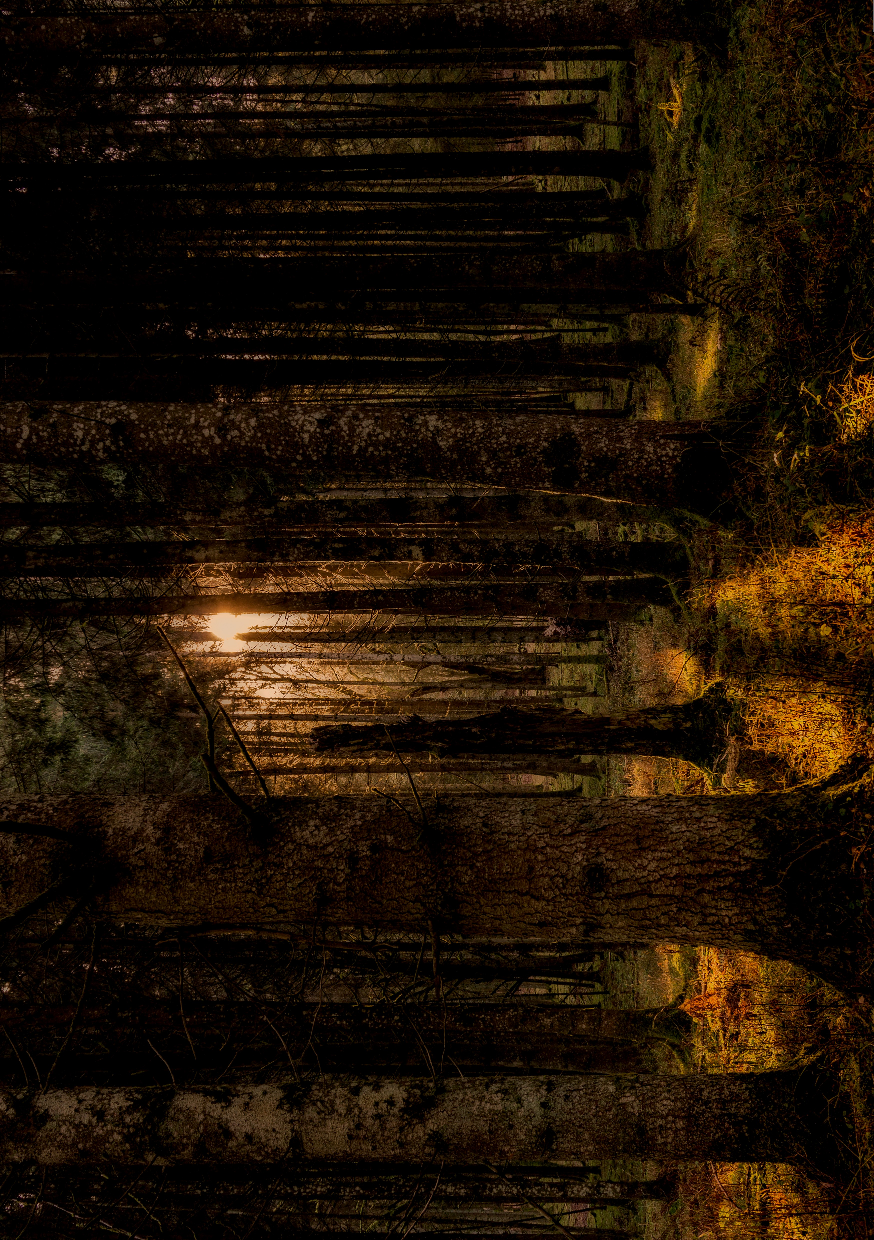
\includepdf[pages=-]{z-include-cygnis.pdf}

»Kennst du Lichtzauber, Ellen?« Es wurde inzwischen dunkel, zumindest im dichten Nadelwald.

»Eine Feuermagierin benötigt keine Lichtzauber, um im Dunkeln zu sehen. Du?«

»Mir fehlen Feuer und Licht zugleich.«

»Wasser?«

»Fehlanzeige.«

»Was kannst du eigentlich?«, fragte die Trollin erstaunt.

»Ich kann Weltsteine schaffen und auflösen.«

Letzteres war wirklich beeindruckend und doch … »Ziemlich nutzlos.«

»Zumindest kann ich wie du den Wald anzünden.«

»Toll. Das war eine meiner einfachsten Lektionen damals. Bei dir funktioniert selbst das nur indirekt. Feuer ist leicht zu erzeugen und schwer zu beherrschen.«

»Ähnliches gilt für Weltsteine«, fand Fnbsrd.

»Nee«, widersprach Ellen sofort. »Die Einstiegshürde ist dort ziemlich hoch. Ein weiterer Grund dafür, dass niemand diese Kunst erlernt. Viel Arbeit für wenig Ergebnis.«

»Mir liegt diese Schule wie dir das Feuer.« Unüblich.

»Du hast vermutlich Schwierigkeiten, einen Zugang zu anderen Formen der Magie zu finden«, mutmaßte Ellen. »Sonst würde ich versuchen, dir zumindest einfachen Funkenflug beizubringen.«

Fnbsrd war offen für Experimente. »Wir können das gerne versuchen. Ich habe Bücher dazu bisher gemieden, um Frustration zu vermeiden.«

»Ein großer Fehler!« Wenig überraschend konnte sie das nicht verstehen. »Aber es geht auch ohne Bücher.« Sie erklärte das Wesen des Feuers in seinen Grundzügen, während unter ihren Füßen der Waldboden vorbeizog. Hin und wieder verlor sie sich in Details, schweifte weit über die Baumkronen ab und kam vor einem Pfeil zum Stillstand.

\textit{Plock.}

Vier langsam, erschrocken und vorsichtig erhobene Hände. Der Pfeil steckte seit drei Sekunden in einem Baum.

»Name, Losung?«

»Scher dich zum Henker und bring uns etwas zu essen«, brüllte Ellen den übereifrigen Wächter an. Der erste Adrenalinstoß wich aufbrodelndem Temperament. »Oder guck zumindest nicht so bescheuert!« Dann riss sie den Pfeil aus dem Stamm, brach ihn mit einer Hand entzwei und zog Fnbsrd mit sich, der noch immer erschrocken den auf sie gerichteten Bogen anstarrte.

Da Ellen vielleicht immun gegen Pfeilbeschuss, wenigstens jedoch nicht ganz durchlässig dafür war, konzentrierte Fnbsrd sich in den nächsten Sekunden darauf, die Trollin zwischen sich und dem Elfen zu halten. Das fing ja gut an.

Die erste Hütte, die sie erreichten, war ihnen schräg abgewandt; davor saßen zwei Elfen und schnitzten faustgroße Holzblöcke zu filigranen Figuren.

»Seid gegrüßt«, rief der Trollgast, »ist Vängä zu Hause?«

Die Elfen erwiderten den Gruß. »Es kann sein, dass sie noch auf Jagd ist«, berichtete einer. »Wenn wir sie sehen, geben wir ihr Bescheid.«

»Danke. Wir sind so lange beim Mutterbaum.«

Fnbsrd nickte den Elfen einmal freundlich zu, trabte passiv seiner Begleitung hinterher und ließ die Umgebung auf sich wirken. Voneinander jeweils mindestens eine Minute Fußweg entfernt waren Hütten im Wald verstreut, mal mehr, mal weniger über plattgetretene Nadeln und zerbrochene Zweige zu erreichen. Echte Wege, selbst Trampelpfade suchte der Städter hier vergeblich. Die Leute von Cygnis achteten den Wald und bearbeiteten ihn nur für ein Mindestmaß an Behausung und Lagerstätten. Hier und dort trugen die Baumrinden spechtlose Löcher.

Der »Mutterbaum« unterschied sich von den anderen Bäumen durch seine Dicke und sein Umfeld: Die dem Mutterbaum zugewandten Äste der direkten Nachbarn waren abgetrennt worden, sodass mittags ein Kreis aus Licht das Siedlungszentrum markierte. Bänke und Tische aus dem, was die Natur freiwillig hergegeben hatte, umgaben sehr unregelmäßig den Kreis. Mal war es ein Baumstumpf, mal ein Stapel aus Zweigen und Moos, aber immer war der Zweck grob erkennbar. An manchen der Tische saßen Lebewesen, größtenteils Elfen, Menschen und ein paar Zwerge; für Trolle und Drachen war die Enge des dichten Waldes offenbar zu unangenehm. Ellen konnte das gut nachvollziehen und fühlte sich wie ein Elefant im Porzellanladen.

Durch das vom Wald gedämpfte Stimmengewirr der Naturkneipe hindurch bot Ellen Fnbsrd einen Platz an. »Hier könnten wir auf Vängä warten. Ich gucke eben nach, ob sie zu Hause ist.«

Wie von den beiden Elfen gemutmaßt, war das nicht der Fall. Ellen kam bald zum Tisch zurück, über einen anderen Pfad als auf dem Hinweg. Der Boden wollte geschont werden.

»Kann ich euch etwas zu trinken bringen?«, fragte ein kellnernder Elf, als beide saßen.

»Für mich ein großes Fass Wasser, bitte.« Ellen rieb sich die Hände und blickte Fnbsrd erwartungsvoll an.

»Äh, ein Krug würde mir genügen.«

»Sehr wohl«, bestätigte der wenig überraschte Kellner schmunzelnd und verschwand in Richtung der nächsten Hütte. Licht schien daraus hervor und Suppe schien darin zu brodeln; das Zischen von Öl in einer Pfanne untermalte das Bild.

Ellen hielt ein paar vertrocknete Kiefernnadeln auf offenen Händen über den Tisch. »Hier, probier mal.«

Fnbsrd nahm mit dem Pinzettengriff seiner rechten Hand eine der Nadeln auf und machte Anstalten, diese zum Mund zu führen.

»Die anzuzünden, meine ich!«

»Hier? Mitten im Wald?«

Ellen lachte tief und zog dröhnend einige Blicke auf sich. »Deinem Talent nach zu urteilen ist der Wald nicht in Gefahr.«

Es entstand dann auch tatsächlich nur ein stinkender Schmorbrand in Ellens Händen, eher rußiger Rauch als sichtbare Flamme.

»Für den Anfang nicht schlecht«, log Ellen. Dabei war das selbst für einen Anfänger ein tölpelhafter erster Schritt. Um diesem Menschen Elementarzauber beizubringen, war unmenschliche Geduld vonnöten.

\begin{center}
∞∞∞
\end{center}

Im späteren Verlauf des Abends stimmten einige der Siedler einen Gesang an. Instrumente, die nur durch Magie einen Sinn ergaben, untermalten den Chor; zwölf Elfen erzeugten Geigen- und Klaviertöne aus Stöcken, Ellen klatschte im Takt. Fnbsrd, der bisher wenig mit Zwergen zu tun gehabt hatte, war überrascht über deren tiefe Stimmen. Der Hauptsänger der spontan entstandenen Band war zwei Köpfe kleiner als der Mensch aus Last Hope und stimmte Töne an, die ein Drache nicht besser ausdrücken konnte. Er sang von dunkler Vergangenheit; eine Menschenfrau lieferte den hohen Gegenpart.

»Kann ich mich zu euch setzen?«, bat ein Elf.

»Klar. Hier sind genug Plätze frei.« Klatsch, Klatsch, Klatsch. »Together for eternity! Das da ist Fnbsrd, ich bin Ellen. Mit wem haben wir die Ehre?«

»Hallo Fnbsrd, hallo Ellen. Föräg ist mein Name. Was treibt euch nach Cygnis?«

»Die Musik«, behauptete Ellen einfach. Sie ließ sich durch Small Talk nicht vom Feiern abhalten.

»Wir warten auf Vängä«, erklärte Fnbsrd. »Und Vängä wartet auf uns.«

»Oh, das wird dauern.« Föräg bestellte sich einen großen Krug Bier – typisch für jemanden, der in absehbarer Zeit nicht mehr rational denken musste. Ellen stempelte ihn gedanklich als ungeeignet für ihre Mission ab und wandte sich wieder der Musik zu.

Fnbsrd entnahm seinem Wasserkrug etwa die Hälfte des Inhalts und blickte dem Tischgast tief in die Augen. Der bekam es kaum mit. \iathought{Weißgrün. Pastellfarbene Naturverbundenheit.} »Wieso?«

Der Bierkrug wurde gereicht und dankend entgegengenommen. Dann blickte Föräg den Menschen an. »Vängä jagt gerne bis in die Nacht hinein.«

»Sympathisch.« Fast frech, jedenfalls aber grinsend erwiderte der Mensch den Elfenblick. »Dabei müssen wir morgen früh raus.«

»Was habt ihr vor?« Ein Zug, ein leerer Krug. Mahlzeit.

»Zwei Schnitzel und noch ein Wasser bitte.«

»Gern.«

Fnbsrd ignorierte die Frage des Biertrinkers einfach. Er tippte Ellen an, die gerade das nächste Lied mitsang.

»Hey dear, won’t you spend another two? One for me and one for you!«

»Hey Ellen. Ellen.«

»Hm?« Klatsch, Klatsch, Klatsch.

»Vängä kommt später!«

»Okay.« Kurzes Nachdenken zwischen den Liedzeilen. Der Kellner witterte Hunger und war sofort zur Stelle. »Fünf Schnitzel mit Pilzen, dazu drei Kartoffeln.« Ein bisschen wenig für den Trollmagen, sagte der Kellnerblick. »Und nach der Vorspeise das Gleiche noch mal.« Schon besser. Grinsend ging die Bestellung an die Küche.

Föräg leerte einen zweiten Krug und erkundigte sich dann erneut nach der Mission. Diesmal unterbrach Ellen ihren Gesang und nahm sich den Elf vor. »Wir gehen in die Hölle. Willst du mit?«

Nach viel zu kurzem Nachdenken hieß es daraufhin, das komme auf die Bezahlung an. Spätestens jetzt hatte sich der Schaulustige disqualifiziert.

»Wir brauchen keine Söldner; die Bezahlung ist ein feuchter Händedruck. Bitte geh zurück an den Kindertisch.«

Der Elf verstand, wenn er verloren hatte. Fnbsrd war mit seinem Abschied zufriedener als mit Ellens Verabschiedung; so machte man sich Feinde. Davon waren gerade gar keine zu gebrauchen. Als der verbal Geprügelte sich in den Wald zurückgezogen hatte, stellte Fnbsrd seine Begleitung zur Rede. »Das war strategisch unklug, bei aller Liebe zum Feuer.«

»Mh«, murrte Ellen. »Strategie ist nicht meine Stärke. Ich räume Steine grundsätzlich erst dann zur Seite, wenn sie mir im Weg liegen.«

»Das wird uns noch früh genug geschehen«, orakelte Fnbsrd düster.


\chapter{Tourner Dans Le Vide}

Als Vängä die Bühne betrat, tat sie das quasi wörtlich. Sie trug ein riesiges silbernes Schwert in einer gläsernen Hülle auf dem Rücken, einen kleinen Handbogen am Gürtel und ein Köcherchen auf der anderen Seite. Ohne Zauberei war damit kaum Wild zu erlegen.

Um ihre Längsachse wirbelnd, bahnte sich die Elfe einen Weg durch die Musikanten, ohne einen davon zu berühren. Das war leichter geschrieben als getan, denn diese tanzten im Takt zu allen Seiten.

»Das ist sie!« Das Klatschen wich beidhändigem Winken. »Hier sind wir.«

Vängä hatte sie längst unter den Speisenden ausgemacht. Nur der Mann in Schwarz war ihr unbekannt.

»Vängä, Fnbsrd. Fnbsrd, Vängä.«

Fnbsrd erhob sich und begrüßte die Elfe erfreut mit Handschlag. »Die Verbündete, ohne die das Unterfangen in die Hose geht.«

»Ah, der Verrückte. Dann sind wir fast vollständig.«

Ellen räusperte sich, was stets wie ein kleines Erdbeben wirkte. »Fast?«

»MAGNUS hat eine Wette verloren.«

Im Gegensatz zu Fnbsrd verstand Ellen sofort, wer nun noch eingesammelt werden musste. Unter dem Mutterbaum schien er sich jedoch nicht zu befinden. Sie sah sich demonstrativ in alle Richtungen um.

»Ja, der hat sich in seiner Hütte versteckt.« Vängä lachte. »Der große Krieger.«

Es kostete die Trollin ein wenig Überwindung, den angebrochenen Schnitzelteller aus den Augen zu lassen, aber das Amüsement abseits des Tisches war anziehend genug für eine Essenspause. »Ich bin gleich wieder da«, kicherte sie donnernd.

Während ihrer Abwesenheit kamen Vängä und Fnbsrd ins Gespräch. Fnbsrd erzählte von seiner Herkunft, verdrückte ein Schnitzel nach dem anderen und erreichte über wasserfarbene Auslassungszeichen schließlich Alpha.

Das war Ellens Stichwort. »Der Held hat eine Sauerei in der Kneipe hinterlassen, das ist nicht feierlich. Irgendein Biest hatte seinen Arm zerfetzt.« Sie übertrieb maßlos und setzte dann den Vierten im Bunde auf einen der Stühle. Das fiel ihr nicht schwer, denn der schmollende MAGNUS war ein Zwerg.

»Moin«, murrte der Rothaarige in seinen Bart. »Ich soll hier einmal die Welt retten. Leider sehe ich nur drei kümmerliche Pfeifen beim Saufen.«

»Hallo MAGNUS, ich bin Fnbsrd.« Die Belustigung war hörbar. »Darf ich dir ein Wasser anbieten?«

»Hmhm.« Nicken. »Wettet niemals mit einer Trickserin.«

»Ey«, protestierte Vängä. »Das lief alles mit rechten Dingen ab.«

»Pff.«

Über die Zeit hinweg wurde klar, dass MAGNUS nicht wirklich unzufrieden mit seiner Situation war. Er machte sich künstlich rar. Mit der Aussicht, früh am Morgen aufbrechen zu müssen, schien er erst richtig wach zu werden. Das war ein Abenteuer nach seinem Geschmack; die Wette war eine Ausrede für Unternehmungen mit Amateuren.

»Welche Magieschule liegt dir am nächsten?«, erkundigte sich Fnbsrd. Aus den Augen war nicht viel abzulesen.

»Alle«, behauptete der Zwerg. Er ließ seine Haare in Flammen aufgehen, löschte sie mit einer kleinen Regenwolke, ließ von dort einen kleinen Blitz in den Tisch schlagen und blies das Feuer aus, ohne seinen Mund zu öffnen. »Einen Topf Erbsen hätte ich gerne. Bitte nicht ziehen lassen, sondern direkt nach dem Aufkochen absieben. Dazu Spargel und wilde Erdbeeren.«

Ellen lachte. »Lass dir keinen Quatsch erzählen. MAGNUS ist inzwischen hunderte Jahre alt und hat mühsam die Grundlagen aller Schulen gelernt. Seine eigentliche Spezialität sind Windzauber. Du müsstest seinen Bogen sehen.«

»Und das alles setzt er für einen Drachen aufs Spiel?«, fragte Fnbsrd noch einmal, als habe er das Prinzip noch nicht verstanden.

»Ich setze stets nur fremde Leben aufs Spiel«, entgegnete MAGNUS. »Und im Gegensatz zu vielen moralischen Weicheiern um dich herum kannst du vielleicht noch am ehesten verstehen, dass ich dabei auch vor Transferzaubern keinen Halt mache.«

»Wer MAGNUS ernsthaft in Lebensgefahr bringt, muss mit übler Notwehr rechnen«, bestätigte Vängä gruselnd seine Worte. »Ich hoffe, du bist nicht ebenfalls so gestrickt.«

»Ich kann gar keine Transferzauber«, behauptete Fnbsrd. Er musste sich notgedrungen korrigieren: »Außer Heilzauber.«

»Für den Anfang ausreichend«, meinte MAGNUS. »Die Welt ist groß, grausam und unnachgiebig. Du kannst dir einen Weg bahnen oder wie diese Erbsen enden.« Der Topf wurde serviert; die Erbsen waren schnell verdrückt. »Oder wie der Spargel.« Gegessen. »Oder die Erdbeeren.« Die auch.

Ob dieser Zwerg als Vorbild taugte, war mit wenig Zweifel zu verneinen. Von Vorteil war jedenfalls, nicht sein Gegenspieler zu sein. Die Bewohner von Pavonis sollten sich warm anziehen.

\begin{center}
∞∞∞
\end{center}

Die fensterlosen Hütten von Vängä und MAGNUS waren magisch angenehm erleuchtet und sogar erwärmt, aber vergleichsweise klein. Fnbsrd übernachtete in einem Gastbett bei Vängä, Ellen passte auf MAGNUS auf. Sagte sie zumindest wörtlich so, was den Zwerg ganz schön auf die Palme und alle anderen zum Lachen brachte.

Vängä war blond, silberäugig von ihrer Liebe zum Wind, nur minimal kleiner als Fnbsrd und trug unter der grünbraunen Tarnkleidung einen Dolch sowie einen schwarzen Büstenhalter.

»Ohne emotionale Abhängigkeiten«, säuselte die Elfin, während sie sich der Jagdkleidung entledigte.

»Oh mein Gott«, murmelte Fnbsrd. \iathought{Will sie mich testen?}

Das Lächeln war recht eindeutig, der Lippenbiss eine überflüssige Vorgabe nicht wirklich vorhandener Schüchternheit. »Schläfst du immer in Jeans?« Sie kicherte.

»Hör mal«, stotterte Fnbsrd, »du hattest deine Jagd heute schon. Mich hat in Last Hope bereits jemand erlegt.«

\iathought{Das war ja fast zu erwarten gewesen}, hieß der gegen eine Eiswand gestoßene Blick. Die Zähne wichen einem Schmollmund. »Nicht einmal die Brille hast du für mich abgenommen«, seufzte die nur noch mit ihrer Unterhose bekleidete Elfendame enttäuscht. Sie sah wirklich bezaubernd aus; ob Aqua je protestiert hätte, stand in den Sternen. Fnbsrd sah in dem Einwand einen Strohhalm, an dem man sich vor dem Ertrinken retten konnte.

»Meine Iriden sind schwarz wie der Abgrund zwischen den Welten«, berichtete der Menschenmann, »und hinter meinen Pupillen lechzt der infrarote Schlund der Hölle. Wer unvorbereitet hineinblickt, bekommt ihr Feuer ins Gehirn gebrannt.«

Das waren recht grauenhafte Aussichten. Die Liebeslust war bald verflogen, auch wenn Fnbsrd sich zu keinem Zeitpunkt bemühte, den Blick von dem Kunstwerk zu nehmen, das der Wald ihm gemalt hatte. Vängä ging mit der Genugtuung zu Bett, dass Fnbsrd länger als üblich zum Einschlafen benötigen würde, weil beide auf eine Decke verzichteten.

\begin{center}
∞∞∞
\end{center}

Der Wecker des Tages war Silberlicht, das auch durch die Sonnenbrille hindurch belebende Wirkung hatte. Es leuchtete gleichmäßig von der Decke, blendete die Elfe vermutlich und gab dem Anblick des gestrigen Abends einen einzigartigen Kontrast.

»Hübsch«, bekannte Fnbsrd gähnend. »Und viel zu früh.«

Die Jägerin war schnell auf den Beinen. Einen kurzen Moment lang spielte der Mensch mit dem Gedanken, mit sanften Schwerkraftzaubern ein wenig Verwirrung zu stiften. »Dein Schmunzeln kommt zu spät«, lachte sie. Das Licht fiel für vielleicht zwei Augenschläge aus, dann befand sich das Schwert wieder auf dem getarnten Rücken. Kurz darauf lag eine Feldflasche in seiner Hand und ein kleiner Rucksack neben seinem Bett.

»Komm nach, ich wecke MAGNUS.«

Hinter ihr fiel die Tür sanft in den Rahmen zurück.

\begin{center}
∞∞∞
\end{center}

Als Fnbsrd mit der Ausrüstung nach draußen trat, erlosch hinter ihm das Licht. Der Pfad zur Hütte des Zwergs war sanft aus dem Boden heraus erhellt; Regentropfen reflektierten das Wegeslicht. Es war weniger heiß als in der Hütte, fast kühl, soweit Fnbsrd diese Temperatur empfinden konnte.

Unter seinen Füßen gab das Laub knisternd, ein Zweig knackend nach. Von Mondlicht war keine Spur zu sehen, auch der Regen erreichte nur auf filigranen Umwegen sein Ziel. Ohne Lichtzauber war eine stolperfreie Fortbewegung unmöglich. Hier lag ein ganzer Baum im Weg – nicht erst seit gestern, der schwach erleuchteten Verfaulung nach zu urteilen.

Ungewollt mit einer zweistelligen Zahl von Pilzen auf dem Gewissen erreichte der Mann aus Last Hope das Wegende. Er klopfte an das Hüttenholz, wurde von MAGNUS tiefer Stimme hereingebeten und zog die Tür vorsichtig nach außen.

»Es ist dunkel, nass und früh am Morgen.« Das war Ellen, die ihre Wächteraufgabe vermutlich auf dem harten Boden verschlafen hatte. Fnbsrd grinste. Des mächtigen Zwerges Hütte war natürlich bettlos.

»Beste Voraussetzungen«, gab MAGNUS sofort an.

»Für Stress und Verderben.« Die Trollin schnippte mit den Fingern und das Licht verdunkelte sich auf ein Drittel des Üblichen. »Bereitet euch auf einen Marsch vor, an dessen Ende nicht zwingend eine Unterkunft steht. Für Proviant ist gesorgt.«

MAGNUS verteilte Nahrungspakete an jeden Expeditionsteilnehmer. Ein großes für Ellen, zwei angemessene für Vängä und Fnbsrd, ein drittes der gleichen Größe für sich selbst. Dann trat er die Hüttentür nach außen und gab den Takt vor. Ellen verriegelte als Nachhut beide Türen mit groben Vorhängeschlössern, vergewisserte sich, dass das Dorf ruhig vor sich hin schlief und trabte dann hinterher. Schwach wie zuvor leuchtete der Boden durch Vängäs Lichtzauber. Hin und wieder tauchte MAGNUS einzelne Punkte in beißend hartes Weiß.

Die beiden Bewohner von Cygnis trugen eigene Kompasse und Landkarten bei sich. Ziel war Pavonis, wo man als Touristengruppe die Höhle des Löwen sondieren und notfalls das ganze Dorf anzünden wollte. Das kam ganz auf den Empfang an.

Während Fnbsrd bereits über die Mittagspause nachdachte, richtete der Zwerg seine leuchtende Aufmerksamkeit auf den neben ihm fließenden Bach. »Guck mal, Fische.« Ab und zu sprang einer heraus. »Fangen und essen?«

»Falls jemand weiß, wie man das macht, gerne.«

Das ließ sich der hundertjährig Erfahrene nicht mehrfach sagen. Bei der Zubereitung wollte Ellen assistieren, doch sie kam nicht dazu. Ein Ruck durchfuhr den Fisch, der daraufhin ein Loch hatte. Die drei Fischer starrten die Wunde erschrocken an, dann erhellte ein Lichtkegel den Morgen. Er spiegelte sich in pastellgrünen Augen und hässlich grinsenden Zähnen. »Das wäre doch nicht nötig gewesen.« Föräg trat heran und griff nach dem Geschenk.

Ellen hatte bereits ihre Faust zu einer passenden Antwort erhoben, als MAGNUS Lichtschein den Rest der Räuber erleuchtete, einen nach dem anderen. Der düpierte Elf von der Außenwache war dabei, der neugierig blickende Mensch vom Nebentisch, selbst der Sänger vom gestrigen Abend erhoffte sich offenbar einen Anteil an der Beute.

»Ich glaube, euer Dorf hat euch verraten«, murrte Fnbsrd. »Wir sind in allerbester Gesellschaft und es sind fünf Bögen auf uns gerichtet.«

Weit mehr als fünf Gegenspieler lachten größtenteils aus der Dunkelheit. Und wo war Vängä abgeblieben?

Nun, da die Karten halbwegs offen auf dem Tisch lagen, gab Föräg dem toten Fisch seine Unterkunft zurück; der Beutel an Ellens Gürtel war deutlich interessanter. Bei aller Bedrohung wagte die Trollin es jedoch, dem Griffel vier kräftige Finger in den Weg zu legen. »Falls ihr handeln wollt, dann nur gegen Vorkasse.« Dann schlug sie Föräg mit voller Wucht ins Gesicht; er folgte dem Fisch bachabwärts.

Fnbsrd, der sich panisch an seiner Mandel verschluckte, verwandelte sich recht abrupt in einen Baum.

In einen Baum. \iathought{Schönen Dank auch}, raschelte es im Geäst. \iathought{Ich bin umzingelt von Mördern und habe wunderschöne Fußfesseln.} Dann schlugen die ersten Pfeile in ihn ein.

Fehlendes Tageslicht war bald kein Faktor der Sichtweite mehr; die dem Dorf angedachte Notfallbehandlung verbesserte Bogen für Bogen, bis das Holz unter der Sehnenlast brach. Den anstürmenden Schwertkämpfer empfing eine Klinge, die seine zerteilte und am Metall keinen Halt machte. Die Fische freuten sich über Vängäs Wiederkehr; das Silberschwert erntete Kerben der Gerechtigkeit. »Wir haben genug Proviant und keine Zeit zum Jagen«, zischte die Jägerin. Eine zweite Nahkämpferin ging zu Boden. »Du?« Nun, jetzt offenbar nicht mehr. Der Rest floh, wie ihn seine panikdurchstoßenen Beine trugen. »Ekelhafter Verrat, so weit das Feuer reicht.«

Für einen Moment brannte still die Vergeltung vor sich hin.

»Wo ist Fnbsrd?«, fragte Vängä dann fast panisch. Sie hatte den Herrn in Schwarz in der Dunkelheit fast vergessen.

»Fnbsrd ist ein Baum«, erklärte MAGNUS und wies auf denselben. »Ist wirklich so.«

»Respekt. Wir sollten die Pfeile herausziehen, bevor die Verwandlung endet«, schlug Ellen vor. Sie begann äußerst vorsichtig damit und formte das Harz wie Pflaster. »Er wollte das so, hat mir ein Wirt erzählt.«

»Schräger Kauz«, fand ausgerechnet der Zwerg. Die anderen grinsten.

\iathought{Ich habe leider keine Ahnung, wie ich diese Form beenden kann}, seufzte das Geäst, unhörbar für die hilfreichen Wesen darunter. \iathought{Vielleicht müsst ihr morgen noch mal vorbeischauen oder Viridia um ein Gegenmittel bitten. Ellen wird ja hoffentlich auf diesen Gedanken kommen.}

»Es kann sein, dass wir in Alpha um ein Gegenmittel bitten müssen«, erkannte Ellen dann glücklicherweise auch. »Fnbsrd hat eine Mandel geschluckt, die ihm dort von Viridia, einer grünen Zauberin am Osttor, angeboten wurde.«

Das waren ja großartige Aussichten, fand Vängä. Andererseits konnte man sich über die blockierten Pfeile kaum beschweren, und ein schwach harzender Baum war einem toten Zauberer vorzuziehen. »Ist das auf deinem Mist gewachsen?«, fragte sie nur. Sie setzte sich bereits in Richtung Alpha in Bewegung.

»Wir hatten das so nicht abgesprochen«, wich die Felstrollin der Frage aus. »Niemand wusste, dass wir überfallen werden würden.«

»Besser früh als nach Stunden des Weges«, fand MAGNUS. »Und der Kollege hat sich ziemlich gut gehalten.« Er klopfte anerkennend gegen den Stamm. »Hat was gut bei mir.«

»Dann ist ja klar, wer läuft«, spottete die Elfe. Natürlich stand das fest, aber es würde nicht der Zwerg sein.

»So schnell der Wind sie trägt«, gab dieser daher recht selbstbewusst und gelassen zurück. »Meine Rückzahlung schreibe ich an.« Fast hätte er etwas in die Rinde geritzt, dann ließ er den Unsinn bleiben. Noch war nicht einmal klar, ob nach einer Rückverwandlung vielleicht doch ein medizinischer Notfall vorlag.

Glücklicherweise nahm die begrenzte Wirkung der Mandel diese Ungewissheit von den Schultern der Gefährten, bevor sich jemand auf Medizinsuche begab. Der Baum wurde so plötzlich zum Menschen, wie er Baum geworden war. Unglücklicherweise mit durchlöchertem T-Shirt und Pfeilwunden.

»Merkwürdig verkrustet«, stöhnte der Ex-Baum. »Ich muss mich erst einmal setzen«, sprach Fnbsrd und fiel um.

\begin{center}
∞∞∞
\end{center}

Der Geruch von frisch gegrilltem Fisch brachte den düsteren Herrn wieder aus dem Zwielicht zurück.

»MAGNUS sagt, du bist in Ordnung«, berichtete Ellen. Sie hob vorsichtig seinen Kopf an und fütterte ihn mit Räucherlachs oder irgendetwas Vergleichbarem. Das Feuer des Waldes war erloschen, ausgeblasen von Wind oder gekühlt durch Wasser, vielleicht beides. Das nasse Holz hatte ohnehin schlecht gebrannt.

Der Fisch tat gut. Die Nachricht auch. »So?« Aus kompetentem Munde?

»Solange du nicht noch irgendetwas feststellen kannst, das mir von außen verborgen bleibt, hast du nur ein paar oberflächliche Stiche abbekommen. Fast wuchtiger als spitz. Immerhin bestandest du aus Holz.«

»Viridia hatte mir dazu nur gesagt, Ärzte würden von einem Konsum abraten.«

»Ärzte sind vermutlich nur neidisch auf deine Langzeitfolgen«, klopfte Vängä ihm sarkastisch vor die Stirn. »Nimm ein bisschen von meinem Brot und komm wieder auf die Beine, wir müssen weiter.« Sie durfte das wohl, hatte sie doch mehr zur Rettung beigetragen als selbst der Baum. Ellen und MAGNUS hielten sich bedeckt. »Eigentlich müssten wir zurück ins Dorf und dort ein bisschen aufräumen, bevor wir einfach von dannen ziehen.«

»Niemand hält dich auf«, entgegnete MAGNUS sanft.

Seufzend steckte Vängä das bachgereinigte, von Feuer desinfizierte und trockengewehte Schwert zurück in die Glashülle. Es glänzte selbst im Bodenlicht wie der Mond. »Niemandem würde es etwas nützen, nicht wahr?«

»Oh, das ist so nicht festgelegt.«

»Es ist aber wahrscheinlich«, mischte Fnbsrd sich ein, »dass es niemandem etwas nützen würde. Lasst uns in Pavonis ein echtes Problem lösen.«

Ellen klopfte ihm auf die Schultern und stieß ihn damit beinahe wieder zu Boden. Schnell zog sie die Hände zurück und grinste. »Das ist die richtige Einstellung.«

Vom schummrigen Silber des Elfenzaubers geleitet ging die Reise weiter nach Nordwesten, die Flüsse abwärts. Das Wasser drohte für weite Strecke ungenießbar zu werden, doch ein Wechsel des Orientierungsbachs kam nicht in Frage: Hier hatte man zumindest einen Überblick über mögliche Verunreinigungen.

Über dem breiter werdenden Gewässer ging die Sonne auf, immer weniger vom Dunkelwald verdeckt und immer steiler die Oberfläche vergoldend.

Als gegen Mittag aus dem Bach ein reißender Fluss geworden war, wagte die Gruppe eine Rast mit Wassernachfüllung. Ellen konnte nicht mit Destillation dienen, aber hohe Hitze in ihren offenen Händen tötete die meisten Keime ohne echtes Abkochen.

»Ist das nicht sehr anstrengend für dich?«, erkundigte sich Fnbsrd.

Die Frau aus Alpha lachte. »Schon lange nicht mehr. Das sind Grundlagen. Dafür brauche ich nicht einmal die Rubine.« Sie griff nach dem Stoffbeutel und ließ einige davon in ihre andere Hand rieseln. Im Sonnenlicht sahen sie besonders schön aus.

»Sind die so wertvoll, dass man dafür seinen Ruf und sein Leben aufs Spiel setzt?«

Ellen schüttelte den Kopf. »Üblicherweise zumindest Letzteres nicht«, berichtete sie mit Unverständnis. »Das kann aber in den Augen eines Diebs ganz anders aussehen. Unehrlichen Menschen drückt man keine Magieverstärker in die Hände. Vielleicht war ihnen tatsächlich der Zugang dazu versperrt.«

»Das ist merkwürdig selbsterfüllend.«

Sie nickte.


\chapter{Ausritt ins Verderben}

\noindent \iaquote{»Mit frohem Mut und in der Hand\\
\noindent Ein Schwert aus kaltem Silber.«}

Es war, als ertönte Musik auf dem letzten Wegstück nach Pavonis. Heldenhafte Lieder, die von Wagemut erzählten, und vom Scheitern, das darauf folgte.

»Mir ist nicht ganz wohl bei der Sache«, gab MAGNUS zu. »Das ist vielleicht ein paar Nummern zu groß für uns.«

»Das hättest du dir vor der Wette überlegen können«, rief Vängä ihm ins Gedächtnis. Der Zwerg brauchte Ausreden, keine Motivation.

»Meine Bedenken sind echt«, beteuerte er daher.

»Was soll passieren?«, fragte Fnbsrd naiv.

»Wir könnten sterben«, murrte Ellen. Dabei war das keine Option. Sie ließ sich durch die Gespräche nicht vom Weg abhalten und lief weiter das steinige Flussufer entlang. »Oder gefangen werden.« Auch keine Option.

»Wir könnten stattdessen einen Drachen befreien und den Zirkus niederbrennen.« Schon besser. Ellen nickte.

»Zunächst sind wir Touristen«, schlug Vängä vor.

Fnbsrd runzelte die Stirn. »Mit Schwertern und Bögen?«

»Pff«, machte Vängä. »Die eigentliche Gefahr geht von Zaubersprüchen aus. Es wäre sinnlos, Touristen ihre dinglichen Waffen abzunehmen. Niemand entwaffnet seine Besucher, weil niemand dazu in der Lage ist.«

Das war so logisch wie verrückt. »Soll das heißen, wir spazieren gleich am helllichten Tag bewaffnet in die Höhle der Löwen?«

»Damit alle Teile dieses Plans erfüllt werden können, sind wir früh losgegangen.« Ellen lachte. »Wir wurden ja auch nur minimal aufgehalten.«

Dem inselbegabten Schwarzmagier wurde seine Verwundbarkeit erst jetzt wirklich bewusst. »Für den nächsten Angriff habe ich keine Mandel parat«, entgegnete er mit Furcht. Verlangsamte er seinen Schritt?

»Wir haben dich nicht als Krieger mitgenommen.« Ellen griff nach seiner Hand und zog ihn nach vorn.

»Klar. Was wäre ein solcher Ausflug ohne Kanonenfutter?« Fnbsrd spuckte in den Kies.

»Das werden wir gleich feststellen«, rief MAGNUS von hinten. »Wir haben nämlich keines dabei. Mach dir gefälligst nicht ins Hemd.«

»Dann verrate mir du doch vielleicht, was ich hier eigentlich mache!«

»Du erfüllst eine Prophezeiung, das muss reichen. Andere tun das ihr ganzes Leben lang nicht.«

Andere hätten ja auch ein längeres Leben, murrte der Mensch mäßig überzeugt und ergab sich seinem Schicksal.

\begin{center}
∞∞∞
\end{center}

Nahe der nördlichen Kartengrenze wurde im Osten eine Struktur sichtbar, die sich vom Horizont brutal abhob. Roher Beton formte eine Drohkulisse, schwarz gefärbte Zinnen lagen wie ein Gebiss auf der Dorfgrenze. Zu allem Überfluss begannen Gewitterwolken, das Geschehen zu überziehen.

»Wir sind da.«

»Magst du vorausgehen?«, bat Ellen.

»Oho.« Die Elfe nickte. Ihre nächsten Schritte wirkten weniger grazil als eisern; die roboterlose Welt ließ eine mechanische Angreiferin auf die Bastille stürmen. Im Schritttempo, mit leeren Händen.

MAGNUS stieß Fnbsrd sanft mit einem Ellenbogen in die Seite. »Man wird uns bereits ausgemacht haben. Dass wir noch leben, ist ein gutes Zeichen.«

Der Angestoßene gab Luft durch die Nase zu hören. »Scherzkeks.«

»Ich beliebe nicht zu scherzen. Die Leute da drüben kennen üble Zaubersprüche.«

»Du auch, nicht wahr?«

»Man wird sehen, wie viel von den Leuten übrig bleibt.«

»Halt«, rief dann jemand aus der Ferne. Vängä tat wie geheißen; hinter ihr kam die Kolonne gerade noch kollisionsfrei zum Stillstand. Zum metallbeschlagenen Stadttor fehlten noch mindestens zwei Minuten. Hörbar war der Befehl nur durch Windmagie.

Schwer gerüstete Ritter kamen ihnen in aller Ruhe entgegen. Zwischen ihren zwei Reihen lief ein grau gekleideter Magiermensch mit langem Zipfelhut auf breiter Krempe. Filz.

»Quo vadis?«

»Pardon?«

»Wer seid ihr, was wollt ihr?«

»Wir sind Nomaden auf der Durchreise nach Arae und möchten einige Monde in der Zivilisation verbringen.« Einfach nur »Tourismus« wäre wohl zu simpel gewesen. Plausibel klang es wohl.

»Eure Namen?«

»Vängä.«

»MAGNUS.«

»Ellen.«

»Fnbsrd.«

»Vermögen?«

»Vorhanden.« Ellen griff demonstrativ nach dem Rubinbeutel. Ihr war jedoch nicht nach Bestechung oder Eintrittsgeld, und das sah man den zusammengekniffenen roten Augen deutlich genug an. Der Magier ließ die Krempe tiefer in die Stirn fallen und nickte erhaben. Aus den Angriffsreihen zu seinen Seiten wurde ein speertragendes Spalier.

»Folgt mir.«

Als die Ritter hinter ihnen lagen, fiel nicht nur Fnbsrd ein Stein vom Herzen, obwohl die Wachen natürlich in ihrem Rücken den gleichen Weg gingen. Niemand sprach ein Wort; der Gleichschritt war laut genug.

Vängä fühlte sich durch den Filzträger ausgebremst, hielt sich aber makellos unter Kontrolle. Der Weg durch das Stadttor war eine Formsache, das Willkommen verkam zu einer Floskel. Die vier Abenteurer bedankten sich freundlich und ließen sich über den grundlegenden Aufbau der Stadt unterrichten. Dann ließen sie die Mauern und das Empfangskomitee endlich wirklich hinter sich.

\begin{center}
∞∞∞
\end{center}

Ein Springbrunnen – einer von sieben gleichen – bot frisches Wasser auf der Hälfte des sternförmigen Weges zum Dorfzentrum. Dankbar füllten die Wanderer ihre Vorräte auf; mit einem Hinterhalt war an dieser Stelle mangels Sinn nicht zu rechnen. Klares Grundwasser füllte die Feldflaschen.

»Wovon sollen wir nachher ein Zimmer bezahlen?«, fragte sich Fnbsrd. »Wirklich von deinen Rubinen, Ellen?«

»Notfalls.« Ellen blickte MAGNUS schmunzelnd an.

»Ich bin nicht zum ersten Mal in einem Blaudorf«, berichtete der Zwerg. Ellen wusste das natürlich, Vängä ebenfalls. Fnbsrd hingegen fielen fast die Augen heraus, als er Messingmünzen und Hologrammscheine seiner Ursprungsstadt in den Hosentaschen erspähte.

»Xenos?!«

»Genug für ein Leben in dieser würgreizauslösenden Festung.« Wertlos außerhalb der von Xenophob unterstützten Dörfer, ein Vermögen darin. Die Tasche ersetzte ein Konto; Karten gab es hier keine.

»Vielleicht hatten die Dorfbewohner es darauf abgesehen«, mutmaßte Fnbsrd.

»Unwahrscheinlich«, widersprach Vängä. »Nun gut, möglich. Aber man lebt nicht in selbstgebauten Hütten im Wald, um mit der erstbesten Raubbeute in ein Königsdorf zu laufen. Unabhängigkeit ist den Lebewesen in Cygnis wichtiger als Gold.«

»Finanziell unabhängig wäre man damit jedenfalls.«

Vängä zuckte mit den Schultern. Das war gehaltlose Spekulation.

»Und wie bist du an das Vermögen gekommen?«, erkundigte der ehemalige Xenobürger sich.

»Glücksspiel«, behauptete MAGNUS einfach. Das war wohl sinnbildlich gemeint und hatte mit Poker wenig zu tun.

\iathought{Transferzauber.} Dieses Wort in MAGNUS Stimme ging Fnbsrd durch den Kopf. Manche Transfers liefen ganz ohne Zauber ab.

»Glücksspiel ist das, was wir hier betreiben«, murmelte Vängä. »Wir sollten uns eine Herberge suchen.«

\begin{center}
∞∞∞
\end{center}

Eine rote Doppelaxt zierte die Tür der Kneipe, in deren Obergeschoss Zimmer vermietet wurden: \iaquote{»Labrys’ Logement«}.

Fnbsrd witzelte, MAGNUS habe hier sicherlich schon einmal gewohnt. Der Zwerg war Pfeilen und Bögen jedoch verbundener als Nahkampfwaffen.

Ellen lächelte. »Sollen wir mal anklopfen?«

»Mir gefällt die Singularität deines Wirs nicht ganz«, hieß es räuspernd von Fnbsrd. »Das letzte Anklopfen hat ein Licht gelöscht.«

»Ich werde die Tür schon nicht einschlagen«, beteuerte die Felstrollin. Am guten Willen zweifelte ja auch niemand. Trotzdem war es Vängä, die stattdessen klopflos den Griff zu sich heranzog. Ein Blick hinein: Die Gesellschaft war geöffnet. Die Tür dann auch recht weit. Solange man nicht gerade Drachengröße besaß, kam man bequem ins Innere. Zufall?

»Moinsen.« Die Barkeeperin, ein von Grünpflanzen überwuchertes Menschengebilde, zapfte gerade ein Maß Altbier in einen Blumentopf.

»Das ist Lola«, murmelte MAGNUS. Versteckte er sich wirklich hinter Ellen?

»Das ist doch MAGNUS!« Einseitige Freude war die schönste Freude.

Hinter Ellens breiten Beinen murmelte irgendetwas, alles habe ein Ende, nur diese Wurst habe zwei.

Lola tat so, als habe sie einen schlechten Witz absichtlich überhört; daran war nur die Absicht vorgetäuscht. Sie grinste. »Was kann ich euch anbieten?«

»Zwei Doppelzimmer und vier große Töpfe Wasser«, bestellte Fnbsrd.

Als MAGNUS daraufhin zischte, ob er das denn auch bezahlen könne, wurde es dem Versteck zu bunt. Die Beine traten zur Seite und das Tresenlicht schien auf die rote Frisur.

»Gern.« Die Schlüsselübergabe war ein Routinegriff mit der linken Hand, die rechte griff nach einer Brille mit recht großen, dünnen Gläsern und Goldrand. »Ich lasse drei große Betten bereitstellen.«

»Vier oder einen Sarg«, zeterte der Zwerg. Die Aufmerksamkeit der Barkeeperin hatte er ohnehin. Grüüüün.

»Drei große Betten und einen Kindersarg.«

Die Pflanzenkrone fing verdächtig an, nach Rauch zu stinken.

»Vielleicht genügt auch eine Abfalltüte. Kommt auf die Zusammenhängigkeit des Inhalts an.« Die namensgebende Waffe lag üblicherweise \emph{hinter} dem Tresen.

»Lola, Liebste«, säuselte MAGNUS aus seiner Glut heraus, »lass uns das bei Gelegenheit gemeinsam mit deinem Leben beenden. Bis dahin nächtigen wir bitte in Frieden.«

»Fein.«

Der spöttische Blick gab Vängä den Rest. Sie kicherte, prustete eher, amüsierte sich hörbar noch für eine ganze Weile.

»Ich glaube, die Dame ist ganz in Ordnung«, urteilte Ellen lächelnd. Sie ließ sich von Fnbsrd einen der beiden Schlüssel weitergeben und begab sich direkt zur Treppe. »Ich komme in ein paar Augenblicken dazu. Bestellt mir was Deftiges.«

Lola hob aufhaltend eine Hand. »Wäre Drache etwas für dich?«

Glaube war Veränderung unterworfen, erste Eindrücke einer Revision. Die Selbstverständlichkeit des Angebots brachte die stolze Riesin gedanklich ins Stolpern. Zum aktuellen Zeitpunkt unter Umständen ein glücklicher Umstand.

Unter den mühsam zurückhaltenden Blicken des Gastquartetts legte Frau Makaberwuchs ein paar Kartoffeln und Reis ins Angebot. »Muss weg. In den nächsten Tagen gibt es vermutlich Nachschub.«

»Nachschub«, wiederholte Fnbsrd stimmlos aus der Kehle heraus.

»Der Seher sagt, in ein paar Tagen kommt wieder einer vorbei, um seinen Artgenossen zu befreien.«

»Praktisch«, rotzte Ellens Gehirn so ehrlich wie möglich über die Zunge. Stufe, Stufe, Stufe. »Ich bevorzuge Wild.« \iathought{Wie jede redliche Intelligenz.} »Aber davon gerne viel.«

Die Barkeeperin zuckte mit den Schultern. »Wer neu im Dorf ist, verkennt oft dessen Qualitäten«, erklärte sie den anderen dreien. »Bitte nehmt Platz.« Sie zeigte lächelnd in die Raumecke, in der ein gemütlicher breiter Tisch an einer gewinkelten Polsterbank und zwischen schön verzierten Stühlen stand.

Die Stühle blieben an ihrem Platz, da niemand mit dem Rücken zum Raum sitzen wollte. Dafür erwies sich die Eckbank als sehr bequem. Fnbsrd und Vängä platzierten sich der Bar gegenüber, MAGNUS in größtmöglicher Entfernung seitlich dazu. Für Ellen blieb mehr als genug Fläche an der Wand.

\begin{center}
∞∞∞
\end{center}

Das Barpersonal bestand aus zwei Personen: In der Küche fabrizierte irgendjemand namenlose Rohwaren zu exquisit klingenden Gerichten, in der Bar verteilte Lola Speisekarten und Ergebnisse.

Ellen genoss auch, oder gerade, ohne Drachenanteil den vegetarisch wirkenden Teil des Angebots. Wo eine entfernte Form von Kannibalismus zur Kultur erhoben war, stach die Wildesserin durch Mäßigung hervor. Ihrem ansonsten unstillbaren Appetit standen drei Mägen gegenüber, auf die Begleitumstände geschlagen hatten. Man befand sich schmatzend in der Hölle und mit eineinhalb Beinen tief im eigenen Grab.

\iathought{Leichenschmaus im Voraus}, sinnierte Fnbsrd düster vor sich hin. Auf seinem Teller lieferten sich Erbsen eine Flucht vor der Gabel.

»Noch einen Teller?«, fragte Lola freundlich.

»Zwei sind vermutlich noch drin.« Die Felstrollin nickte; der gerade geleerte wurde umgehend ausgetauscht. Über mangelnden Service konnte man sich in Labrys’ Logement nicht beklagen.

»Darf ich euch noch Getränke anbieten?«

Fnbsrd blickte in seinen Blumentopf. Im Rest des Inhalts spiegelte sich alles, was Licht hineinwarf.

\begin{center}
∞∞∞
\end{center}

\iaquote{»Wer mit Ungeheuern kämpft, mag zusehn, dass er nicht dabei zum Ungeheuer wird. Und wenn du lange in einen Abgrund blickst, blickt der Abgrund auch in dich hinein.«\\
\noindent – Friedrich Nietzsche: Jenseits von Gut und Böse}

\begin{center}
∞∞∞
\end{center}

»Nanu, was war das?«, fragte Lola verwirrt.

Fnbsrd schüttelte sich. »Für mich noch ein Wasser, bitte. Gerne in einem größeren Topf, falls vorhanden.«

»Gern.« Der Blick wanderte zu Vängä. Die nickte und hielt Zeige- und Mittelfinger empor. »MAGNUS?« Drei.

Während die Barkeeperin sich lächelnd zur Küche begab und die Wünsche weitergab, sah insbesondere Vängä ihren Sitznachbarn etwas schräg an. »Ich hatte gerade das Gefühl, ein Riss habe sich durch das Gefüge der Welt gefressen. Recht plötzlich.«

»Das kommt manchmal vor«, tat MAGNUS den Eindruck als Alltäglichkeit ab. »Die Welt verhält sich manchmal, als bestünde sie aus Papier. Manche behaupten, sie könnten das alles von außen erfassen und unser gesamtes Sein wie ein Buch in den Händen halten.«

»Deiner Tonlage nach haben diese Erzählungen nur rudimentären Wahrheitsgehalt«, schloss Ellen.

»Das mag sein; der eigentliche Punkt ist: Wir können ohnehin nichts daran ändern. Nenne es Defätismus oder pragmatisch, versuche dich darüber hinwegzusetzen und verschwende Lebenszeit.«

»Ein geringer Preis für eine Chance auf Weltkontrolle, nicht?«

»Tendenziell nicht, weil niemand dafür genug Zeit besitzt. Außer den Königen natürlich …«

»… und selbst die sind bisher daran gescheitert?« Nun bekam Fnbsrd doch Appetit; die Erbsen wurden fast unbewusst dezimiert. »Ich brauche mehr von dieser Soße.«

Lola widerstand der möglicherweise absichtlich gestreuten Versuchung, daraufhin direkt das Gewünschte zu bieten. Sie erkundigte sich erst eine Weile später nach Wünschen und brachte dann eine neue Ladung Erbsen mit viel Rahmsoße und Pilzen an den Tisch.

Zum Nachtisch gab es Grießbrei mit Zimtpulver und geriebener Zitronenschale. Das sollte wohl gesund schmecken; lecker war es ohne Frage.

»Die Rechnung geht auf mich«, bot MAGNUS dann großzügig an. »Ellen kann ja das Abendessen bezahlen.«

»Scherzkeks«, zischte diese sofort.

Die Übernachtung wurde bei dieser Gelegenheit im Voraus mitbezahlt. Lola bedankte sich für das üppige Trinkgeld und gab den Reisenden organisatorische Hinweise mit auf die Zimmer.

\begin{center}
∞∞∞
\end{center}

»Zwei große Betten.« Die Felstrollin war vorangegangen, öffnete präsentierend die Tür und wies so stolz in den Raum hinein, als habe sie das Mobiliar selbst aufgestellt.

»Die müssen längst dort gestanden haben«, murrte MAGNUS halb schmunzelnd. Er trat ein und blickte sich um. »Lola hat eine große Klappe \emph{und} ein großes Herz.«

»Für Humanoiden.« Ellen folgte und schloss die Tür hinter sich.

»Ja, das ist bitter. Es steht dem König in den Namen geschrieben und bedrückt mich bei jedem Besuch. Wer sich hier niederlässt, hat üblicherweise die eine oder andere speziesistische Macke.«

»Ist es nicht Heuchelei, wenn wir als Fleischesser das so abtun?«

»Ich esse kein Fleisch von Intelligenzwesen«, entgegnete der Zwerg in temporärem Missmut. »Die Leute in der Stadt haben inzwischen Ersatz gefunden, komische Pillen und künstliche Pflanzen. Wir sind auf die Nährstoffe angewiesen. Außerdem halten wir das Vieh nicht in Massen.«

»Mir sagte einmal jemand, es gebe durchaus Diskussionen darüber, was ein Intelligenzwesen denn besser mache als ein Tier. Es gibt da ja einige Gestalten …«

MAGNUS nickte heftig. »Ethik, ja. Schwierig. Wir blasen uns als Moralapostel ganz schön auf.«

»Du hast aber keine echte Antwort darauf, nicht wahr?«

»Du etwa?«

Ellen sog tief und langsam die Luft ein, bis sie gefühlt die eineinhalbfache Breite erreicht hatte. MAGNUS wusste, dass es ihr dabei nicht darum ging, größer zu wirken. Im Kontext der Aufgeblasenheit hatte es dennoch eine gewisse Komik. Dann entwich die Luft durch die Nase; der große Körper krümmte sich fast. »Ich wollte gerade sagen, im Zweifelsfall geht es um mein eigenes Überleben. Das ist legitim.«

Lächeln und Verständnis standen in undefinierbarer Iridenfarbe, von nachsichtiger Mimik umgeben, der unvollständigen Argumentation entgegen. Dann blickten sich die beiden ungleichen Zimmerpartner lächelnd an. »Man könnte meinen, dir bereitet das gerade Schmerzen.«

»Seelisch vielleicht.«

»Wohl dem, der eine Seele besitzt.« MAGNUS grinste üblen Sarkasmus aus der Tiefe. Das waren die Worte des Tages.


\chapter{Skyfall}

Der Abend leuchtete rot wie das Feuer in Ellens Augen, unsichtbare Seelentränen auf Selen, rote Iriden um große schwarze Kreise. Irgendwo in der Ferne stand der Nabenberg im Nebel, dessen drei Talstädte längst keine eigenen Kriege mehr führten. Der eigentlich unabhängig davon arbeitende Mond ging klischeehaft auf der anderen Seite auf.

Im Zentrum des fremden Dorfes umgab rautenförmig ein Park einen See. Die Botanik verdeckte die Hässlichkeit der Dorfmauern, wenn man Wohlwollen mitbrachte. Weniger zentral lag das Silber in Ketten.

Das Quartett hatte sich für diesen Tag gegen einen Besuch des Drachenkäfigs entschieden. Man sah aus der Ferne genug davon, um einen ersten Adrenalinstoß auf sich wirken zu lassen und den weiteren Untergang des Dorfes zu planen.

»Es ist schön hier«, behauptete Fnbsrd.

»Ja, hier kann man eine Weile bleiben«, stimmte Vängä zu. \iathought{Ein Leben lang.}

MAGNUS ließ sich als Erster auf einer hellen Holzbank nieder; die anderen gesellten sich zu ihm. Der Weg lief im Kreis, die Bank war über den See hinweg gegen Westen gerichtet.

»Arae ist noch weit entfernt«, laberte Ellen. »Wir werden das Wasser brauchen.«

Stumpfes Nicken umgab sie von beiden Seiten. Vängä erzählte, es sei immer gut, Vorräte dabeizuhaben.

Als der Abend der Nacht gewichen war, wiesen Laternen den Heimweg. Die damit verbundene Automatisierung wäre den Leuten aus Last Hope ein Gräuel gewesen, bemerkte Fnbsrd. Machte sich Heimweh bemerkbar? Vängä lächelte ihm aufmunternd zu.

Der für die Ferne ersehnten Rückkehr stand vorerst Fensterlicht aus Labrys’ Logement bevor. Ellen durfte vorsichtig am Türgriff ziehen und die Tür gab sanft den Weg frei.

»Na?«, rief Lola von der Theke. »Platz für ein Abendmahl?«

\iathought{Lustig, dass sie das sagt.} »Gern, ja.« MAGNUS vermied direkten Blickkontakt und nahm seinen vorherigen Eckenplatz wieder ein. Ellen war zur Stelle, Elfe und Mensch folgten mit gestiegenem Appetit.

»Belegte Brote mit Gurken?«, bot die Wirtin an. »Dazu natürlich vier Wasser.«

Alle blickten sich kurz um und nickten dann.

»Kommt sofort.«

\iathought{Man muss wirklich aufpassen, das Beißen bei all der Fütterung nicht aus den Augen zu verlieren}, sinnierte Fnbsrd stumm in sich hinein. \iathought{Lola umgarnt uns ja regelrecht.}

Den anderen gingen ähnliche Gedanken durch den Kopf. Einige schwere Entscheidungen standen bevor.

»Fern im Süden gibt es ein Land mit Straßen aus Gold«, erzählte MAGNUS dann ungefragt. Eine Geschichtenstunde stand bevor, und die kam gar nicht ungelegen. Die anderen hingen an seinen Lippen, auch Lola hielt sich sicherlich nicht die Ohren zu. Die eine oder andere Anekdote zauberte ihr ein schwer verdeckbares Lächeln ins Gesicht. Eine Etage oberhalb schlief der Koch den Arbeitstag aus; an Nebentischen boten fremde Gespräche eine milde Geräuschkulisse. Hin und wieder schien es, als habe der Zwerg die ganze Aufmerksamkeit der Kneipe gebucht.

»Und wofür benötigte der Blinde die Kerze?«, fragte Vängä an einem Punkt neugierig nach. Offensichtlich war die Lösung nicht.

»Um gesehen zu werden«, erklärte der Erzähler bereitwillig. »Zum Verhängnis wurde ihm nur, dass sie unbemerkt ausging.«

\begin{center}
∞∞∞
\end{center}

Die Holztreppe knarrte unter Fnbsrds Füßen, was in der Dunkelheit unabhängig von der Stille besonders unangenehm auffiel. Schritt für Schritt in schwarzen Socken: Wozu eigentlich? Toiletten gab es auf den Zimmern.

Die Tür nach draußen war stets geöffnet, die Stadt für ihre Sicherheit bekannt. Je nach Quelle und Art der Sicherheit, philosophierte der Nachtwanderer, bot sich ein Türschloss eigentlich besonders an. Dieses war aber nicht vorhanden.

Mondlicht und Laternen, letztere mit Entfernungsvorteil, ersteres schöner, erleuchtete die Straßen. Die Wege, musste man sagen. Den Pfad. Das alles war auf das Zentrum ausgerichtet, die Gaststätte vielleicht halbwegs im Südwesten.

Ohne Schuhe machte sich der Kies bemerkbar. Eigentlich angenehm, wenig spitz.

Der junge Mann, in dessen Kopf häufig Musik spielte, genoss die unübliche Lautlosigkeit. Jeder Atemzug war ein Genuss.

Merkwürdigerweise erschrak er nicht darüber, dass auf einer Bank neben der Kneipe die Elfin aus seinem Zimmer saß und nicht nur ohne Schuhe das Mondlicht tankte. Sie musste während seines kurzen Spaziergangs lautlos dort erschienen sein, was für eine Windmagierin sicherlich keine Hürde darstellte.

\iathought{Du hier?}, fragte der Blick.

Die Elfe lächelte. \iathought{Das Gleiche könnte ich dich fragen}, antwortete ihrer.

Nächtliche Begegnungen mit Frauen, die mehr oder weniger offen Interesse zeigten, schienen außerhalb der Stadt zum Alltag zu werden. Vängä spielte mit seinen Gefühlen ein windig Spiel und bezog daraus ihre Genugtuung.

\iathought{Diesmal lasse ich nicht sieben Jahre vergehen, bevor ich wieder ein Haus betrete}, schwor sich der Mensch. Er schenkte Vängä einen langen, genussvollen Blick und ein Lächeln, bevor er in die Unterkunft zurückkehrte.

\begin{center}
∞∞∞
\end{center}

»Aufstehen«, dröhnte Ellen von der Seite. Sie hätte ihm genauso gut mit einem Hammer an die Stirn oder an seinem Ohr gegen eine große Turmglocke schlagen können. MAGNUS wehrte sich weniger akustisch, und Ellen ertrug es in üblicher Dickhäutigkeit.

»Ich werde mich nie daran gewöhnen, von einem Troll aus dem Schlaf brutalisiert zu werden.«

So leise, wie sie konnte, flüsterte Ellen daraufhin, das sei auch nicht als Dauerzustand geplant.

MAGNUS wurde sich morgendämmernd darüber bewusst, dass in Cygnis noch eine Rechnung einzutreiben war. Vielleicht würde er sich ein neues Heimatdorf suchen; sein altes Land hatte die Tore hinter ihm geschlossen. »Du bist im Bad fertig?«

Ellen nickte. »Quasi.«

»Dann werde ich mir das jetzt reservieren.« Aus Prinzip.

\begin{center}
∞∞∞
\end{center}

Lolas Frühstück war königlich, das Mittagessen kaiserlich, Brot in Aussicht. Zuvor gab es ein Missionsziel zu besichtigen.

Jede Ausrede dafür nahm die Gastgeberin einfach vorweg. Sie wies die vermeintlichen Touristen auf die Hauptattraktion des Dorfes hin, als müsse man das Verbrechen unbedingt gesehen haben. »Die nächste Fütterung ist um sechzig. Wenn ihr jetzt losgeht, könnt ihr es gut schaffen.«

Innerlich kotzend bedankte sich jeder ganz höflich und verließ das Haus.

Fnbsrd schluckte seinen Redebedarf vorerst herunter. Man wusste nie, wer von den Gesprächen Wind bekam. MAGNUS überbrückte das Schweigen mit weiteren Belanglosigkeiten; seine Begleiter stimmten dankbar in den Small Talk mit ein. Dann kam der hausgroße Käfig neben Häusern in Sicht. Würfelförmig, allseitig vergittert.

»Was ist das denn für ein Material?«, wagte der erneut in Schwarz Gekleidete zu fragen.

»Titan mit Aluminium und Vanadium«, schätzte MAGNUS. Das brachte ihm einige verdutzte Blicke ein. »Glaube ich.«

»Langsam wirst du mir unheimlich«, murmelte Vängä. Fnbsrd nickte.

»Das ist einfach nur das, woraus \emph{er} den Käfig gebaut hätte«, ordnete Ellen die Materialprüfung als wenig magische Behauptung ein.

»Ich baue keine Käfige«, murrte MAGNUS ausweichend.

»Wie dem auch sei: Das muss der Drache sein.« Vor dieser Untertreibung zog selbst der große Analyst gedanklich anerkennend den Hut. Der schuppige Riese glänzte silbern im Sonnenlicht, was dafür sprach, dass es sich um ein fliegendes Wesen handelte. Drachen ohne Windmagie konnten in etwa so gut fliegen wie Pinguine, und zum Erheben eines schweren Drachenkörpers über die Wolken war mehr als nur ein Wochenlehrgang über Wind erforderlich.

Vängä betrachtete staunend den schlafenden Gefangenen. »Eine Trophäe.« So grausam wie selten.

»Dort stehen nicht nur Fütterungszeiten«, bemerkte Fnbsrd als Erster. Die anderen hatten das Informationsschild nicht genauer betrachtet, weil sie die näheren Umstände kannten.

»Richtig«, bestätigte Ellen daher schon nach einem kurzen Blick. Sie zog das »G« in die Länge, was auch ohne »ch«-Laut erstaunlich hörbar gelang. Man konnte die gedachten Auslassungszeichen förmlich hören.

Dort standen nicht nur Fütterungszeiten, mit Betonung auf dem ersten Wortteil.

Vängä wies vorsichtig umschreibend darauf hin, dass der Drache zu festgelegten Zeiten die Gelegenheit erhielt, Auskunft über den angeblich von ihm versteckt gehaltenen Schatz zu geben. Und darauf, dass es mehr Gründe als Böswilligkeit und absichtliche Irreführung dafür gab, dass tatsächlich Orte genannt wurden, an denen sich dieser befinden sollte.

\iathought{Wer nicht verraten kann, was nicht existiert, steht in manchen denkbaren Situationen vor einem schmerzhaften Dilemma.} Fnbsrd begriff und fror stärker, als der kommende Winter es je vermocht hätte. \iathought{Besonders nach einer Prüfung der Antwort.}

»Großartig, nicht wahr?« Ein älteres Paar Menschen stand bewundernd vor dem Käfig. »Ich hoffe, er schweigt noch für eine Weile.« Die Bewunderung galt nicht dem Lebewesen.

\iathought{Wo zur Hölle sind wir hier gelandet?}

Die Holzhammerlösung, das ganze Dorf dem Erdboden gleichzumachen, wurde mit dem Verhalten jedes Dorfbewohners attraktiver. Wem die Gruppe auch begegnete: Alle hielten die Tradition mit Leidenschaft hoch.

\iathought{Und der König hält seine schützende Hand darüber}, überlegte Fnbsrd. \iathought{Es spielt ihm in die Karten.} War es weise, derart bemerkbar auf das politische Spielbrett zu treten? Es bestand eine reale Gefahr von Racheschlägen gegen sein Heimatdorf, und es waren bereits zu viele Lebewesen durch Angriffe auf Last Hope gestorben.

Zumindest gab es eine Möglichkeit, die Leben der Pavoner zu bewahren und eine Prophezeiung zu erfüllen. Fnbsrd nahm sich vor, den Plan erst im letzten Moment zu offenbaren, wenn lauschende Ohren kein Problem mehr darstellten.

\begin{center}
∞∞∞
\end{center}

Der Drachenfütterung als alltägliches Ereignis wohnten nur wenige Interessierte bei. Zwei Familien integrierten sie in ihren Tagesausflug; anderntags gab es Klassenausflüge voll Propaganda. Wirklich spannend oder gar obszön war sie für niemanden im Dorf. Man beglotzte gemeinsam die fortwährende Versklavung eines Intelligenzwesens.

»Aufwachen!« Mehr ein Befehl als eine Aufforderung; der silberne Drache gehorchte in erlernter Hilflosigkeit. Zumindest wirkte er so, als habe er Fluchtpläne längst aufgegeben.

Eine unter weniger widrigen Umständen dem Begriff »Tierpflegerin« entsprechende Wärterin beaufsichtigte die Arbeit ihrer Assistentin. Futterklumpen, graubraune Energie mit Vitaminen, vielleicht gnadenhalber mit Aromen versehen. Vermutlich nicht. Der Drache erhielt sie über eine rostige Eisenrutsche, die Menschenhände und Drachenmaul trennte, und er aß sie als geringstes Übel gegenüber Hungertod und Qualen. Ein Kind klatschte, als habe ein Hund ein Kunststück vollführt. Nicht böswillig, aber dumm.

Neben der fest montierten Rutsche befand sich ein weniger verrostetes Schloss. Hier hatte man nicht am Material gespart: Wie die Gitterstäbe bestand es aus einer Titanlegierung. Weiter unten hing ein gleiches Exemplar an einem zweiten Querbalken. Die Tür war groß, dick und stabil. Ein Drache passte hindurch, aber kein Drache kam hindurch.

Als die Fütterung beendet war und die Zuschauer weitergingen, schloss sich das Quartett dem Rest an. Um Häuserecken an Hinweistafeln vorbei, angebliche weitere Sehenswürdigkeiten im Mindestmaß bewundernd, kehrte die Gruppe zur bekannten Parkbank zurück. Dort verbrachten Vängä, Ellen, MAGNUS und Fnbsrd ihre Zeit mit inhaltsleeren Unterhaltungen und Diskussionen über erfundene Probleme.

\begin{center}
∞∞∞
\end{center}

Auch an diesem Abend weihte MAGNUS seine Gefährten in die Geheimnisse der Weltgeschichte ein. Dazu gab es Brotsuppe – wenig kreativ, aber recht nahrhaft. Mit Brot.

Des Nachts wiederholte sich ein introvertiertes Ritual, Treppenstufen knarrten. Mondlicht erhellte die Dunkelheit ausschnittweise. Fnbsrd starrte den Felsbrocken an, lobte sich die Sonnenreflexion, oder was auch immer in dieser Welt der Mond von sich gab. Es war nicht einmal klar, ob es derselbe Mond wie in der Vornacht war.

»Man hätte sich darüber mehr Gedanken machen können«, murmelte Fnbsrd. Dann ging er weiter den Kiesweg entlang. »Vieles ist nicht richtig durchdacht.«

Die erste ihm auf dem Weg begegnende Seele war in dieser Nacht keine Elfe. »Es grüßt«, nun, »Ventosus, der Windmagier.« Auch mit gezogenem Filzhut eine recht undurchsichtige Angelegenheit.

Fnbsrd blieb äußerst vorsichtig und ohne hektische Bewegungen an der Kreuzung stehen. »Fnbsrd. Sehr erfreut.« Sehr reserviert? Nein, fast freundlich.

»Ich sehe, wir teilen eine Vorliebe für Nachtspaziergänge. Mir tut die stille Luft gut, Ihnen das Dämmerlicht?«

Jedes Wort wollte wohlbedacht sein. Bereits die unverfänglich wirkende Frage steckte voller Fettnäpfchen. »Gewiss«, bestätigte der Dunkelgast. Eine minimale Irritation durfte durchaus hörbar sein, und die Wahrheit war leicht über die Zunge zu bringen. »Ich fühle mich der Nacht mitunter verbundener als dem Tag.«

»Sie sind mir sympathisch, Fnbsrd«, behauptete der Silbermagier. Er drückte seine Hutkrempe leicht nach oben; seine silbernen Augen spiegelten das milde Leuchten. »Daher möchte ich Ihnen ein Angebot unterbreiten.«

\emph{Nun} schrillten die Alarmglocken. Der Weg war zwar keine Einbahnstraße, aber Rückwärtslaufen blieb ein Wunsch. Der Mann in Schwarz räusperte sich tief. »Inwiefern?«

»Zehntausend Xenos für die Elfe.«

In Fnbsrd starb etwas, und es tat das recht sichtbar durch jeden Sonnenschutz hindurch. Die Stimme war mindestens Teil des Sterbenden; jede Hoffnung war todgeweiht.

»Zehntausend Xenos und eine silberne Drachenschuppe.«

Gestorben. »Ventosus, welche Rolle spielen Sie in diesem Dorf?« Wo Leser zu Wasserflaschen griffen, kratzte im Roman unheilbar der Hals.

»Man hat mich zum Bürgermeister erkoren«, erklärte Ventosus, als stünde er an einem Basartisch. Die Stimme war zeitgedämpft und wurde von Blättern der umliegenden Bäume geschluckt, doch das fiel in der Stille kaum auf. »Ich kommuniziere für das Dorf mit den blauen Ministerien und Dorfgästen.«

»Seit wann tun Sie das?«

Ventosus grübelte. »Gut drei Jahre dürfte das her sein. Mein Vorgänger wurde in die Verwaltung des Blautals befördert und hat keine Zeit mehr für Lokalpolitik.«

»Es handelt sich also um ein offizielles Angebot.«

»Nein, es handelt sich um offenen Machtmissbrauch.« Das war nicht die Stimme des Magiers. Der windige Händler drehte sich anteilsweise freiwillig im Halbkreis. Hinter ihm stand eine Elfe mit Silberschwert.

»Oh, guten Abend«, stieß er dann tief und rau hervor. Er wirkte wenig beeindruckt. »Darf ein Bürgermeister nachts keine Geschäfte tätigen?«

»Das kommt auf deren Inhalt und die gewünschte Dauer seines Lebens an«, knurrte Vängä.

Ventosus winkte lachend ab. »Die ganze Welt ist käuflich. Alles hat einen Preis.« Dann ging er quer über die Wiese davon, fühlte sich sichtbar unsterblich und war bald darauf im Dunkeln verschwunden.

»Es gibt Gesellschaften mit Normen, die wir nicht verstehen«, flüsterte Fnbsrd.

»Es gibt Normen, die wir nicht dulden müssen«, erwiderte Vängä, für ihren Adrenalinpegel recht sanft. »Unsere Anwesenheit in diesem Dorf war eine bewusste Entscheidung.«

»Ist das nicht anmaßend?«

»Ungefähr so anmaßend wie Pfeil und Bogen bei einem Raubtierüberfall. Fragwürdig wie ein Keks.«

Die beiden kehrten unbehelligt und unbemerkt in die Gaststätte zurück. Mit Ärger im Nacken schlief jeder für sich gleich schlecht.


\chapter{Don’t Say a Word}

Bestärkt durch die Ereignisse der Nacht, beschleunigt durch das Gefühl nahenden Unheils, wurde eine selbsterfüllende Prophezeiung ihrer Erfüllung entgegengeschoben. Zum Frühstück gab es Rührei mit Pfeffer.

»Viel Pfeffer« erbat Fnbsrd.

Lola fühlte sich herausgefordert und kippte die halbe Pfefferdose über das Ei. »Wohl bekomm’s!«

\iathought{Sprich kein Wort, dann bleibt meine Seele gesund. Dein Nächstes wird kein Tischgebet.} Fnbsrd verschlang den geeiten Pfeffer wie eine Süßigkeit; selbst Ellen war beeindruckt.

»Pfeffer wird üblicherweise erst am Tisch hinzugefügt, da er bei Hitze bitter wird«, erklärte MAGNUS.

»Dort stand aber nicht mehr genug zur Verfügung«, stellte Vängä belustigt fest. Sie wog den Pfefferstreuer hin und her und stellte ihn wieder ab.

Ähnlich verlief das Mittagessen; zum Abendmahl kehrte die Gruppe nicht zurück.

\begin{center}
∞∞∞
\end{center}

Tiefrot durch Sonnenstrahlen erleuchtet war der Drache von einem goldüberzogenen Wesen kaum zu unterscheiden. Von Vängäs Windzaubern unterstützt praktisch lautlos hatte sich Ellen dem Käfig genähert, kniete nieder und griff nach dem unteren Schloss. Kein Geräusch ertönte, niemand sprach ein Wort.

Der Abend der Wahrheit war angebrochen. Das Metall auch. MAGNUS kannte Ellens Stärke und war dennoch stets aufs Neue von ihrer Fähigkeit beeindruckt, selbst Titan mit den Händen zu zerdrücken. Vielleicht, redete er sich ein, half er dabei mit unbewussten Zaubern nach. Die Zuschauer wetteiferten jedenfalls mit dem Schlossgegner.

Mit mindestens einem Ohr am Käfig konnte der Drache hören, was in der Windstille den anderen verborgen blieb: Das untere Schloss zerbrach, die Minuten des oberen waren gezählt.

Drachen wuchsen und lebten Jahrhunderte lang. Dieser hatte in seinem Leben einiges erlebt, aber noch keine Befreiung aus einem Käfig. Fast hatte er freundliche Worte verlernt; fast fehlten Synapsen zur Verarbeitung des dort Geschehenden.

Als Ellen von einem brutalen Windstoß zur Seite geboxt wurde, riss sie den Hauptteil des Vorhängeschlosses mit sich. Der Käfig war nur noch von Riegeln verschlossen, die sich von innen jedoch kaum öffnen ließen.

Der ohnehin nicht helle Himmel verdunkelte sich; ein Hurrikan zog auf. MAGNUS flog mit Fnbsrd zwanzig Meter in Ellens Richtung gegen eine Hauswand; Vängäs Schwert gehorchte dem Elfenwind nicht mehr.

Die sich langsam aufrappelnde Felstrollin starrte ein Wesen in grauem Filz an, das die Situation nach seinen Vorstellungen bereinigte. Es hatte sogar Ersatzschlösser dabei, und mit ihrer eigenen Klinge vor der Nase wirkte die Blondine ein wenig hilflos.

»Vängä, richtig?« Der Bürgermeister stieß blind ein Schloss durch den Riegel. Er vergewisserte sich einer rückendeckenden Windwand, ohne lange den Blick abzuwenden. »Ihr seid hierher gekommen, um unseren Drachen zu stehlen.« Er lachte einmal kurz laut auf. »Durchsichtig und naiv.«

»In jeder Hinsicht deinem unwürdigen Gehabe überlegen«, stieß sie zwischen den Zähnen hervor. Eine Windböe brachte sie zum Schweigen.

MAGNUS wusste, wann man den taktischen Rückzug antrat. Ellen und Fnbsrd benötigten einen zweiten Windschlag, um zur gleichen Erkenntnis zu gelangen.

»Wohin?«, keuchte Letzterer.

Irgendjemand griff nach seinem Kragen. »Weg. Aber weder in die Gaststätte noch aus diesem Dorf hinaus.« Das Trio stolperte mit entsetzten Rückblicken in Deckung. »Die Stadtwache muss bereits unterwegs sein und hat alles umstellt.«

»Bist du dir sicher?«, fragte Ellen zweifelnd.

»Du meinst, man möchte drei Viertel fliehen lassen?«

Beide nickten.

»Das wäre ein weiterer Grund, hierzubleiben.«

\begin{center}
∞∞∞
\end{center}

In die momentane Planlosigkeit mischte sich zusätzliche Überraschung: Die Tierwelt floh mit Verspätung und zielgerichtet gen Süden vor dem Unwetter. Vögel zischten zwitschernd über die Mauern davon, Mäuse bahnten sich einen Weg durch trampelnde Soldaten.

Die Stadtwache war eingetroffen, schwer gerüstet, bewaffnet mit Lanzen und Schwertern. Trompeten tönten von sieben Seiten; auf Mauern und hinter den Häusern lauerten Bogenschützen. Nein, an einer Flucht bestand offenbar doch kein Interesse.


\chapter{Beneath a Blackened Sky}

Unter geschwärztem Himmel verlieh ein Tsunami der Tierflucht einen tieferen Sinn. Es war ungefähr zu der Zeit, zu der vier unerwünschte Gäste einem Gefängnis zugeführt werden sollten, dass die Nordmauer von Wassergewalten zerdrückt wurde.

Links und rechts Ritterrüstungen, vorne Ellens Rücken. Vängä, schwertlos. Den Trupp beaufsichtigend ein Depp mit Filzhut, den die Realität noch am selben Abend einholte.

»Und die Moral von der Geschichte«, murmelte MAGNUS, der überhaupt nichts begriff, »ist–«

Der Steindonner erdrückte die Parade. Wer konnte, warf sich mit zugehaltenen Ohren zu Boden; der Rest hielt im Stehen der Schallwelle stand. Ein erbarmungsloser Knall propagierte durch die Straßen, dann Wasser.

\iathought{Guck mal, ein Schmetterling}, dachte Fnbsrd. \iathought{Das hatte ich mir irgendwie anders vorgestellt.} Dann jagte das ihm in dieser Hinsicht nicht wohlgesonnene Schicksal ihn erneut gegen eine Wand und er verlor das Bewusstsein.

\begin{center}
∞∞∞
\end{center}

Feuer aus dem Maul eines roten Drachen erhellte die Nacht. Eine bekannte Stimme brüllte Soldaten beiseite und verlieh der Forderung mit kleinen Erdbeben Nachdruck.

Blinzelnd sah Fnbsrd, wie die Silhouette des fremden Magiers seiner Nemesis gegenüberstand. Das war curie.

Aus dem Hintergrund drangen die Stimmen von Soldaten, deren Rüstungslast eine Befreiung aus emporgeschossenen Wurzeln nicht zuließ.

Der fluchende Filzmagier jagte einen Windstoß in Drachenrichtung und erhielt eine Ladung Wasser ins Gesicht; beide trafen mit Wucht auf Unvorbereitung. Taumelnde Gestalten fanden mühsam Fuß auf dem überschwemmten Grund; sie steckten knöcheltief im Schlamm. Sichtbar war wenig davon.

»Du kämpfst für die falsche Sache«, fauchte curie; die letzten Worte klangen erstickt. Ein Unterdruck vor ihrem Gesicht zog ihr die Luft aus der Lunge; der Feuerstrom gen Himmel wirkte eher panisch als beängstigend.

»Halt die Luft an«, murrte Ventosus genervt. Den Angriffsversuch der unerbittlichen Felstrollin in seinem Rücken wehrte er energischer als zuvor ab; es donnerte gewaltig und vorerst war keine Wiederholung zu befürchten. Woher kam das Wasser?

Während er nach der Ursache für den Tsunami suchte, bildeten sich Eiskristalle in seiner Nähe und formten aus Verdunstungsnebel eine kalte Wand. Nicht besonders dick, aber hoch und breit wie vier Häuser. Sie schob sich zwischen ihn und seinen Atemzauber, zwang ihn zum Umdenken.

»Du bist nicht allein«, stellte Ventosus fest, packte eine Laterne und schleuderte sie gegen das Eis. Feinster Hagel ruinierte seinen Ausblick; der Sturm über den Köpfen der Kämpfenden tat sein Übriges dazu. »Dann sterben eben zwei von euch.«

Einige nahestehende Soldaten wurden aus den Wurzeln gerissen, die sie am Boden festhielten. Der faule Zauber hatte ein Ende, bis sie wieder im Schlamm landeten; hier war wenig zu machen. Die Ritterrüstungen waren von Efeuranken umschlossen, da half kein Wind. Ein Schwert jedoch verblieb im Ring: Es glitzerte im Mondlicht und wirkte selbst in den Händen eines ungeschickten Nahkämpfers bedrohlich. »Spüre das Silber«, rief der Windmagier, dann flog Vängäs Waffe mit der Spitze voran auf curie zu.

Die roten Schuppen hatten dem Geschoss wenig entgegenzusetzen, änderten jedoch immerhin nicht ihre Farbe. Flammender Schmerz schallte durch die Nacht.

»Du zuerst«, spottete Ventosus. »Dann der Eismagier im Dunkeln.«

Mit seiner Überlebenshoffnung sank der Drachenkopf zu Boden; ächzend kühlte curie ihre Wunde im nassen Gras.

»Was ist das?«

\iathought{Ein roter Stein, Merlin.} Er rollte der unbegabten Feuermagierin ins Maul und verbrannte ihr fast die Zunge. Zwei Sekunden später stand Ventosus im Purgatorium seines Dorfes, umgeben von Flammen der Hölle.

curie kannte kein Erbarmen mit dem Schwertwerfer. Das Blatt wendete sich, soweit es dies in brennendem Zustand vermochte, und den Schutzschild aus Wind schlug eine kräftige Pranke beiseite. Außerhalb des Todesfeuers befreite Vängä das Schwert, richtete es nach vorne und nahm Anlauf; zum Abschluss des Kampfes kam sie jedoch nicht mehr. Ein Blitz aus dem Regensturm erhellte die Nacht, schlug alle Anwesenden mit Taubheit und schleuderte die Gruppe entzwei. Worauf er gerichtet gewesen war, blieb ein Mysterium; unfreiwilliges Ziel seiner eigenen Waffe wurde der Windmagier. Zurück blieb ein Explosionskrater, der sich schnell mit Wasser füllte.

»Ihr habt gesehen, was mit eurem Magier geschehen ist«, raunte Ellen den umstehenden Stadtwächtern zu. Die Worte gingen im Tinnitus unter, aber die Bedeutung drang recht verständlich zu ihnen durch. Einige zitterten, anderen stand ihre Wut in die Augen geschrieben.

MAGNUS war eine Weile damit beschäftigt, die Ohren seiner Verbündeten zu heilen. Erst an curies Seite begriff er, was geschehen war; eine grün gekleidete Frau trat mit Heilkräutern hinzu.

»Wo ist der gefangene Drache?«, rief eine Frauenstimme durch die Nacht.

»Aqua?!«

»Fnbsrd.« Das klang liebe- und vorwurfsvoll zugleich. »Man kann dich wirklich keine Sekunde allein im Dunkeln lassen.« Dann wurde es Licht.

Dämmerlicht zumindest. »Äh, vielen Dank und so. Müsst ihr nicht auf das Dorf aufpassen?«

»Sicher«, gab Aqua zu. »Ich glaube aber, das haben wir gerade getan.« Kurze Denkpause; ein Kuss. Die durchnässte Kleidung gab in einem bitterkalten Verdunstungsschub all ihr Wasser an die Luft ab; das Paar versank im Nebel.

Als die Wolken verflogen waren, umgab Dürre den Landstrich. Vermutlich hatten andere Magier nachgeholfen.

»Wo ist nun der Gefangene?«

Fnbsrd zeigte irgendwo in die Ferne; Ellen kam hinzu. »Moin. Ellen. Dort drüben sehen Sie einen Zwerg namens MAGNUS und eine Elfe namens Vängä.«

Aqua stellte die Hinzugekommenen vor: Das ganze Farbquartett war anwesend. »Es sieht aus, als wären wir rechtzeitig eingetroffen.« Dann ging sie in die Richtung, die Fnbsrd angedeutet hatte. »Wonach muss ich suchen?«

Ellen stapfte hinterher. »Nach einem Käfig aus Titan, etwa hausgroß und frisch verschlossen. Wir hätten das nämlich eigentlich fast selbst hinbekommen.«

Die Dame aus Last Hope schmunzelte. »Zeit für einen zweiten Versuch?« Dann sah sie den Käfig und lief näher. Ellen kam hinzu und machte sich an den neuen Schlössern zu schaffen.

Der Drache war inzwischen hellwach und wirkte etwas verschnupft. »Ich habe keinen Schatz versteckt«, beteuerte er.

Ellens Stimme dröhnte durch die Stäbe. »Wir sind nicht auf der Suche nach einem Schatz.« Das obere Schloss brach. »Wir sind hier, um diesem Dorf ein Ende zu bereiten.« Das untere Schloss brach. Riegel wurden zur Seite geschoben. Freiheit quietschte in den Scharnieren. »Bitte komm heraus.«

Das war leichter gesagt als getan. Fast wirkte der Befreite, als habe er zwischenzeitlich Platzangst entwickelt, doch einige Meter von seinem Ex-Domizil entfernt brachen endlich die gedanklichen Fesseln. Silberflügel erhoben sich zu einem magischen Flug, und entfesseltes Brüllen durchstieß die Nacht.

Von Wurzeln gefesselte Mauerwächter jenseits des Nordbruchs zogen ihre Köpfe ein, als der Drache knapp über ihren Köpfen seine Flugkünste testete. Ein Kissen aus Luft trug ihn, verwirbelte die Haare seiner Beobachter und ließ ihn nach zwei Umkreisungen sanft neben curie landen. Möglicherweise half Vängä heimlich nach. Der fluglose Feuerdrache war jedenfalls nachhaltig beeindruckt und stellte sich schüchtern vor.

»Mein Name ist koroljow, glaube ich.« Lange war es her, dass ihn jemand als Namensträger behandelt hatte. »Ich kann hier nicht bleiben. Ihr könnt hier nicht bleiben. Das Dorf ist böse.«

»Das Dorf erfährt in den nächsten Stunden eine Kur«, kündigte Aqua an. Sie stellte sich und die anderen vor, zog einen Stein aus einer Handtasche und leuchtete mit ihren Händen darum herum. Er schimmerte halbtransparent lila, wo er dünn genug dafür war; der Rest war schwarz wie die Nacht. »Libri sagt, Fnbsrd kann damit etwas anfangen.«

»Ein Amethyst!«, erkannte Ellen das Mineral sofort. »Das ist der Wahnsinn.«

»Und wie benutzt man das?«, fragte Fnbsrd verwirrt. Er hielt die Hände auf und ließ sich den Stein überreichen. Dann wusste er Bescheid.

Es war, als offenbare das Universum die Geheimnisse der Schwerkraft einem tollpatschigen Kind, das gerade erst begriffen hatte, dass Äpfel für gewöhnlich gen Erde fielen. Die Hausdächer um ihn herum strebten dem Himmel entgegen; ein noch immer schlafender Dorfbewohner wurde buchstäblich aus dem Bett gerissen.

»Ich nehme an, wir sind zum gleichen Schluss gekommen.« Es war Zeit für Fnbsrd, den Plan zu präsentieren. »Wir wissen nicht, ob es Ausnahmen gibt, aber mindestens ein Großteil der Dorfbewohner war aktiv an diesem Verbrechen beteiligt. Wir haben einen der Hauptaspekte des Dorflebens zerstört.«

»Du befürchtest einen Racheschlag«, stellte Vängä fest. Der Dorfbewohner landete sanft irgendwo auf einer Wiese neben seinem Hausdach und wurde sofort von Wurzeln ergriffen.

»Unter anderem. Wir können diese Personen nicht umerziehen; sie werden alles wieder aufbauen und wieder so handeln.« Dann verstaute Fnbsrd den Amethyst in einer Hosentasche. Er bildete mit seinen Händen eine Hohlkugel, die sich in den kommenden dreißig Sekunden mit glühendem Schwarz füllte. »Sie sollen in einer anderen Welt tun und lassen, was sie für richtig halten.«

Aqua nickte. Sie suchte nach einem geeigneten Rahmen für den Portalbau; ihr Blick blieb am Käfigtor hängen. »Können wir ein Portal aus Titan bauen?«

»Die Idee gefällt mir«, bekannte MAGNUS sofort. »Mit dem Amethyst könnte es gehen.«

Unter gemeinsamen Anstrengungen aller anwesenden Magier entstand ein Portal, das den neuen Weltstein aufnehmen konnte. Der provisorische Rezeptor war ein Stück Käfiggitter; die darin platzierte Kugel blendete die Umstehenden mit ihrem Wärmelicht. Ellen umschloss das Behältnis mit lehmiger Erde.

»Besonders stabil wirkt das nicht«, fand Vängä. »Und wie soll die Welt aussehen, die du darin erschaffst?«

»Es gibt eine Vorlage.« Fnbsrd nahm Aqua an eine Hand und betrat mit ihr das violette Licht. Für die Außenstehenden vergingen ungefähr zehn Sekunden, bis sie zurückkehrten. »Eine Welt mit viel Wasser und großen Landmassen. Blühende Natur, bunte Tierwelt.«

»Fast ein Geschenk.« Aqua nickte zufrieden. »Nun kommt der unangenehme Teil. In der Welt gibt es bisher kein intelligentes Leben.«

\begin{center}
∞∞∞
\end{center}

Viridia, die naturverbundene Grünträgerin aus Alpha, hatte ein Gespür für Leben. Die Wurzeln waren ihr Werk; die Abschlusskontrolle lag in ihren Händen. Als zweifelsfrei feststand, dass außer Fnbsrd, curie, Aqua, Ellen, Putresco, Flavus, Viridia, Venetia, MAGNUS, Vängä und koroljow keine Seele mehr das Dorf bevölkerte, gab sie Fnbsrd die Freigabe für den Abschluss des Kapitels »Pavonis«.

Fnbsrd drückte den Lehm beiseite und griff nach dem heißen Stein. Das violette Leuchten des Portals erlosch, als das glühende Metall seinen Schlüssel verlor. Er nahm den Amethyst hinzu, legte beides auf den Kiesweg und schloss die Augen. Als er den magischen Prozess in Gang gesetzt hatte, erhob er sich und scheuchte mit schlecht verhohlener Eile seine Kameraden vor sich her, trieb die Gruppe durch das Westtor und blickte furchtvoll zurück.

Hinter ihnen ging das leere Dorf in Flammen auf, denn der Weltstein durchlebte eine enorme Zeitbeschleunigung und gab seine gesamte Hitze in wenigen Tagen ab. Um den Weltstein herum stand vergleichsweise die Zeit still; im Weltstein vergingen sekündlich Jahrmillionen. Die ehemaligen Dorfbewohner lebten schon lange nicht mehr; ihre Nachkommen bevölkerten eine Felskugel namens »Erde«, die einige Minuten später von ihrem Lichtspender verschlungen wurde. Während die Abenteurergruppe den Heimweg antrat, wurde es in Pavonis allmählich kühler, doch es sollten noch Jahre vergehen, bis man sich dem Weltstein wieder gefahrlos nähern konnte. Zurück blieb dann eine tote Kugel aus erkaltetem Granit, umgeben von einem tiefen Krater aus geschmolzenem Gestein und verglühter Erde.


\chapter{Signs of Life}

»Es ist vollbracht«, stellte Fnbsrd fest. »Jeder Dorfbewohner hat bekommen, was ihm zustand.«

Eine Minute des Heimwegs verging in Schweigen.

»Ihr müsst uns aber noch erklären, wie ihr einen Tsunami zustande gebracht habt, der Burgmauern niederreißt«, fand MAGNUS.

»Erdbeben und Wasser«, tat Aqua das Kunstwerk ab. »Wer am Meer baut, muss damit rechnen. Dem hält keine Mauer stand.«

»Meines Wissens bist du keine Erdmagierin«, wandte Fnbsrd verwundert ein.

curie schien noch immer etwas mitgenommen vom Schwerttreffer zu sein; sie lächelte nur und spielte mit dem Rubin auf ihrer Zunge.

»Wir sollten bei Gelegenheit nach Smaragden suchen«, schlug koroljow leise vor. »Jenseits des Ozeans werden welche abgebaut.«

»Ich habe fürs Erste genug von Abenteuern«, gab curie zu. »Unser Dorf hätte allerdings Bedarf an einem Windmagier.«

»Woher kommt ihr?«

»Aus Last Hope.«

\begin{center}
∞∞∞
\end{center}

Tiefer Wald umgab die Wanderer auf ihrem Heimweg.

»Tallulah«, säuselte Vängä sanft. »Es ist leichter, allein zu gehen.«

»Du möchtest uns verlassen?«, fragte MAGNUS.

Die Elfe nickte. »Ich habe in Cygnis noch eine Rechnung zu begleichen.«

»Cygnis ist untragbar geworden«, widersprach der Zwerg. »Daran ändert auch deine Rachelust wenig.«

»Ich möchte dort nicht wohnen. Das Dorf liegt auf der Durchreise.«

»Wohin?«

»Der Urwald um Luyten zieht mich weit in den Westen.«

Ellen warf einen Blick auf ihre Karte. »Luyten liegt abseits meines Horizonts.«

»Ein Katzensprung, Ellen. Mich hält wenig zurück, aber ihr wärt jederzeit willkommen.«

MAGNUS seufzte. »Dann lebe wohl, Fliegerin. Grüß mir die Sonne.«

»Du gehst nach Last Hope?«

»Ich gehe mit curie und koroljow. Mich hat in meinem Leben wenig so fasziniert wie diese beiden Drachen.« Und dann, an die beiden gerichtet: »Falls ihr Smaragde sucht, würde ich euch gerne begleiten.«

»Mit der Betonung auf ›falls‹«, lachte curie, »spricht wenig dagegen.«

koroljow stimmte zu. »Ja, das wäre spannend. Das kommt ganz oben auf die Ideenliste.«

Vängä schmunzelte, winkte und verschwand wie der Wind. Ein Luftstrom wirbelte das Laub in Schlangenlinien auf; es fiel weit außer ihrer Sichtweite wieder auf dieselbe Stelle des Bodens. Spuren verblieben nicht.

\begin{center}
∞∞∞
\end{center}

Das Osttor von Last Hope war in dieser Nacht verschlossen. Die ungleichförmigen Lehmziegel standen in zwielichtigem Kontrast zu den Steinmauern von Pavonis.

»Das ist sie also, die ›letzte Hoffnung‹.« koroljow war sich nicht sicher, ob er bereits begeistert war.

»Oh, bitte ohne Anführungszeichen«, flüsterte curie. Sie stieß meterhohe Flammen schräg in den Nachthimmel.

Aqua ging mit ihr voran und klopfte an das hohe Holz. »Pavonis ist gefallen«, rief sie über die Mauern. »Öffnet das Osttor!«

Nach weiteren Rufen öffnete sich endlich das Tor. »Macht nicht so einen Lärm«, beschwerte sich Rambo. »Wir öffnen erst in sechs Stunden.«

»Aqua!«, rief Libri von drinnen. curie schob die Torflügel beiseite und beobachtete erfreut das Wiedersehen. »Was macht ihr für Sachen?«

»Nichts Besonderes«, entgegnete Aqua. »Wir haben koroljow befreit« – sie bat den silbernen Drachen hinein – »und die Bewohner von Pavonis in einem Weltstein untergebracht, der in den nächsten Tagen abkühlt.«

Die Gäste wurden herzlich willkommen geheißen; jeder fand ein Quartier für die Nacht. Das Farbquartett zog am nächsten Morgen weiter nach Alpha; koroljow und MAGNUS blieben in Last Hope.

Abseits der Empfangsformalitäten stand Fnbsrd auf einem Kiesweg und begutachtete eine Linde. Aqua hatte ihn hierher gebeten; es gab offenbar etwas zu besprechen.

»Nach all den Abenteuern ist noch eine Frage offen«, erklärte die Dame in Blau.

Dann kniete sie nieder. Bevor er sich versah, hielt sie ihm einen silbernen Ring vor die Nase und blickte ihn erwartungsvoll an. »Möchtest du mich heiraten?«

»Um Himmels willen!«

In jeder Facette seiner Ambivalenz der richtige Ausspruch.


\part{Bonusmaterial}

\chapter {Postskriptum}

»Du hattest mir eine Postkarte versprochen«, erinnerte Rambo den Reisenden an seine Abschiedsworte.

»Aus der Hölle?« Fnbsrd grübelte. Daran hatte er nicht mehr gedacht.

»Eine Postkarte aus der Hölle, und dorthin bist du doch gegangen.«

»Das ist wahr«, gab Fnbsrd dann zu. »Aber die Hölle ist leer und alle Teufel sind hier.«


\chapter{Titelmelodie}

\begin{figure}[p]
    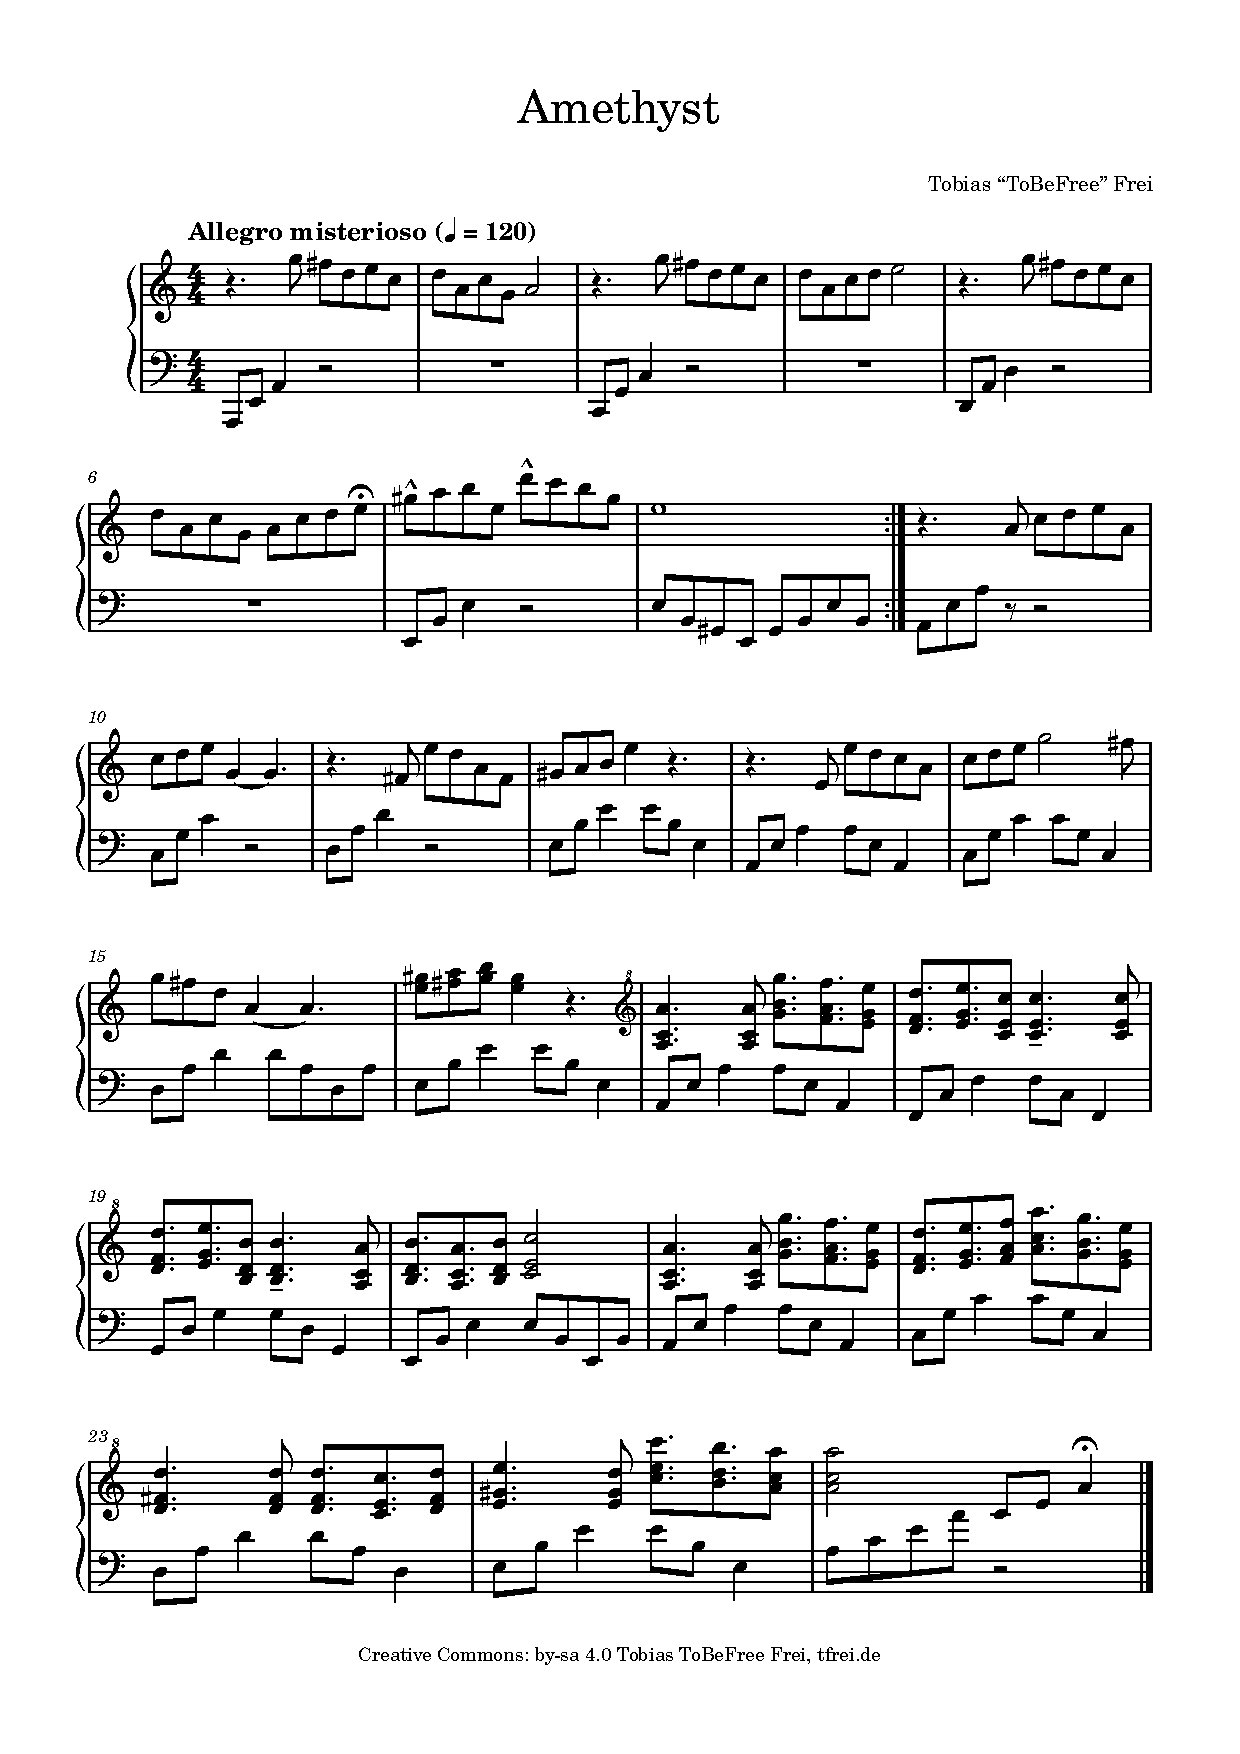
\includegraphics[width=\textwidth, page=1]{z-include-amethyst.pdf}
\end{figure}


\chapter{Musikliste}

\textbf{Für Filmproduzenten, Träumer und Multitasking-Genies.}

\begin{itemize}
    \item Falls Du ernsthaft einen Film zu diesem Buch drehen möchtest.
    \item Falls Du das gesamte Buch bereits ausgelesen hast und die genannten Lieder vielleicht noch nicht kennst. Höre die Lieder und stelle Dir dabei die Szenen vor. Wenn es schon keinen Fnbsrd-Film gibt, kannst Du wenigstens einen Film in deinem Kopf laufen lassen.
    \item Falls Du beim Lesen Musik hören möchtest, die zur aktuellen Szene passt.
\end{itemize}

Diese Liste wurde von Tobias Frei zusammengestellt und impliziert keinerlei Unterstützung oder Befürwortung durch die Komponisten der Lieder. Eines Tages wird jedes dieser Lieder in die Gemeinfreiheit übergehen; der genaue Zeitpunkt hängt von verschiedenen Gesetzen ab.

\begin{enumerate}
    \item Titelmelodie:\\ »Amethyst«~– Tobias »ToBeFree« Frei
    \item \textbf{Teil 1: Exodus.}\\ »Träumen«~– Solitary Experiments featuring In Strict Confidence
    \item Unwillkommenheit:\\ »Spectres from the Black Moss«~– Ashbury Heights
    \item Auf Nimmerwiedersehen:\\ »Oh Johnny«~– Jan Delay
    \item Vor den Mauern der letzten Hoffnung:\\ »Storm«~– Assemblage 23
    \item Willkommen in Last Hope:\\ »Lieder der Freiheit«~– Santiano
    \item Wirtschaftslektion am Tisch:\\ »Crash and Burn«~– Solitary Experiments
    \item Fnbsrd vor der Tür:\\ »Diese kalte Nacht«~– Faun
    \item Am schwarzen Brett:\\ »To Hell and Back«~– Sabaton (Acoustic Cover by Beyond the Black)
    \item Erste Nacht in Last Hope:\\ »The One Eyed King«~– Jacco Gardner
    \item Erwachen im Morgengrauen:\\ »Ride«~– Refuzion featuring LXCPR
    \item Rührei:\\ »Diaries«~– The Birthday Massacre
    \item Dunkelschlag:\\ »Half God Half Devil«~– In This Moment
    \item Unter Flügeln:\\ »Chrono«~– Kraftwerk
    \item Bibliotheksverschwörung:\\ »Teufelsgeiger«~– dArtagnan
    \item Türtechnik:\\ »Revengeance Machine«~– Beast in Black
    \item Licht und Weltsteine:\\ »Days Before You Died«~– Volturian
    \item Schwarze Magie:\\ »Fading Light«~– Aviators
    \item Fnbsrd taucht ab:\\ »The Start of Something New«~– Chrom
    \item Das Innere des Weltsteins:\\ »Red Stars«~– The Birthday Massacre
    \item Das Wesen der Schwerkraft:\\ »Oceandeep«~– Beast in Black
    \item Aufstieg:\\ »Right Here, Right Now«~– Fatboy Slim
    \item Aqua erscheint:\\ »Nincs üzenet«~– Kiss-Gidófalvy-Band
    \item Kornsuche für blinde Hühner:\\ »Superstition«~– The Birthday Massacre
    \item Zeigefinger im Stern:\\ »I Miss the Misery«~– Halestorm
    \item Das Lichtportal:\\ »The One Eyed King«~– Jacco Gardner
    \item Weltkreation:\\ »Magic Pie«~– Oasis
    \item Wesensdiskussion:\\ »Clear the Air«~– Jacco Gardner
    \item Nachtspaziergang:\\ »Chameleon«~– Jacco Gardner
    \item \textbf{Teil 2: Leviticus.}\\ »Free Me«~– Beyond the Black
    \item Zeitwechsel:\\ »Smaller«~– Ashbury Heights
    \item Lindenbibliothek, die Zweite:\\ »Hotel California«~– Eagles
    \item Abschiedskuss in der Bibliothek:\\ »In The Dark«~– Sonata Arctica
    \item Ostkneipe, die Zweite:\\ »Winter is Coming«~– Beyond the Black
    \item Fnbsrd verlässt Last Hope:\\ »Lose Yourself«~– Eminem
    \item Buntes Laub:\\ »All as One«~– Miracle of Sound
    \item Angreifer im Nebel:\\ »Infinite«~– Assemblage 23
    \item Vor den Toren von Alpha:\\ »To The Grave«~– Aviators
    \item Zur goldenen Kanone:\\ »Into the Black«~– Aviators
    \item Ellen erscheint:\\ »Shallow Grave«~– The Birthday Massacre
    \item Kneipendiskussion:\\ »Skin«~– Assemblage 23
    \item Auszug aus Alpha:\\ »Two Hearts«~– The Birthday Massacre
    \item Ferne im Mittagslicht:\\ »You Walk Away«~– Blutengel
    \item Magischer Austausch:\\ »Space and Time«~– She Hates Emotions
    \item Pfeil im Baum:\\ »Train«~– Younger Brother
    \item Cygnistag:\\ »Force of Nature«~– Miracle of Sound und Sarah Murray
    \item Am Mutterbaum:\\ »Lied der Zeit«~– Oonagh
    \item Zwergengesang, Teil 1:\\ »Dark History«~– Blutengel
    \item Zwergengesang, Teil 2:\\ »Irish Way«~– The O’Reillys and the Paddyhats
    \item Strategieverlust:\\ »Tourner Dans Le Vide«~– Indila
    \item Vängäs Auftritt:\\ »Phantasmagoria«~– Ashbury Heights
    \item Vängäs Hütte:\\ »Dream On«~– Aerosmith
    \item Cygnisnacht:\\ »The Sweet Escape«~– Poets of the Fall
    \item Deckenlicht:\\ »The Poet and the Muse«\\~– Old Gods of Asgard (Poets of the Fall)
    \item Morgengrauen unter Tannen:\\ »Oceandeep«~– Poets of the Fall
    \item Aufbruch:\\ »Wake the White Wolf«~– Miracle of Sound
    \item Reise durch die Nacht:\\ »Dark Water«~– Amy Lee und Malika Zarra
    \item Überfall:\\ »Blue«~– The Birthday Massacre
    \item (in Zeitlupe) Ellens Reaktion:\\ »So Young«~– Portugal. The Man
    \item Silberschwert:\\ »Riverside«~– Sidney Samson
    \item Erwachen bei Fisch:\\ »Fresenhof«~– Knut Kiesewetter
    \item Fortsetzung der Reise:\\ »Phantasmagoria«~– Ashbury Heights
    \item Rubine im Mittagslicht:\\ »The Ghost Inside«~– Broken Bells
    \item Letztes Wegstück zum Ozean:\\ »Chanson de Roland«~– dArtagnan
    \item Pavonis am Horizont:\\ »When the Rain Begins to Fall«~– Jermaine Jackson und Pia Zadora
    \item Zur Bastille:\\ »Freedom«~– Richie Havens
    \item Von der Bastille:\\ »Number One«~– Portugal. The Man
    \item Durch das Stadttor:\\ »No Dream Can Heal a Broken Heart«~– Sonata Arctica
    \item Hologrammscheine:\\ »Money, Money, Money«~– ABBA
    \item Rote Doppelaxt:\\ »Touch in the Night«~– Battle Beast
    \item Moralphilosophie:\\ »The Quest and the Curse«~– Delain
    \item Abenddämmerung:\\ »Skyfall«~– Adele
    \item Die Holzbank:\\ »Wide Awake«~– Beyond the Black
    \item Laternenpfad:\\ »Hell to the Heavens«~– Leaves’ Eyes
    \item Abendmahl:\\ »Storytime«~– Nightwish
    \item Erste Nacht in Pavonis:\\ »West Coast«~– Lana Del Rey
    \item Bank im Mondlicht:\\ »Lost on You«~– LP
    \item Gedanken an Cygnis:\\ »My Land«~– Sonata Arctica
    \item Der Drache als Anschauungsobjekt:\\ »Zeroes«~– Sonata Arctica
    \item Parkbank am See:\\ »We Stand Alone«~– Covenant
    \item Zweite Nacht in Pavonis:\\ »Bullet«~– Covenant
    \item Pfefferfrühstück:\\ »Don’t Say A Word«~– Sonata Arctica
    \item Metalldämmerung:\\ »The Final Lullaby«~– Epica und Shining (Norwegen)
    \item Vereitelung:\\ »Mermaids«~– Ignea und Ersedu
    \item Stadtwache:\\ »Jinnslammer«~– Ignea
    \item Finale:\\ »Beneath A Blackened Sky«~– Beyond the Black
    \item Luftlosigkeit:\\ »Breathe«~– Prodigy
    \item Rubinfeuer:\\ »Invictus«~– Delain
    \item Wiedersehen mit Kuss:\\ »Runaway«~– Ladytron
    \item Käfigbruch:\\ »Let it Roar«~– Battle Beast
    \item Amethyst in der Dunkelheit:\\ »Black«~– Blutengel
    \item Heimweg:\\ »Signs of Life«~– Poets of the Fall
    \item Abschied von Vängä:\\ »Tallulah«~– Sonata Arctica
    \item Spurloses Laub:\\ »No Roots«~– Alice Merton
    \item Am Osttor von Last Hope:\\ »Paradise«~– Within Temptation
    \item Silber und Blau:\\ »Gimme! Gimme! Gimme!«~– ABBA
    \item Outro:\\ »Perfect«~– Miracle of Sound und Karliene
    \item Postskriptum:\\ »How I Hate the Night«~– Ignea
\end{enumerate}


\chapter{Bildquellen}

Alle verwendeten Bilder sind gemeinfrei. Die Verwendung der Bilder in diesem Roman impliziert keinerlei Unterstützung oder Befürwortung durch ihre Schöpfer.

\begin{itemize}
    \item \textbf{Buchcover:} CC0-Lizenz / Public Domain.\\ Florian Kurz (flo222, Pixabay vor 2019)
    \item \textbf{Titelbild des zweiten Teils:} CC0-Lizenz / Public Domain.\\ Mabel Amber (MabelAmber, Pixabay vor 2019)
    \item \textbf{Cygniswald:} CC0-Lizenz / Public Domain.\\ Florian Kurz (flo222, Pixabay vor 2019)
\end{itemize}

Bei den Bildern in diesem Roman handelt es sich nicht um die exakten Originalbilder, sondern um Abwandlungen (Weißabgleich, Helligkeit, Kontrast, Sättigung, Schärfung, Zuschnitt etc.) erstellt durch Tobias Frei.


\chapter{Lizenz des Buchinhalts}

\textbf{Fnbsrd © by\\ Tobias Frei, fnbsrd.de}

Dies ist eine offizielle Ausgabe des ersten Fnbsrd-Romans, herausgegeben von Tobias Frei. Veränderte Versionen und unautorisierte Nachdrucke müssen deutlich als solche erkennbar sein. Auch das Impressum muss angepasst werden, wenn das Dokument verändert wird.

Falls du die Rechte in dieser Lizenz nutzen möchtest, musst du sie vollständig gelesen und verstanden haben. Es genügt nicht, nur eine Zusammenfassung zu lesen. Aus diesem Grund wird in diesem Buch keine Zusammenfassung angeboten.

This novel is licensed under a Creative Commons Attribution-ShareAlike 4.0 International License.

You should have received a copy of the license along with this work. If not, see\\
https://creativecommons.org/licenses/by-sa/4.0/legalcode

You are required to actually read and understand the full text of the license, not a summary.

\begin{center}
    \large{\textbf{Creative Commons Attribution-ShareAlike 4.0 International Public License}}
\end{center}

By exercising the Licensed Rights (defined below), You accept and agree to be bound by the terms and conditions of this Creative Commons Attribution-ShareAlike 4.0 International Public License ("Public License"). To the extent this Public License may be interpreted as a contract, You are granted the Licensed Rights in consideration of Your acceptance of these terms and conditions, and the Licensor grants You such rights in consideration of benefits the Licensor receives from making the Licensed Material available under these terms and conditions.

\begin{center}
    \textbf{Section 1 -- Definitions.}
\end{center}

\begin{itemize}
    \item[a.] \textbf{Adapted Material} means material subject to Copyright and Similar Rights that is derived from or based upon the Licensed Material and in which the Licensed Material is translated, altered, arranged, transformed, or otherwise modified in a manner requiring permission under the Copyright and Similar Rights held by the Licensor. For purposes of this Public License, where the Licensed Material is a musical work, performance, or sound recording, Adapted Material is always produced where the Licensed Material is synched in timed relation with a moving image.
    \item[b.] \textbf{Adapter's License} means the license You apply to Your Copyright and Similar Rights in Your contributions to Adapted Material in accordance with the terms and conditions of this Public License.
    \item[c.] \textbf{BY-SA Compatible License} means a license listed at creativecommons.org/compatiblelicenses, approved by Creative Commons as essentially the equivalent of this Public License.
    \item[d.] \textbf{Copyright and Similar Rights} means copyright and/or similar rights closely related to copyright including, without limitation, performance, broadcast, sound recording, and Sui Generis Database Rights, without regard to how the rights are labeled or categorized. For purposes of this Public License, the rights specified in Section 2(b)(1)-(2) are not Copyright and Similar Rights.
    \item[e.] \textbf{Effective Technological Measures} means those measures that, in the absence of proper authority, may not be circumvented under laws fulfilling obligations under Article 11 of the WIPO Copyright Treaty adopted on December 20, 1996, and/or similar international agreements.
    \item[f.] \textbf{Exceptions and Limitations} means fair use, fair dealing, and/or any other exception or limitation to Copyright and Similar Rights that applies to Your use of the Licensed Material.
    \item[g.] \textbf{License Elements} means the license attributes listed in the name of a Creative Commons Public License. The License Elements of this Public License are Attribution and ShareAlike.
    \item[h.] \textbf{Licensed Material} means the artistic or literary work, database, or other material to which the Licensor applied this Public License.
    \item[i.] \textbf{Licensed Rights} means the rights granted to You subject to the terms and conditions of this Public License, which are limited to all Copyright and Similar Rights that apply to Your use of the Licensed Material and that the Licensor has authority to license.
    \item[j.] \textbf{Licensor} means the individual(s) or entity(ies) granting rights under this Public License.
    \item[k.] \textbf{Share} means to provide material to the public by any means or process that requires permission under the Licensed Rights, such as reproduction, public display, public performance, distribution, dissemination, communication, or importation, and to make material available to the public including in ways that members of the public may access the material from a place and at a time individually chosen by them.
    \item[l.] \textbf{Sui Generis Database Rights} means rights other than copyright resulting from Directive 96/9/EC of the European Parliament and of the Council of 11 March 1996 on the legal protection of databases, as amended and/or succeeded, as well as other essentially equivalent rights anywhere in the world.
    \item[m.] \textbf{You} means the individual or entity exercising the Licensed Rights under this Public License. Your has a corresponding meaning.
\end{itemize}

\begin{center}
    \textbf{Section 2 -- Scope.}
\end{center}

\begin{itemize}
    \item[a.] \textbf{License grant.}
    \begin{itemize}
        \item[1.] Subject to the terms and conditions of this Public License, the Licensor hereby grants You a worldwide, royalty-free, non-sublicensable, non-exclusive, irrevocable license to exercise the Licensed Rights in the Licensed Material to:
        \begin{itemize}
            \item[A.] reproduce and Share the Licensed Material, in whole or in part; and
            \item[B.] produce, reproduce, and Share Adapted Material.
        \end{itemize}
        \item[2.] \underline{Exceptions and Limitations}. For the avoidance of doubt, where Exceptions and Limitations apply to Your use, this Public License does not apply, and You do not need to comply with its terms and conditions.
        \item[3.] \underline{Term}. The term of this Public License is specified in Section 6(a).
        \item[4.] \underline{Media and formats; technical modifications allowed}. The Licensor authorizes You to exercise the Licensed Rights in all media and formats whether now known or hereafter created, and to make technical modifications necessary to do so. The Licensor waives and/or agrees not to assert any right or authority to forbid You from making technical modifications necessary to exercise the Licensed Rights, including technical modifications necessary to circumvent Effective Technological Measures. For purposes of this Public License, simply making modifications authorized by this Section 2(a)(4) never produces Adapted Material.
        \item[5.] \underline{Downstream recipients}.
        \begin{itshape}\begin{itemize}
            \item[A.] \underline{Offer from the Licensor -- Licensed Material}. Every recipient of the Licensed Material automatically receives an offer from the Licensor to exercise the Licensed Rights under the terms and conditions of this Public License.
            \item[B.] \underline{Additional offer from the Licensor -- Adapted Material}. Every recipient of Adapted Material from You automatically receives an offer from the Licensor to exercise the Licensed Rights in the Adapted Material under the conditions of the Adapter's License You apply.
            \item[C.] \underline{No downstream restrictions}. You may not offer or impose any additional or different terms or conditions on, or apply any Effective Technological Measures to, the Licensed Material if doing so restricts exercise of the Licensed Rights by any recipient of the Licensed Material.
        \end{itemize}\end{itshape}
        \item[6.] \underline{No endorsement}. Nothing in this Public License constitutes or may be construed as permission to assert or imply that You are, or that Your use of the Licensed Material is, connected with, or sponsored, endorsed, or granted official status by, the Licensor or others designated to receive attribution as provided in Section 3(a)(1)(A)(i).
    \end{itemize}
    \item[b.] \textbf{Other rights.}
    \begin{itemize}
        \item[1.] Moral rights, such as the right of integrity, are not licensed under this Public License, nor are publicity,
          privacy, and/or other similar personality rights; however, to the extent possible, the Licensor waives and/or agrees not to assert any such rights held by the Licensor to the limited extent necessary to allow You to exercise the Licensed Rights, but not otherwise.
        \item[2.] Patent and trademark rights are not licensed under this Public License.
        \item[3.] To the extent possible, the Licensor waives any right to collect royalties from You for the exercise of the Licensed Rights, whether directly or through a collecting society under any voluntary or waivable statutory or compulsory licensing scheme. In all other cases the Licensor expressly reserves any right to collect such royalties.
    \end{itemize}
\end{itemize}

\begin{center}
    \textbf{Section 3 -- License Conditions.}
\end{center}

Your exercise of the Licensed Rights is expressly made subject to the following conditions.

\begin{itemize}
    \item[a.] \textbf{Attribution.}
    \begin{itemize}
        \item[1.] If You Share the Licensed Material (including in modified form), You must:
        \begin{itemize}
            \item[A.] retain the following if it is supplied by the Licensor with the Licensed Material:
            \begin{itemize}
                \item[i.] identification of the creator(s) of the Licensed Material and any others designated to receive attribution, in any reasonable manner requested by the Licensor (including by pseudonym if designated);
                \item[ii.] a copyright notice;
                \item[iii.] a notice that refers to this Public License;
                \item[iv.] a notice that refers to the disclaimer of warranties;
                \item[v.] a URI or hyperlink to the Licensed Material to the extent reasonably practicable;
            \end{itemize}
            \item[B.] indicate if You modified the Licensed Material and retain an indication of any previous modifications; and
            \item[C.] indicate the Licensed Material is licensed under this Public License, and include the text of, or the URI or hyperlink to, this Public License.
        \end{itemize}
        \item[2.] You may satisfy the conditions in Section 3(a)(1) in any reasonable manner based on the medium, means, and context in which You Share the Licensed Material. For example, it may be reasonable to satisfy the conditions by providing a URI or hyperlink to a resource that includes the required information.
        \item[3.] If requested by the Licensor, You must remove any of the information required by Section 3(a)(1)(A) to the extent reasonably practicable.
    \end{itemize}
    \item[b.] \textbf{ShareAlike.}

     In addition to the conditions in Section 3(a), if You Share Adapted Material You produce, the following conditions also apply.

    \begin{itemize}
        \item[1.] The Adapter's License You apply must be a Creative Commons license with the same License Elements, this version or later, or a BY-SA Compatible License.
        \item[2.] You must include the text of, or the URI or hyperlink to, the Adapter's License You apply. You may satisfy this condition in any reasonable manner based on the medium, means, and context in which You Share Adapted Material.
        \item[3.] You may not offer or impose any additional or different terms or conditions on, or apply any Effective Technological Measures to, Adapted Material that restrict exercise of the rights granted under the Adapter's License You apply.
    \end{itemize}
\end{itemize}

\begin{center}
    \textbf{Section 4 -- Sui Generis Database Rights.}
\end{center}

Where the Licensed Rights include Sui Generis Database Rights that apply to Your use of the Licensed Material:

\begin{itemize}
    \item[a.] for the avoidance of doubt, Section 2(a)(1) grants You the right to extract, reuse, reproduce, and Share all or a substantial portion of the contents of the database;
    \item[b.] if You include all or a substantial portion of the database contents in a database in which You have Sui Generis Database Rights, then the database in which You have Sui Generis Database Rights (but not its individual contents) is Adapted Material, including for purposes of Section 3(b); and
    \item[c.] You must comply with the conditions in Section 3(a) if You Share all or a substantial portion of the contents of the database.
\end{itemize}

For the avoidance of doubt, this Section 4 supplements and does not replace Your obligations under this Public License where the Licensed Rights include other Copyright and Similar Rights.

\begin{center}
    \textbf{Section 5 -- Disclaimer of Warranties and Limitation of Liability.}
\end{center}

\begin{itemize}
    \item[\textbf{a.}] \textbf{Unless otherwise separately undertaken by the Licensor, to the extent possible, the Licensor offers the Licensed Material as-is and as-available, and makes no representations or warranties of any kind concerning the Licensed Material, whether express, implied, statutory, or other. This includes, without limitation, warranties of title, merchantability, fitness for a particular purpose, non-infringement, absence of latent or other defects, accuracy, or the presence or absence of errors, whether or not known or discoverable. Where disclaimers of warranties are not allowed in full or in part, this disclaimer may not apply to You.}
    \item[\textbf{b.}] \textbf{To the extent possible, in no event will the Licensor be liable to You on any legal theory (including, without limitation, negligence) or otherwise for any direct, special, indirect, incidental, consequential, punitive, exemplary, or other losses, costs, expenses, or damages arising out of this Public License or use of the Licensed Material, even if the Licensor has been advised of the possibility of such losses, costs, expenses, or damages. Where a limitation of liability is not allowed in full or in part, this limitation may not apply to You.}
    \item[c.] The disclaimer of warranties and limitation of liability provided above shall be interpreted in a manner that, to the extent possible, most closely approximates an absolute disclaimer and waiver of all liability.
\end{itemize}

\begin{center}
    \textbf{Section 6 -- Term and Termination.}
\end{center}

\begin{itemize}
    \item[a.] This Public License applies for the term of the Copyright and Similar Rights licensed here. However, if You fail to comply with this Public License, then Your rights under this Public License terminate automatically.
    \item[b.] Where Your right to use the Licensed Material has terminated under Section 6(a), it reinstates:
    \begin{itemize}
        \item[1.] automatically as of the date the violation is cured, provided it is cured within 30 days of Your discovery of the violation; or
        \item[2.] upon express reinstatement by the Licensor.
    \end{itemize}

     For the avoidance of doubt, this Section 6(b) does not affect any right the Licensor may have to seek remedies for Your violations of this Public License.

    \item[c.] For the avoidance of doubt, the Licensor may also offer the Licensed Material under separate terms or conditions or stop distributing the Licensed Material at any time; however, doing so will not terminate this Public License.
    \item[d.] Sections 1, 5, 6, 7, and 8 survive termination of this Public License.
\end{itemize}

\begin{center}
    \textbf{Section 7 -- Other Terms and Conditions.}
\end{center}

\begin{itemize}
    \item[a.] The Licensor shall not be bound by any additional or different terms or conditions communicated by You unless expressly agreed.
    \item[b.] Any arrangements, understandings, or agreements regarding the Licensed Material not stated herein are separate from and independent of the terms and conditions of this Public License.
\end{itemize}

\begin{center}
    \textbf{Section 8 -- Interpretation.}
\end{center}

\begin{itemize}
    \item[a.] For the avoidance of doubt, this Public License does not, and shall not be interpreted to, reduce, limit, restrict, or impose conditions on any use of the Licensed Material that could lawfully be made without permission under this Public License.
    \item[b.] To the extent possible, if any provision of this Public License is deemed unenforceable, it shall be automatically reformed to the minimum extent necessary to make it enforceable. If the provision cannot be reformed, it shall be severed from this Public License without affecting the enforceability of the remaining terms and conditions.
    \item[c.] No term or condition of this Public License will be waived and no failure to comply consented to unless expressly agreed to by the Licensor.
    \item[d.] Nothing in this Public License constitutes or may be interpreted as a limitation upon, or waiver of, any privileges and immunities that apply to the Licensor or You, including from the legal processes of any jurisdiction or authority.
\end{itemize}

\end{document}
